%% ============================================================
%% 专题讲座 S2：二元选择模型——非参数方法
%% Special Topics S2: Binary Choice Models — Nonparametric Methods
%% 中级计量经济学（研究生）— 山东财经大学
%% 主要参考：Caetano Nonparametric Lecture Notes Class 1-4;
%%           Li & Racine (2007) Nonparametric Econometrics Ch.2-6;
%%           Zhou Xianbo 《非参数计量经济学》Ch.1-3;
%%           Fan & Gijbels (1996) Local Polynomial Modelling;
%%           Hansen Econometrics Ch.19-20; Horowitz (2009).
%% ============================================================
\documentclass[aspectratio=169, 10pt]{beamer}
% ==============================================================================
% header.tex — LaTeX Preamble for Intermediate Econometrics
% Shandong University of Finance and Economics (SUFE)
% Textbook: Wooldridge, Introductory Econometrics, 8th edition
% ==============================================================================
%
% USAGE (from Slides/ directory):
%   % ==============================================================================
% header.tex — LaTeX Preamble for Intermediate Econometrics
% Shandong University of Finance and Economics (SUFE)
% Textbook: Wooldridge, Introductory Econometrics, 8th edition
% ==============================================================================
%
% USAGE (from Slides/ directory):
%   % ==============================================================================
% header.tex — LaTeX Preamble for Intermediate Econometrics
% Shandong University of Finance and Economics (SUFE)
% Textbook: Wooldridge, Introductory Econometrics, 8th edition
% ==============================================================================
%
% USAGE (from Slides/ directory):
%   \input{header}          % in Beamer .tex files (TEXINPUTS=../Preambles:)
%
% COMPILE (3-pass XeLaTeX):
%   cd Slides
%   TEXINPUTS=../Preambles:$TEXINPUTS xelatex -interaction=nonstopmode file.tex
%   BIBINPUTS=..:$BIBINPUTS bibtex file
%   TEXINPUTS=../Preambles:$TEXINPUTS xelatex -interaction=nonstopmode file.tex
%   TEXINPUTS=../Preambles:$TEXINPUTS xelatex -interaction=nonstopmode file.tex
% ==============================================================================


% --- Essential packages -------------------------------------------------------
\usepackage{fontspec}           % XeLaTeX font support (must load early)
\usepackage{amsmath}            % Math environments (align, equation, etc.)
\usepackage{amssymb}            % Math symbols (mathbb, etc.)
\usepackage{bm}                 % Bold math (\bm{})
\usepackage{mathtools}          % Extended math tools (coloneqq, etc.)


% --- Table packages -----------------------------------------------------------
\usepackage{booktabs}           % Professional tables (\toprule, \midrule, \bottomrule)
\usepackage{threeparttable}     % Table notes (tablenotes environment)
\usepackage{siunitx}            % Number alignment in tables (S column type)
\sisetup{
  table-format = 1.4,
  table-number-alignment = center,
  detect-weight = true,
  detect-inline-weight = math
}


% --- Figure and graphics packages --------------------------------------------
\usepackage{graphicx}           % Include figures (\includegraphics)
\usepackage{subcaption}         % Subfigures (subfigure environment)
\usepackage{tikz}               % TikZ diagrams
\usepackage{pgfplots}           % Data plots
\pgfplotsset{compat=1.18}
\usetikzlibrary{arrows.meta, positioning, shapes.geometric,
                decorations.pathreplacing, calc, patterns}


% --- Color and boxes ----------------------------------------------------------
\usepackage{xcolor}             % Extended color support
\usepackage{tcolorbox}          % Custom box environments
\tcbuselibrary{skins, breakable, theorems}


% --- Other utility packages ---------------------------------------------------
\usepackage{hyperref}           % Hyperlinks
\usepackage{natbib}             % Bibliography (\citet, \citep, \citealt)
\usepackage{caption}            % Figure/table captions
\usepackage{appendixnumberbeamer} % Appendix frame numbering


% ==============================================================================
% SUFE INSTITUTIONAL COLORS
% ==============================================================================
% Update hex values to match official SUFE brand colors if available.

\definecolor{SUFEBlue}{HTML}{012169}     % Primary: deep navy
\definecolor{SUFEGold}{HTML}{B9975B}     % Secondary: warm gold
\definecolor{SUFEYellow}{HTML}{F2A900}   % Highlight: bright gold/yellow
\definecolor{SUFELight}{HTML}{E8EDF5}    % Light background: pale blue-gray
\definecolor{SUFEDark}{HTML}{1a1a1a}     % Body text: near-black
\definecolor{positive}{HTML}{2E7D32}     % Positive/correct: dark green
\definecolor{negative}{HTML}{C62828}     % Negative/incorrect: dark red


% ==============================================================================
% BEAMER THEME & COLOR SETUP
% ==============================================================================

\usetheme{default}
\useinnertheme{default}
\useoutertheme{default}
\usecolortheme{default}

% Frame title
\setbeamercolor{frametitle}{fg=SUFEBlue, bg=white}
\setbeamerfont{frametitle}{size=\large, series=\bfseries}
\setbeamertemplate{frametitle}[default][left]
\addtobeamertemplate{frametitle}{\vspace{0.05em}}{%
  \vspace{0.05em}{\color{SUFEGold}\rule{\textwidth}{0.5pt}}\vspace{-0.1em}}

% Title page
\setbeamercolor{title}{fg=SUFEBlue}
\setbeamercolor{subtitle}{fg=SUFEGold}
\setbeamercolor{author}{fg=SUFEBlue}
\setbeamercolor{institute}{fg=SUFEDark}
\setbeamercolor{date}{fg=SUFEGold}

% Structure elements
\setbeamercolor{structure}{fg=SUFEBlue}
\setbeamercolor{item}{fg=SUFEBlue}
\setbeamercolor{subitem}{fg=SUFEGold}
\setbeamercolor{subsubitem}{fg=SUFEGold}
\setbeamerfont{itemize/enumerate body}{size=\normalsize}
\setbeamerfont{itemize/enumerate subbody}{size=\small}

% Block environments
\setbeamercolor{block title}{fg=white, bg=SUFEBlue}
\setbeamercolor{block body}{fg=SUFEDark, bg=SUFELight}
\setbeamercolor{block title alerted}{fg=white, bg=red!70!black}
\setbeamercolor{block body alerted}{fg=SUFEDark, bg=red!5}
\setbeamercolor{block title example}{fg=white, bg=SUFEGold!80!black}
\setbeamercolor{block body example}{fg=SUFEDark, bg=SUFEGold!8}

% Remove navigation symbols
\setbeamertemplate{navigation symbols}{}

% Footline: author | short title | slide N/N
\setbeamertemplate{footline}{%
  \leavevmode%
  \hbox{%
    \begin{beamercolorbox}[wd=.30\paperwidth,ht=2.25ex,dp=1ex,left,leftskip=2mm]{author in head/foot}%
      \usebeamerfont{author in head/foot}\insertshortauthor
    \end{beamercolorbox}%
    \begin{beamercolorbox}[wd=.40\paperwidth,ht=2.25ex,dp=1ex,center]{title in head/foot}%
      \usebeamerfont{title in head/foot}\insertshorttitle
    \end{beamercolorbox}%
    \begin{beamercolorbox}[wd=.30\paperwidth,ht=2.25ex,dp=1ex,right,rightskip=2mm]{date in head/foot}%
      \usebeamerfont{date in head/foot}%
      \insertframenumber{} / \inserttotalframenumber
    \end{beamercolorbox}}%
  \vskip0pt%
}
\setbeamercolor{author in head/foot}{fg=white, bg=SUFEBlue}
\setbeamercolor{title in head/foot}{fg=white, bg=SUFEBlue!80!black}
\setbeamercolor{date in head/foot}{fg=white, bg=SUFEBlue}

% Section separator slides (large centered section title)
\AtBeginSection[]{
  \begin{frame}
    \centering
    \vfill
    {\Large\bfseries\color{SUFEBlue}\insertsectionhead}
    \vfill
    {\color{SUFEGold}\rule{0.5\textwidth}{1pt}}
    \vfill
  \end{frame}
}


% ==============================================================================
% FONT SETUP (XeLaTeX)
% ==============================================================================
% Using Windows system fonts (Times New Roman / Arial / Consolas).
% On macOS, swap for: TeX Gyre Termes / TeX Gyre Heros / TeX Gyre Cursor
%   or: Times New Roman / Helvetica / Courier New

\setmainfont{Times New Roman}
\setsansfont{Arial}
\setmonofont{Consolas}


% ==============================================================================
% CUSTOM BOX ENVIRONMENTS (tcolorbox)
% ==============================================================================
% Quarto CSS equivalents: .keybox, .highlightbox, .methodbox,
%                         .assumptionbox, .resultbox

% keybox: key definitions, stated assumptions
\newtcolorbox{keybox}{
  enhanced,
  colback  = SUFEGold!10!white,
  colframe = SUFEGold,
  leftrule = 4pt, rightrule = 0pt, toprule = 0pt, bottomrule = 0pt,
  arc = 0pt, outer arc = 0pt,
  boxsep = 0pt, left = 8pt, right = 6pt, top = 4pt, bottom = 4pt,
}

% highlightbox: important theorems, main results
\newtcolorbox{highlightbox}{
  enhanced,
  colback  = SUFEYellow!8!white,
  colframe = SUFEYellow!80!SUFEGold,
  leftrule = 4pt, rightrule = 0pt, toprule = 0pt, bottomrule = 0pt,
  arc = 0pt, outer arc = 0pt,
  boxsep = 0pt, left = 8pt, right = 6pt, top = 4pt, bottom = 4pt,
}

% definitionbox{Title}: formal definitions — OLS, IV, GMM, etc.
\newtcolorbox{definitionbox}[1]{
  enhanced,
  title    = #1,
  colback  = SUFEBlue!4!white,
  colframe = SUFEBlue,
  colbacktitle = SUFEBlue,
  coltitle = white,
  fonttitle= \bfseries\small,
  arc = 4pt, outer arc = 4pt,
  boxsep = 0pt, left = 8pt, right = 6pt, top = 4pt, bottom = 4pt,
  toptitle = 3pt, bottomtitle = 3pt,
}

% examplebox{Title}: empirical examples, Wooldridge data applications
\newtcolorbox{examplebox}[1]{
  enhanced,
  title    = #1,
  colback  = SUFELight,
  colframe = SUFEGold!70!white,
  colbacktitle = SUFEGold!35!white,
  coltitle = SUFEBlue,
  fonttitle= \bfseries\small,
  arc = 4pt, outer arc = 4pt,
  boxsep = 0pt, left = 8pt, right = 6pt, top = 4pt, bottom = 4pt,
  toptitle = 3pt, bottomtitle = 3pt,
}

% assumptionbox: numbered OLS assumptions (MLR.1–MLR.6)
\newtcolorbox{assumptionbox}{
  enhanced,
  colback  = SUFEGold!8!white,
  colframe = SUFEGold,
  arc = 4pt, outer arc = 4pt,
  boxsep = 0pt, left = 8pt, right = 6pt, top = 4pt, bottom = 4pt,
}


% ==============================================================================
% STANDARD MATH MACROS
% ==============================================================================

% --- Operators ----------------------------------------------------------------
\DeclareMathOperator{\E}{\mathbb{E}}       % Expectation
\DeclareMathOperator{\Var}{Var}             % Variance
\DeclareMathOperator{\Cov}{Cov}             % Covariance
\DeclareMathOperator{\Corr}{Corr}           % Correlation
\DeclareMathOperator{\plim}{plim}           % Probability limit
\DeclareMathOperator{\rank}{rank}           % Matrix rank
\DeclareMathOperator{\tr}{tr}               % Matrix trace
\DeclareMathOperator{\se}{se}               % Standard error

% --- Common shortcuts ---------------------------------------------------------
\newcommand{\bhat}{\hat{\beta}}             % OLS point estimator
\newcommand{\bhatt}{\tilde{\beta}}          % Alternative estimator
\newcommand{\eps}{\varepsilon}              % Error term
\newcommand{\epsh}{\hat{\varepsilon}}       % OLS residual
\newcommand{\uh}{\hat{u}}                   % Residual (alternative)
\newcommand{\yh}{\hat{y}}                   % Fitted value

% Matrices and vectors
\newcommand{\Xb}{\mathbf{X}}               % Design matrix
\newcommand{\yb}{\mathbf{y}}               % Outcome vector
\newcommand{\betab}{\boldsymbol{\beta}}    % Parameter vector
\newcommand{\epsb}{\boldsymbol{\varepsilon}} % Error vector

% Goodness-of-fit
\newcommand{\SSR}{\text{SSR}}              % Sum of squared residuals
\newcommand{\SSE}{\text{SSE}}              % Explained sum of squares
\newcommand{\SST}{\text{SST}}              % Total sum of squares
\newcommand{\Rsq}{R^2}                     % R-squared
\newcommand{\aRsq}{\bar{R}^2}             % Adjusted R-squared

% Asymptotic notation
\newcommand{\avar}{\text{Avar}}            % Asymptotic variance
\newcommand{\pto}{\overset{p}{\to}}        % Convergence in probability
\newcommand{\dto}{\overset{d}{\to}}        % Convergence in distribution
\newcommand{\iid}{\overset{\text{iid}}{\sim}}  % i.i.d. distributed
\newcommand{\asim}{\overset{a}{\sim}}      % Approximately distributed

% Econometric estimators
\newcommand{\OLS}{\text{OLS}}
\newcommand{\IV}{\text{IV}}
\newcommand{\TSLS}{\text{2SLS}}
\newcommand{\GMM}{\text{GMM}}
\newcommand{\FE}{\text{FE}}
\newcommand{\RE}{\text{RE}}
\newcommand{\DID}{\text{DiD}}
\newcommand{\RD}{\text{RD}}

% Probability
\newcommand{\prob}{\mathbb{P}}             % Probability
\newcommand{\indep}{\perp\!\!\!\perp}      % Statistical independence

% Distributions
\newcommand{\Normal}{\mathcal{N}}          % Normal distribution
% Usage: X \sim \Normal(\mu, \sigma^2)

% Absolute value and norm
\newcommand{\abs}[1]{\left\lvert #1 \right\rvert}
\newcommand{\norm}[1]{\left\lVert #1 \right\rVert}


% ==============================================================================
% HYPERREF SETUP
% ==============================================================================

\hypersetup{
  colorlinks = true,
  linkcolor  = SUFEBlue,
  citecolor  = SUFEGold,
  urlcolor   = SUFEBlue
}


% ==============================================================================
% BIBLIOGRAPHY SETUP
% ==============================================================================

\bibliographystyle{aer}   % American Economic Review style
% Usage: \bibliography{../Bibliography_base}  (from Slides/ directory)
% In-text: \citet{Wooldridge2020}, \citep{White1980}
          % in Beamer .tex files (TEXINPUTS=../Preambles:)
%
% COMPILE (3-pass XeLaTeX):
%   cd Slides
%   TEXINPUTS=../Preambles:$TEXINPUTS xelatex -interaction=nonstopmode file.tex
%   BIBINPUTS=..:$BIBINPUTS bibtex file
%   TEXINPUTS=../Preambles:$TEXINPUTS xelatex -interaction=nonstopmode file.tex
%   TEXINPUTS=../Preambles:$TEXINPUTS xelatex -interaction=nonstopmode file.tex
% ==============================================================================


% --- Essential packages -------------------------------------------------------
\usepackage{fontspec}           % XeLaTeX font support (must load early)
\usepackage{amsmath}            % Math environments (align, equation, etc.)
\usepackage{amssymb}            % Math symbols (mathbb, etc.)
\usepackage{bm}                 % Bold math (\bm{})
\usepackage{mathtools}          % Extended math tools (coloneqq, etc.)


% --- Table packages -----------------------------------------------------------
\usepackage{booktabs}           % Professional tables (\toprule, \midrule, \bottomrule)
\usepackage{threeparttable}     % Table notes (tablenotes environment)
\usepackage{siunitx}            % Number alignment in tables (S column type)
\sisetup{
  table-format = 1.4,
  table-number-alignment = center,
  detect-weight = true,
  detect-inline-weight = math
}


% --- Figure and graphics packages --------------------------------------------
\usepackage{graphicx}           % Include figures (\includegraphics)
\usepackage{subcaption}         % Subfigures (subfigure environment)
\usepackage{tikz}               % TikZ diagrams
\usepackage{pgfplots}           % Data plots
\pgfplotsset{compat=1.18}
\usetikzlibrary{arrows.meta, positioning, shapes.geometric,
                decorations.pathreplacing, calc, patterns}


% --- Color and boxes ----------------------------------------------------------
\usepackage{xcolor}             % Extended color support
\usepackage{tcolorbox}          % Custom box environments
\tcbuselibrary{skins, breakable, theorems}


% --- Other utility packages ---------------------------------------------------
\usepackage{hyperref}           % Hyperlinks
\usepackage{natbib}             % Bibliography (\citet, \citep, \citealt)
\usepackage{caption}            % Figure/table captions
\usepackage{appendixnumberbeamer} % Appendix frame numbering


% ==============================================================================
% SUFE INSTITUTIONAL COLORS
% ==============================================================================
% Update hex values to match official SUFE brand colors if available.

\definecolor{SUFEBlue}{HTML}{012169}     % Primary: deep navy
\definecolor{SUFEGold}{HTML}{B9975B}     % Secondary: warm gold
\definecolor{SUFEYellow}{HTML}{F2A900}   % Highlight: bright gold/yellow
\definecolor{SUFELight}{HTML}{E8EDF5}    % Light background: pale blue-gray
\definecolor{SUFEDark}{HTML}{1a1a1a}     % Body text: near-black
\definecolor{positive}{HTML}{2E7D32}     % Positive/correct: dark green
\definecolor{negative}{HTML}{C62828}     % Negative/incorrect: dark red


% ==============================================================================
% BEAMER THEME & COLOR SETUP
% ==============================================================================

\usetheme{default}
\useinnertheme{default}
\useoutertheme{default}
\usecolortheme{default}

% Frame title
\setbeamercolor{frametitle}{fg=SUFEBlue, bg=white}
\setbeamerfont{frametitle}{size=\large, series=\bfseries}
\setbeamertemplate{frametitle}[default][left]
\addtobeamertemplate{frametitle}{\vspace{0.05em}}{%
  \vspace{0.05em}{\color{SUFEGold}\rule{\textwidth}{0.5pt}}\vspace{-0.1em}}

% Title page
\setbeamercolor{title}{fg=SUFEBlue}
\setbeamercolor{subtitle}{fg=SUFEGold}
\setbeamercolor{author}{fg=SUFEBlue}
\setbeamercolor{institute}{fg=SUFEDark}
\setbeamercolor{date}{fg=SUFEGold}

% Structure elements
\setbeamercolor{structure}{fg=SUFEBlue}
\setbeamercolor{item}{fg=SUFEBlue}
\setbeamercolor{subitem}{fg=SUFEGold}
\setbeamercolor{subsubitem}{fg=SUFEGold}
\setbeamerfont{itemize/enumerate body}{size=\normalsize}
\setbeamerfont{itemize/enumerate subbody}{size=\small}

% Block environments
\setbeamercolor{block title}{fg=white, bg=SUFEBlue}
\setbeamercolor{block body}{fg=SUFEDark, bg=SUFELight}
\setbeamercolor{block title alerted}{fg=white, bg=red!70!black}
\setbeamercolor{block body alerted}{fg=SUFEDark, bg=red!5}
\setbeamercolor{block title example}{fg=white, bg=SUFEGold!80!black}
\setbeamercolor{block body example}{fg=SUFEDark, bg=SUFEGold!8}

% Remove navigation symbols
\setbeamertemplate{navigation symbols}{}

% Footline: author | short title | slide N/N
\setbeamertemplate{footline}{%
  \leavevmode%
  \hbox{%
    \begin{beamercolorbox}[wd=.30\paperwidth,ht=2.25ex,dp=1ex,left,leftskip=2mm]{author in head/foot}%
      \usebeamerfont{author in head/foot}\insertshortauthor
    \end{beamercolorbox}%
    \begin{beamercolorbox}[wd=.40\paperwidth,ht=2.25ex,dp=1ex,center]{title in head/foot}%
      \usebeamerfont{title in head/foot}\insertshorttitle
    \end{beamercolorbox}%
    \begin{beamercolorbox}[wd=.30\paperwidth,ht=2.25ex,dp=1ex,right,rightskip=2mm]{date in head/foot}%
      \usebeamerfont{date in head/foot}%
      \insertframenumber{} / \inserttotalframenumber
    \end{beamercolorbox}}%
  \vskip0pt%
}
\setbeamercolor{author in head/foot}{fg=white, bg=SUFEBlue}
\setbeamercolor{title in head/foot}{fg=white, bg=SUFEBlue!80!black}
\setbeamercolor{date in head/foot}{fg=white, bg=SUFEBlue}

% Section separator slides (large centered section title)
\AtBeginSection[]{
  \begin{frame}
    \centering
    \vfill
    {\Large\bfseries\color{SUFEBlue}\insertsectionhead}
    \vfill
    {\color{SUFEGold}\rule{0.5\textwidth}{1pt}}
    \vfill
  \end{frame}
}


% ==============================================================================
% FONT SETUP (XeLaTeX)
% ==============================================================================
% Using Windows system fonts (Times New Roman / Arial / Consolas).
% On macOS, swap for: TeX Gyre Termes / TeX Gyre Heros / TeX Gyre Cursor
%   or: Times New Roman / Helvetica / Courier New

\setmainfont{Times New Roman}
\setsansfont{Arial}
\setmonofont{Consolas}


% ==============================================================================
% CUSTOM BOX ENVIRONMENTS (tcolorbox)
% ==============================================================================
% Quarto CSS equivalents: .keybox, .highlightbox, .methodbox,
%                         .assumptionbox, .resultbox

% keybox: key definitions, stated assumptions
\newtcolorbox{keybox}{
  enhanced,
  colback  = SUFEGold!10!white,
  colframe = SUFEGold,
  leftrule = 4pt, rightrule = 0pt, toprule = 0pt, bottomrule = 0pt,
  arc = 0pt, outer arc = 0pt,
  boxsep = 0pt, left = 8pt, right = 6pt, top = 4pt, bottom = 4pt,
}

% highlightbox: important theorems, main results
\newtcolorbox{highlightbox}{
  enhanced,
  colback  = SUFEYellow!8!white,
  colframe = SUFEYellow!80!SUFEGold,
  leftrule = 4pt, rightrule = 0pt, toprule = 0pt, bottomrule = 0pt,
  arc = 0pt, outer arc = 0pt,
  boxsep = 0pt, left = 8pt, right = 6pt, top = 4pt, bottom = 4pt,
}

% definitionbox{Title}: formal definitions — OLS, IV, GMM, etc.
\newtcolorbox{definitionbox}[1]{
  enhanced,
  title    = #1,
  colback  = SUFEBlue!4!white,
  colframe = SUFEBlue,
  colbacktitle = SUFEBlue,
  coltitle = white,
  fonttitle= \bfseries\small,
  arc = 4pt, outer arc = 4pt,
  boxsep = 0pt, left = 8pt, right = 6pt, top = 4pt, bottom = 4pt,
  toptitle = 3pt, bottomtitle = 3pt,
}

% examplebox{Title}: empirical examples, Wooldridge data applications
\newtcolorbox{examplebox}[1]{
  enhanced,
  title    = #1,
  colback  = SUFELight,
  colframe = SUFEGold!70!white,
  colbacktitle = SUFEGold!35!white,
  coltitle = SUFEBlue,
  fonttitle= \bfseries\small,
  arc = 4pt, outer arc = 4pt,
  boxsep = 0pt, left = 8pt, right = 6pt, top = 4pt, bottom = 4pt,
  toptitle = 3pt, bottomtitle = 3pt,
}

% assumptionbox: numbered OLS assumptions (MLR.1–MLR.6)
\newtcolorbox{assumptionbox}{
  enhanced,
  colback  = SUFEGold!8!white,
  colframe = SUFEGold,
  arc = 4pt, outer arc = 4pt,
  boxsep = 0pt, left = 8pt, right = 6pt, top = 4pt, bottom = 4pt,
}


% ==============================================================================
% STANDARD MATH MACROS
% ==============================================================================

% --- Operators ----------------------------------------------------------------
\DeclareMathOperator{\E}{\mathbb{E}}       % Expectation
\DeclareMathOperator{\Var}{Var}             % Variance
\DeclareMathOperator{\Cov}{Cov}             % Covariance
\DeclareMathOperator{\Corr}{Corr}           % Correlation
\DeclareMathOperator{\plim}{plim}           % Probability limit
\DeclareMathOperator{\rank}{rank}           % Matrix rank
\DeclareMathOperator{\tr}{tr}               % Matrix trace
\DeclareMathOperator{\se}{se}               % Standard error

% --- Common shortcuts ---------------------------------------------------------
\newcommand{\bhat}{\hat{\beta}}             % OLS point estimator
\newcommand{\bhatt}{\tilde{\beta}}          % Alternative estimator
\newcommand{\eps}{\varepsilon}              % Error term
\newcommand{\epsh}{\hat{\varepsilon}}       % OLS residual
\newcommand{\uh}{\hat{u}}                   % Residual (alternative)
\newcommand{\yh}{\hat{y}}                   % Fitted value

% Matrices and vectors
\newcommand{\Xb}{\mathbf{X}}               % Design matrix
\newcommand{\yb}{\mathbf{y}}               % Outcome vector
\newcommand{\betab}{\boldsymbol{\beta}}    % Parameter vector
\newcommand{\epsb}{\boldsymbol{\varepsilon}} % Error vector

% Goodness-of-fit
\newcommand{\SSR}{\text{SSR}}              % Sum of squared residuals
\newcommand{\SSE}{\text{SSE}}              % Explained sum of squares
\newcommand{\SST}{\text{SST}}              % Total sum of squares
\newcommand{\Rsq}{R^2}                     % R-squared
\newcommand{\aRsq}{\bar{R}^2}             % Adjusted R-squared

% Asymptotic notation
\newcommand{\avar}{\text{Avar}}            % Asymptotic variance
\newcommand{\pto}{\overset{p}{\to}}        % Convergence in probability
\newcommand{\dto}{\overset{d}{\to}}        % Convergence in distribution
\newcommand{\iid}{\overset{\text{iid}}{\sim}}  % i.i.d. distributed
\newcommand{\asim}{\overset{a}{\sim}}      % Approximately distributed

% Econometric estimators
\newcommand{\OLS}{\text{OLS}}
\newcommand{\IV}{\text{IV}}
\newcommand{\TSLS}{\text{2SLS}}
\newcommand{\GMM}{\text{GMM}}
\newcommand{\FE}{\text{FE}}
\newcommand{\RE}{\text{RE}}
\newcommand{\DID}{\text{DiD}}
\newcommand{\RD}{\text{RD}}

% Probability
\newcommand{\prob}{\mathbb{P}}             % Probability
\newcommand{\indep}{\perp\!\!\!\perp}      % Statistical independence

% Distributions
\newcommand{\Normal}{\mathcal{N}}          % Normal distribution
% Usage: X \sim \Normal(\mu, \sigma^2)

% Absolute value and norm
\newcommand{\abs}[1]{\left\lvert #1 \right\rvert}
\newcommand{\norm}[1]{\left\lVert #1 \right\rVert}


% ==============================================================================
% HYPERREF SETUP
% ==============================================================================

\hypersetup{
  colorlinks = true,
  linkcolor  = SUFEBlue,
  citecolor  = SUFEGold,
  urlcolor   = SUFEBlue
}


% ==============================================================================
% BIBLIOGRAPHY SETUP
% ==============================================================================

\bibliographystyle{aer}   % American Economic Review style
% Usage: \bibliography{../Bibliography_base}  (from Slides/ directory)
% In-text: \citet{Wooldridge2020}, \citep{White1980}
          % in Beamer .tex files (TEXINPUTS=../Preambles:)
%
% COMPILE (3-pass XeLaTeX):
%   cd Slides
%   TEXINPUTS=../Preambles:$TEXINPUTS xelatex -interaction=nonstopmode file.tex
%   BIBINPUTS=..:$BIBINPUTS bibtex file
%   TEXINPUTS=../Preambles:$TEXINPUTS xelatex -interaction=nonstopmode file.tex
%   TEXINPUTS=../Preambles:$TEXINPUTS xelatex -interaction=nonstopmode file.tex
% ==============================================================================


% --- Essential packages -------------------------------------------------------
\usepackage{fontspec}           % XeLaTeX font support (must load early)
\usepackage{amsmath}            % Math environments (align, equation, etc.)
\usepackage{amssymb}            % Math symbols (mathbb, etc.)
\usepackage{bm}                 % Bold math (\bm{})
\usepackage{mathtools}          % Extended math tools (coloneqq, etc.)


% --- Table packages -----------------------------------------------------------
\usepackage{booktabs}           % Professional tables (\toprule, \midrule, \bottomrule)
\usepackage{threeparttable}     % Table notes (tablenotes environment)
\usepackage{siunitx}            % Number alignment in tables (S column type)
\sisetup{
  table-format = 1.4,
  table-number-alignment = center,
  detect-weight = true,
  detect-inline-weight = math
}


% --- Figure and graphics packages --------------------------------------------
\usepackage{graphicx}           % Include figures (\includegraphics)
\usepackage{subcaption}         % Subfigures (subfigure environment)
\usepackage{tikz}               % TikZ diagrams
\usepackage{pgfplots}           % Data plots
\pgfplotsset{compat=1.18}
\usetikzlibrary{arrows.meta, positioning, shapes.geometric,
                decorations.pathreplacing, calc, patterns}


% --- Color and boxes ----------------------------------------------------------
\usepackage{xcolor}             % Extended color support
\usepackage{tcolorbox}          % Custom box environments
\tcbuselibrary{skins, breakable, theorems}


% --- Other utility packages ---------------------------------------------------
\usepackage{hyperref}           % Hyperlinks
\usepackage{natbib}             % Bibliography (\citet, \citep, \citealt)
\usepackage{caption}            % Figure/table captions
\usepackage{appendixnumberbeamer} % Appendix frame numbering


% ==============================================================================
% SUFE INSTITUTIONAL COLORS
% ==============================================================================
% Update hex values to match official SUFE brand colors if available.

\definecolor{SUFEBlue}{HTML}{012169}     % Primary: deep navy
\definecolor{SUFEGold}{HTML}{B9975B}     % Secondary: warm gold
\definecolor{SUFEYellow}{HTML}{F2A900}   % Highlight: bright gold/yellow
\definecolor{SUFELight}{HTML}{E8EDF5}    % Light background: pale blue-gray
\definecolor{SUFEDark}{HTML}{1a1a1a}     % Body text: near-black
\definecolor{positive}{HTML}{2E7D32}     % Positive/correct: dark green
\definecolor{negative}{HTML}{C62828}     % Negative/incorrect: dark red


% ==============================================================================
% BEAMER THEME & COLOR SETUP
% ==============================================================================

\usetheme{default}
\useinnertheme{default}
\useoutertheme{default}
\usecolortheme{default}

% Frame title
\setbeamercolor{frametitle}{fg=SUFEBlue, bg=white}
\setbeamerfont{frametitle}{size=\large, series=\bfseries}
\setbeamertemplate{frametitle}[default][left]
\addtobeamertemplate{frametitle}{\vspace{0.05em}}{%
  \vspace{0.05em}{\color{SUFEGold}\rule{\textwidth}{0.5pt}}\vspace{-0.1em}}

% Title page
\setbeamercolor{title}{fg=SUFEBlue}
\setbeamercolor{subtitle}{fg=SUFEGold}
\setbeamercolor{author}{fg=SUFEBlue}
\setbeamercolor{institute}{fg=SUFEDark}
\setbeamercolor{date}{fg=SUFEGold}

% Structure elements
\setbeamercolor{structure}{fg=SUFEBlue}
\setbeamercolor{item}{fg=SUFEBlue}
\setbeamercolor{subitem}{fg=SUFEGold}
\setbeamercolor{subsubitem}{fg=SUFEGold}
\setbeamerfont{itemize/enumerate body}{size=\normalsize}
\setbeamerfont{itemize/enumerate subbody}{size=\small}

% Block environments
\setbeamercolor{block title}{fg=white, bg=SUFEBlue}
\setbeamercolor{block body}{fg=SUFEDark, bg=SUFELight}
\setbeamercolor{block title alerted}{fg=white, bg=red!70!black}
\setbeamercolor{block body alerted}{fg=SUFEDark, bg=red!5}
\setbeamercolor{block title example}{fg=white, bg=SUFEGold!80!black}
\setbeamercolor{block body example}{fg=SUFEDark, bg=SUFEGold!8}

% Remove navigation symbols
\setbeamertemplate{navigation symbols}{}

% Footline: author | short title | slide N/N
\setbeamertemplate{footline}{%
  \leavevmode%
  \hbox{%
    \begin{beamercolorbox}[wd=.30\paperwidth,ht=2.25ex,dp=1ex,left,leftskip=2mm]{author in head/foot}%
      \usebeamerfont{author in head/foot}\insertshortauthor
    \end{beamercolorbox}%
    \begin{beamercolorbox}[wd=.40\paperwidth,ht=2.25ex,dp=1ex,center]{title in head/foot}%
      \usebeamerfont{title in head/foot}\insertshorttitle
    \end{beamercolorbox}%
    \begin{beamercolorbox}[wd=.30\paperwidth,ht=2.25ex,dp=1ex,right,rightskip=2mm]{date in head/foot}%
      \usebeamerfont{date in head/foot}%
      \insertframenumber{} / \inserttotalframenumber
    \end{beamercolorbox}}%
  \vskip0pt%
}
\setbeamercolor{author in head/foot}{fg=white, bg=SUFEBlue}
\setbeamercolor{title in head/foot}{fg=white, bg=SUFEBlue!80!black}
\setbeamercolor{date in head/foot}{fg=white, bg=SUFEBlue}

% Section separator slides (large centered section title)
\AtBeginSection[]{
  \begin{frame}
    \centering
    \vfill
    {\Large\bfseries\color{SUFEBlue}\insertsectionhead}
    \vfill
    {\color{SUFEGold}\rule{0.5\textwidth}{1pt}}
    \vfill
  \end{frame}
}


% ==============================================================================
% FONT SETUP (XeLaTeX)
% ==============================================================================
% Using Windows system fonts (Times New Roman / Arial / Consolas).
% On macOS, swap for: TeX Gyre Termes / TeX Gyre Heros / TeX Gyre Cursor
%   or: Times New Roman / Helvetica / Courier New

\setmainfont{Times New Roman}
\setsansfont{Arial}
\setmonofont{Consolas}


% ==============================================================================
% CUSTOM BOX ENVIRONMENTS (tcolorbox)
% ==============================================================================
% Quarto CSS equivalents: .keybox, .highlightbox, .methodbox,
%                         .assumptionbox, .resultbox

% keybox: key definitions, stated assumptions
\newtcolorbox{keybox}{
  enhanced,
  colback  = SUFEGold!10!white,
  colframe = SUFEGold,
  leftrule = 4pt, rightrule = 0pt, toprule = 0pt, bottomrule = 0pt,
  arc = 0pt, outer arc = 0pt,
  boxsep = 0pt, left = 8pt, right = 6pt, top = 4pt, bottom = 4pt,
}

% highlightbox: important theorems, main results
\newtcolorbox{highlightbox}{
  enhanced,
  colback  = SUFEYellow!8!white,
  colframe = SUFEYellow!80!SUFEGold,
  leftrule = 4pt, rightrule = 0pt, toprule = 0pt, bottomrule = 0pt,
  arc = 0pt, outer arc = 0pt,
  boxsep = 0pt, left = 8pt, right = 6pt, top = 4pt, bottom = 4pt,
}

% definitionbox{Title}: formal definitions — OLS, IV, GMM, etc.
\newtcolorbox{definitionbox}[1]{
  enhanced,
  title    = #1,
  colback  = SUFEBlue!4!white,
  colframe = SUFEBlue,
  colbacktitle = SUFEBlue,
  coltitle = white,
  fonttitle= \bfseries\small,
  arc = 4pt, outer arc = 4pt,
  boxsep = 0pt, left = 8pt, right = 6pt, top = 4pt, bottom = 4pt,
  toptitle = 3pt, bottomtitle = 3pt,
}

% examplebox{Title}: empirical examples, Wooldridge data applications
\newtcolorbox{examplebox}[1]{
  enhanced,
  title    = #1,
  colback  = SUFELight,
  colframe = SUFEGold!70!white,
  colbacktitle = SUFEGold!35!white,
  coltitle = SUFEBlue,
  fonttitle= \bfseries\small,
  arc = 4pt, outer arc = 4pt,
  boxsep = 0pt, left = 8pt, right = 6pt, top = 4pt, bottom = 4pt,
  toptitle = 3pt, bottomtitle = 3pt,
}

% assumptionbox: numbered OLS assumptions (MLR.1–MLR.6)
\newtcolorbox{assumptionbox}{
  enhanced,
  colback  = SUFEGold!8!white,
  colframe = SUFEGold,
  arc = 4pt, outer arc = 4pt,
  boxsep = 0pt, left = 8pt, right = 6pt, top = 4pt, bottom = 4pt,
}


% ==============================================================================
% STANDARD MATH MACROS
% ==============================================================================

% --- Operators ----------------------------------------------------------------
\DeclareMathOperator{\E}{\mathbb{E}}       % Expectation
\DeclareMathOperator{\Var}{Var}             % Variance
\DeclareMathOperator{\Cov}{Cov}             % Covariance
\DeclareMathOperator{\Corr}{Corr}           % Correlation
\DeclareMathOperator{\plim}{plim}           % Probability limit
\DeclareMathOperator{\rank}{rank}           % Matrix rank
\DeclareMathOperator{\tr}{tr}               % Matrix trace
\DeclareMathOperator{\se}{se}               % Standard error

% --- Common shortcuts ---------------------------------------------------------
\newcommand{\bhat}{\hat{\beta}}             % OLS point estimator
\newcommand{\bhatt}{\tilde{\beta}}          % Alternative estimator
\newcommand{\eps}{\varepsilon}              % Error term
\newcommand{\epsh}{\hat{\varepsilon}}       % OLS residual
\newcommand{\uh}{\hat{u}}                   % Residual (alternative)
\newcommand{\yh}{\hat{y}}                   % Fitted value

% Matrices and vectors
\newcommand{\Xb}{\mathbf{X}}               % Design matrix
\newcommand{\yb}{\mathbf{y}}               % Outcome vector
\newcommand{\betab}{\boldsymbol{\beta}}    % Parameter vector
\newcommand{\epsb}{\boldsymbol{\varepsilon}} % Error vector

% Goodness-of-fit
\newcommand{\SSR}{\text{SSR}}              % Sum of squared residuals
\newcommand{\SSE}{\text{SSE}}              % Explained sum of squares
\newcommand{\SST}{\text{SST}}              % Total sum of squares
\newcommand{\Rsq}{R^2}                     % R-squared
\newcommand{\aRsq}{\bar{R}^2}             % Adjusted R-squared

% Asymptotic notation
\newcommand{\avar}{\text{Avar}}            % Asymptotic variance
\newcommand{\pto}{\overset{p}{\to}}        % Convergence in probability
\newcommand{\dto}{\overset{d}{\to}}        % Convergence in distribution
\newcommand{\iid}{\overset{\text{iid}}{\sim}}  % i.i.d. distributed
\newcommand{\asim}{\overset{a}{\sim}}      % Approximately distributed

% Econometric estimators
\newcommand{\OLS}{\text{OLS}}
\newcommand{\IV}{\text{IV}}
\newcommand{\TSLS}{\text{2SLS}}
\newcommand{\GMM}{\text{GMM}}
\newcommand{\FE}{\text{FE}}
\newcommand{\RE}{\text{RE}}
\newcommand{\DID}{\text{DiD}}
\newcommand{\RD}{\text{RD}}

% Probability
\newcommand{\prob}{\mathbb{P}}             % Probability
\newcommand{\indep}{\perp\!\!\!\perp}      % Statistical independence

% Distributions
\newcommand{\Normal}{\mathcal{N}}          % Normal distribution
% Usage: X \sim \Normal(\mu, \sigma^2)

% Absolute value and norm
\newcommand{\abs}[1]{\left\lvert #1 \right\rvert}
\newcommand{\norm}[1]{\left\lVert #1 \right\rVert}


% ==============================================================================
% HYPERREF SETUP
% ==============================================================================

\hypersetup{
  colorlinks = true,
  linkcolor  = SUFEBlue,
  citecolor  = SUFEGold,
  urlcolor   = SUFEBlue
}


% ==============================================================================
% BIBLIOGRAPHY SETUP
% ==============================================================================

\bibliographystyle{aer}   % American Economic Review style
% Usage: \bibliography{../Bibliography_base}  (from Slides/ directory)
% In-text: \citet{Wooldridge2020}, \citep{White1980}

\usepackage{dsfont}             % Double-struck digits: \mathds{1}
\usepackage{cancel}             % Strikethrough in math
\usepackage{multirow}
% Override Beamer body sans-serif with CJK-capable font
\setsansfont[BoldFont=Microsoft YaHei Bold]{Microsoft YaHei}

% Narrow the gap between frame title and body; tighten list/paragraph spacing.
% Override header.tex's frametitle template: pull SUFEGold rule tighter under title.
\setbeamertemplate{frametitle}[default][left]
\addtobeamertemplate{frametitle}{\vspace{-0.1em}}{%
  \vspace{-0.5em}{\color{SUFEGold}\rule{\textwidth}{0.5pt}}\vspace{-0.8em}}
\setbeamersize{text margin left=6mm, text margin right=6mm}
\setlength{\parskip}{0pt}
\setlength{\parsep}{0pt}
\renewcommand{\arraystretch}{1.05}
% Tighten itemize/enumerate spacing
\setlength{\topsep}{0pt}
\setlength{\partopsep}{0pt}
\setlength{\itemsep}{1pt}
\setlength{\parsep}{0pt}
% Prevent wide inter-character stretching in Chinese+English paragraphs
% by letting LaTeX add up to 3em of slack when line breaks are hard to find.
\tolerance=2000
\setlength{\emergencystretch}{3em}
% Enable XeTeX CJK line-breaking so Chinese text wraps between any two chars.
% Without this, long Chinese paragraphs are treated as one unbreakable "word"
% and LaTeX stretches inter-character spacing to justify.
\XeTeXlinebreaklocale "zh"
\XeTeXlinebreakskip = 0pt plus 1pt minus 0.1pt

\title[Binary Choice -- Nonparametric]{%
  二元选择模型：非参数方法 \\[4pt]
  {\normalsize\itshape Binary Choice Models: Nonparametric Methods}}
\subtitle{Intermediate Econometrics}
\author[Jia Chengye / SUFE]{Jia Chengye}
\institute{%
  School of Economics \\
  Shandong University of Finance and Economics}
\date{Spring 2026}

%% ============================================================
\begin{document}
%% ============================================================

\begin{frame}[plain]
  \titlepage
\end{frame}

\begin{frame}{目录}
  \begin{columns}[T]
    \begin{column}{0.48\textwidth}
      \tableofcontents[sections={1-6}]
    \end{column}
    \begin{column}{0.48\textwidth}
      \tableofcontents[sections={7-12}]
    \end{column}
  \end{columns}
\end{frame}


%% %%%%%%%%%%%%%%%%%%%%%%%%%%%%%%%%%%%%%%%%%%%%%%%%%%%%%%%%%%%%
%% 第一部分：引言与动机
%% %%%%%%%%%%%%%%%%%%%%%%%%%%%%%%%%%%%%%%%%%%%%%%%%%%%%%%%%%%%%

%% ============================================================
\section{参数方法的局限与非参数思想的提出}
%% ============================================================

\begin{frame}{从 LectureS1 的参数方法出发}

  在上一讲 \textbf{LectureS1} 中，我们系统研究了二元选择模型的\textbf{参数方法}：
  \begin{itemize}
    \item \textbf{线性概率模型 (LPM)}：$P(Y=1\mid X=x) = x'\beta$
    \item \textbf{Probit}：$P(Y=1\mid X=x) = \Phi(x'\beta)$
    \item \textbf{Logit}：$P(Y=1\mid X=x) = \Lambda(x'\beta) = \dfrac{e^{x'\beta}}{1+e^{x'\beta}}$
  \end{itemize}


  \begin{keybox}
    \textbf{参数方法的共同特征（Zhou 2013, §1.1）：}
    \begin{enumerate}
      \item \textbf{函数形式已知}——$P(Y=1\mid X=x)$ 只差一个\textbf{有限维参数} $\beta \in \mathbb{R}^k$；
      \item \textbf{误差分布已指定}——正态 (Probit)、逻辑 (Logit) 或均匀 (LPM)；
      \item \textbf{收敛速度最优}——$\sqrt{n}$ 收敛；标准误可由 Fisher 信息矩阵解析得到；
      \item \textbf{识别代价}——以「强函数形式假设」换取「快收敛速度」。
    \end{enumerate}
  \end{keybox}

  \textbf{本讲的核心问题：}如果这些函数形式假设\textbf{错了}，会怎样？

\end{frame}


\begin{frame}{动机一：参数设定错误的数学后果（Caetano Class 1）}

  假设真实模型是 $Y_i = m(X_i) + u_i$，$E[u_i\mid X_i]=0$，其中 $m(\cdot)$ 是\textbf{未知}函数。
  研究者却假设 $m(x) = x'\beta$ 并使用 OLS / MLE 估计。

  \begin{highlightbox}
    \textbf{错误设定下的渐近结果（伪真值, pseudo-true value）：}
    \[
      \hat\beta \pto \beta^* = \arg\min_{\beta}\; E\bigl[(m(X) - X'\beta)^2\bigr]
    \]
    \textbf{结论：}$\hat\beta$ 收敛到\textbf{最佳线性投影系数}，而\textbf{不是}真实的 $m(x)$。
  \end{highlightbox}

  \textbf{后果（依次严重化）：}
  \begin{enumerate}
    \item \textbf{条件期望估计偏差}：$\hat m(x) = x'\hat\beta \neq m(x)$；
    \item \textbf{边际效应估计偏差}：$\partial m/\partial x_j$ 的估计系统性错误；
    \item \textbf{预测失效}：在 $X$ 分布尾部预测值可能落在 $[0,1]$ 之外（LPM 问题）；
    \item \textbf{统计推断无效}：所有 $t$、$F$、LR 检验的临界值都不再可用；
    \item \textbf{政策含义错误}：反事实预测与异质性分析全部失真。
  \end{enumerate}

\end{frame}


\begin{frame}{动机二：Zhou 例 1.1——密度函数的参数设定错误}

  设总体服从 Weibull 分布 $X \sim \text{Weibull}(k=1.5,\; \lambda=1)$，真实密度：
  \[
    f(x) = 1.5\, x^{0.5}\, \exp(-x^{1.5}),\quad x>0.
  \]
  研究者却假设 $X\sim \mathcal{N}(\mu,\sigma^2)$ 并用 $(\bar X, S^2)$ 估计参数。

  \begin{columns}[T]
    \begin{column}{0.52\textwidth}
      \begin{examplebox}{参数方法的失败}
        用正态分布拟合 Weibull 数据：
        \begin{itemize}
          \item \textbf{对称 vs.\ 非对称}——正态对称，Weibull 右偏；
          \item \textbf{支撑区间错配}——正态 $\mathbb{R}$，Weibull $(0,\infty)$；
          \item \textbf{尾部行为错配}——正态指数衰减，Weibull 按 $\exp(-x^{1.5})$ 衰减；
          \item \textbf{众数位置错配}——正态在 $\mu$，Weibull 在 $(k-1)^{1/k}/\lambda$。
        \end{itemize}
      \end{examplebox}
    \end{column}
    \begin{column}{0.45\textwidth}
      \begin{keybox}
        \textbf{核密度估计的启示：}
        \vspace{0.3em}

        只要让数据「告诉我们」密度的形状，而不预先规定形状，就能避免以上所有错配。

        \vspace{0.3em}

        这就是\textbf{核密度估计}（kernel density estimation, \textbf{KDE}）的核心动机：
        \[
          \hat f_h(x) = \frac{1}{nh}\sum_{i=1}^n K\!\left(\frac{x-X_i}{h}\right)
        \]
      \end{keybox}
    \end{column}
  \end{columns}

\end{frame}


\begin{frame}{动机三：Zhou 例 1.2——回归函数的参数设定错误}

  考虑\textbf{非线性回归}：真实 $g(x) = x + 2\exp(-\sin x)$，$u_i \sim \mathcal{N}(0, 0.5^2)$。
  研究者尝试用多项式 OLS 拟合：
  \begin{align*}
    \text{Model 1 (线性)：}  & \quad \hat g_1(x) = \hat\alpha_0 + \hat\alpha_1 x, \\
    \text{Model 2 (二次)：}  & \quad \hat g_2(x) = \hat\alpha_0 + \hat\alpha_1 x + \hat\alpha_2 x^2, \\
    \text{Model 3 (三次)：}  & \quad \hat g_3(x) = \hat\alpha_0 + \hat\alpha_1 x + \hat\alpha_2 x^2 + \hat\alpha_3 x^3.
  \end{align*}

  \begin{highlightbox}
    \textbf{问题：}无论多项式阶数多高，都无法刻画 $g(x)=x+2\exp(-\sin x)$ 中\textbf{$\sin x$ 带来的周期性振荡}。
    \begin{itemize}
      \item \textbf{Model 1}：完全忽略振荡，拟合为单调直线；
      \item \textbf{Model 2/3}：在有限区间局部近似 $\sin x$，但在数据尾部严重偏离；
      \item \textbf{任何有限阶多项式}：$\sin x$ 的 Taylor 展开是\textbf{无穷级数}，有限阶截断必有偏误。
    \end{itemize}
  \end{highlightbox}

  \textbf{非参数方法的承诺：}若 $g(\cdot)$ 光滑，\textbf{核回归}（NW 估计量）能够在\textbf{不假设任何函数形式}的前提下一致估计 $g$。

\end{frame}


\begin{frame}{动机三（续）：参数 vs 非参数拟合的视觉对比}

  \begin{center}
    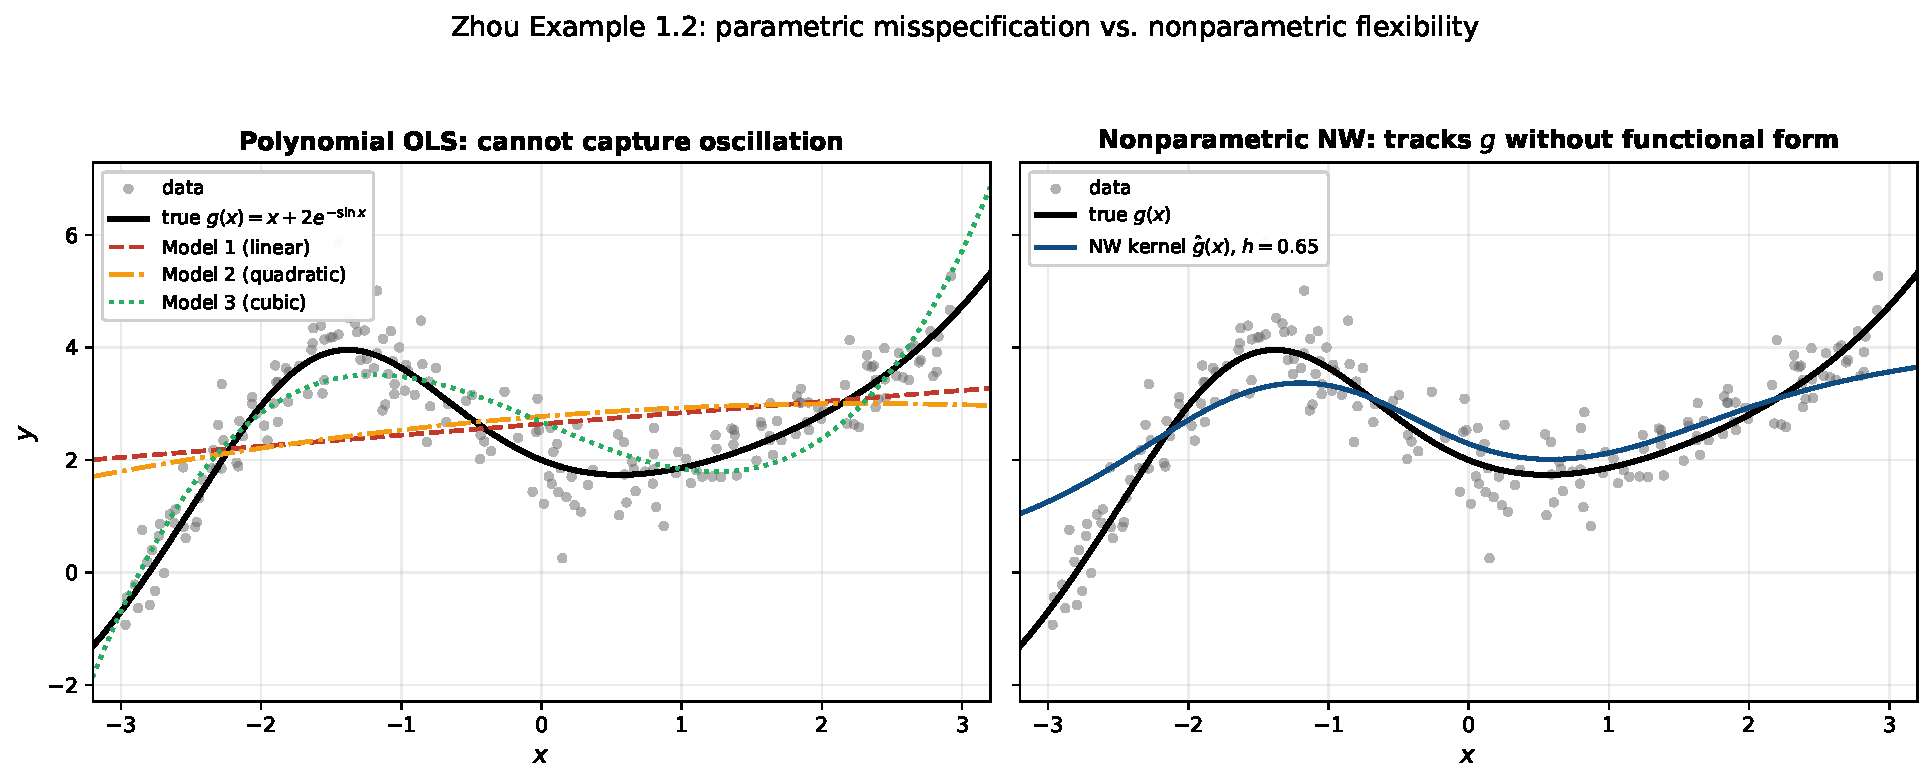
\includegraphics[width=0.95\textwidth]{../Figures/LectureS2/polynomial_misspec.pdf}
  \end{center}

  \begin{keybox}
    \textbf{左图（参数 OLS）}：所有三个多项式拟合都\textbf{无法刻画振荡}——
    Model 1 给出单调直线；Model 2/3 在区间中部勉强近似但尾部严重偏离。
    \quad\textbf{右图（非参数 NW）}：核回归用 Silverman 拇指带宽 $h \approx 0.65$ 紧密追随真实 $g(x)$，
    \textbf{无需事先假设任何函数形式}。
  \end{keybox}

\end{frame}


\begin{frame}{动机四：Li \& Racine——非参数是半参数的基石}

  \begin{columns}[T]
    \begin{column}{0.5\textwidth}
      \begin{keybox}
        \textbf{方法论谱系（Li \& Racine 2007, Ch.1）：}

        \vspace{0.3em}
        \textbf{参数方法}
        \begin{itemize}\footnotesize
          \item 假设强，$\sqrt{n}$ 快
          \item 错了就完全错
        \end{itemize}

        \vspace{0.3em}
        \textbf{半参数方法}（单指标、部分线性）
        \begin{itemize}\footnotesize
          \item $E[Y|X]=G(x'\beta)$，$G$ 未知
          \item $\hat\beta$ 仍 $\sqrt{n}$，$\hat G$ 非参数率
        \end{itemize}

        \vspace{0.3em}
        \textbf{非参数方法}（本讲）
        \begin{itemize}\footnotesize
          \item $E[Y|X]=m(x)$，形式完全未知
          \item 收敛率慢 $n^{-2/(4+d)}$
          \item 是半参数方法的\textbf{必要构件}
        \end{itemize}
      \end{keybox}
    \end{column}
    \begin{column}{0.48\textwidth}
      \begin{highlightbox}
        \textbf{为什么先学非参数？}
        \begin{enumerate}
          \item \textbf{S3 的单指标模型}需要用非参数方法估计链接函数 $G$；
          \item \textbf{Ichimura (1993)} 的 SLS 用核回归估计 $E[Y|x'\beta]$；
          \item \textbf{Klein--Spady (1993)} 的半参数效率界依赖非参数密度估计；
          \item \textbf{规格检验}（Härdle--Mammen, Li--Zheng）比较参数模型与非参数基准。
        \end{enumerate}

        \vspace{0.3em}
        \textbf{三讲一体：}
        \[
          \text{S1 参数} \longrightarrow \text{S2 非参数} \longrightarrow \text{S3 半参数}
        \]
      \end{highlightbox}
    \end{column}
  \end{columns}

\end{frame}


\begin{frame}{本讲路线图}

  \begin{highlightbox}
    \textbf{核心任务：}在\textbf{不假设函数形式}的前提下，估计
    \[
      m(x) = E[Y \mid X = x] \quad\text{以及}\quad f(x) = \text{密度函数}
    \]
  \end{highlightbox}

  \vspace{0.3em}

  \begin{columns}[T]
    \begin{column}{0.48\textwidth}
      \textbf{第一部分（引言）}
      \begin{itemize}\footnotesize
        \item §1 参数方法局限与非参数思想
        \item §2 条件期望与回归函数
      \end{itemize}
      \textbf{第二部分（密度估计）}
      \begin{itemize}\footnotesize
        \item §3 经验分布函数与直方图
        \item §4 核密度估计 (KDE) \ \&\ 窗宽
      \end{itemize}
      \textbf{第三部分（核回归）}
      \begin{itemize}\footnotesize
        \item §5 Nadaraya--Watson 估计量
        \item §6 大样本性质与窗宽选择
      \end{itemize}
      \textbf{第四部分}
      \begin{itemize}\footnotesize
        \item §7 局部多项式估计
      \end{itemize}
    \end{column}
    \begin{column}{0.48\textwidth}
      \textbf{第五部分}
      \begin{itemize}\footnotesize
        \item §8 级数方法（Fourier、Hermite、样条）
      \end{itemize}
      \textbf{第六部分}
      \begin{itemize}\footnotesize
        \item §9 非参数推断（置信区间与 Wild Bootstrap）
      \end{itemize}
      \textbf{第七部分}
      \begin{itemize}\footnotesize
        \item §10 扩展：离散 \& 混合数据核
        \item §11 在二元选择模型中的应用
      \end{itemize}
      \textbf{第八部分}
      \begin{itemize}\footnotesize
        \item §12 总结与 S3 预告
      \end{itemize}
      \textbf{附录}
      \begin{itemize}\footnotesize
        \item 12 个详细证明（proof-b1 $\sim$ proof-b12）
      \end{itemize}
    \end{column}
  \end{columns}

\end{frame}


%% ============================================================
\section{条件数学期望与回归函数的非参数解读}
%% ============================================================

\begin{frame}{条件数学期望的定义}

  \begin{definitionbox}{条件数学期望 (Conditional Expectation)}
    给定随机变量 $Y$ 和 $X$，若 $E[|Y|]<\infty$，则
    \[
      m(x) \;\equiv\; E[Y\mid X=x] \;=\; \int y\, f_{Y\mid X}(y\mid x)\, dy
    \]
    其中 $f_{Y\mid X}(y\mid x) = f_{X,Y}(x,y)/f_X(x)$ 是\textbf{条件密度}。
  \end{definitionbox}

  \textbf{关键性质（全期望律 / Law of Iterated Expectations, LIE）：}
  \[
    E[Y] = E\bigl[E[Y\mid X]\bigr] = \int m(x) f_X(x)\, dx.
  \]

\end{frame}


\begin{frame}{条件数学期望的积分形式}

  \textbf{积分形式（对非参数估计至关重要）：}
  \[
    m(x) = \frac{\int y\, f_{X,Y}(x,y)\, dy}{f_X(x)}
         = \frac{E[Y\cdot \mathds{1}\{X=x\}]}{f_X(x)} \quad\text{(形式记号)}
  \]

  \begin{keybox}
    这个积分形式\textbf{只涉及两个未知物}：联合密度 $f_{X,Y}$ 和边缘密度 $f_X$。
    只要能\textbf{非参数地}估计密度，就能\textbf{非参数地}估计 $m(x)$——这是 NW 估计量的出发点。
  \end{keybox}

\end{frame}


\begin{frame}{回归函数的最优性}

  \begin{highlightbox}
    \textbf{定理（条件期望的最小均方误差性质）：}在所有 $X$ 的可测函数 $g(\cdot)$ 中，$m(x)=E[Y|X=x]$ 是唯一最小化均方预测误差的函数：
    \[
      m(\cdot) \;=\; \arg\min_{g}\; E\bigl[(Y - g(X))^2\bigr].
    \]
  \end{highlightbox}

  \vspace{0.3em}

  \textbf{证明梗概：}分解 $Y-g(X) = [Y-m(X)] + [m(X)-g(X)]$，两项正交（$E\{[Y-m(X)]h(X)\}=0$ 对任意 $h$ 成立），故
  \[
    E[(Y-g(X))^2] = E[(Y-m(X))^2] + E[(m(X)-g(X))^2]
  \]
  \hypertarget{main-b1}{}第一项与 $g$ 无关，第二项取 $g\equiv m$ 时为零。\quad$\square$\ \hfill{\scriptsize\hyperlink{proof-b1}{\beamergotobutton{完整证明}}}


  \begin{keybox}
    \textbf{方法论含义：}
    \begin{itemize}
      \item \textbf{参数方法}（OLS、Probit）事实上解 $\min_\beta E[(Y-x'\beta)^2]$ 或 $\min_\beta E[(Y-\Phi(x'\beta))^2]$；
      \item \textbf{非参数方法}直接对 $m(\cdot)$ 求最优——不对形式设限；
      \item \textbf{正交分解}「偏误 + 方差」的雏形出现在此处——非参数估计的 MSE 分解源自同一思想。
    \end{itemize}
  \end{keybox}

\end{frame}


\begin{frame}{二元响应中的条件概率}

  \begin{keybox}
    \textbf{关键事实：}当 $Y\in\{0,1\}$ 时，
    \[
      E[Y\mid X=x] \;=\; 0\cdot P(Y=0\mid X=x) + 1\cdot P(Y=1\mid X=x) \;=\; P(Y=1\mid X=x).
    \]
    \textbf{估计条件期望 $\equiv$ 估计条件概率。}
  \end{keybox}

  \vspace{0.3em}

  \begin{columns}[T]
    \begin{column}{0.48\textwidth}
      \textbf{参数方法（LectureS1）：}
      \begin{align*}
        P(Y=1\mid X=x) &= \Phi(x'\beta) &\text{Probit}\\
        P(Y=1\mid X=x) &= \Lambda(x'\beta) &\text{Logit}\\
        P(Y=1\mid X=x) &= x'\beta &\text{LPM}
      \end{align*}
      \textbf{代价：}若链接函数错，$\hat\beta$ 不一致。
    \end{column}
    \begin{column}{0.48\textwidth}
      \textbf{非参数方法（本讲）：}
      \[
        P(Y=1\mid X=x) = m(x)
      \]
      形式完全自由——$m(x)$ 可以是 S 形、倒 U 形、分段常数或周期函数。

      \vspace{0.3em}
      \textbf{代价：}收敛率 $n^{-2/(4+d)}$，维数诅咒。
    \end{column}
  \end{columns}

  \begin{highlightbox}
    \textbf{两种范式的权衡：}\textbf{偏误（错设风险）} \,vs.\, \textbf{方差（收敛速度）}。
    半参数方法（S3）尝试在两者之间寻找最优折中。
  \end{highlightbox}

\end{frame}

\begin{frame}{参数与非参数回归的系统对比}
  \centering\small
  \renewcommand{\arraystretch}{1.25}
  \begin{tabular}{@{}p{3.4cm}p{5.0cm}p{5.0cm}@{}}
    \toprule
    \textbf{维度} & \textbf{参数方法} & \textbf{非参数方法} \\
    \midrule
    \textbf{函数形式} & 预先指定（$m(x)=x'\beta$） & 数据驱动（$m(x)$ 未知但光滑） \\
    \textbf{未知量} & 有限维 $\beta\in\mathbb{R}^k$ & 无穷维 $m(\cdot)\in\mathcal{F}$ \\
    \textbf{识别假设} & 强（函数形式正确） & 弱（光滑性 + 矩条件） \\
    \textbf{收敛速度} & $\sqrt{n}$ & $n^{-2/(4+d)}$（$d=\dim X$） \\
    \textbf{渐近分布} & 正态，解析协方差 & 正态（需欠平滑）或 bootstrap \\
    \textbf{可解释性} & 系数即边际效应 & 需计算 $\hat m'(x)$ \\
    \textbf{维数诅咒} & 无 & 有（$d\uparrow\;\Rightarrow$ 率急剧恶化） \\
    \textbf{外推能力} & 可外推到数据支撑外 & 无法外推（需数据附近） \\
    \textbf{计算成本} & 低（一次优化） & 高（每点都是加权平均） \\
    \bottomrule
  \end{tabular}

  \begin{keybox}
    \textbf{黄金法则}（Hansen 2022, Ch.19）：参数方法在\textbf{设定正确}时最优，非参数方法在\textbf{设定未知}时最稳健。实务中常并用：以非参数为「无偏基准」检验参数模型。
  \end{keybox}
\end{frame}


\begin{frame}[shrink=8]{收敛速度的对比：MSE 分解与最优带宽}

  \textbf{两种速度都源于 MSE 分解 $\E[(\hat\theta - \theta)^2] = \text{Bias}^2 + \text{Var}$。}

  \begin{columns}[T]
    \begin{column}{0.5\textwidth}
      \begin{highlightbox}
        \textbf{参数情形（OLS / MLE）：}
        \begin{align*}
          \text{Bias}(\hat\beta) &= 0 \quad (\text{在 MLR 1--4 下}), \\
          \Var(\hat\beta) &= \frac{\sigma^2}{n}\, (\mathbf{X}'\mathbf{X}/n)^{-1}.
        \end{align*}
        $\Rightarrow$ MSE $= O(n^{-1})$，速度 $\sqrt n$.

        \medskip
        关键：模型为\textbf{有限维}（$\dim\beta = k$ 固定），所有 $n$ 个观测值贡献于同一参数估计。
      \end{highlightbox}
    \end{column}
    \begin{column}{0.5\textwidth}
      \begin{highlightbox}
        \textbf{非参数情形（核估计）：}
        \begin{align*}
          \text{Bias}[\hat m(x_0)] &= O(h^2), \\
          \Var[\hat m(x_0)] &= O\!\left(\tfrac{1}{nh^d}\right).
        \end{align*}
        最优 $h^* \propto n^{-1/(4+d)}$ 平衡两项 $\Rightarrow$ MSE $= O(n^{-4/(4+d)})$, 速度 $n^{-2/(4+d)}$.

        \medskip
        关键：$m(x_0)$ 是\textbf{无穷维}对象的局部值，仅 $\approx nh^d$ 个观测落入 $x_0$ 附近的核窗口。
      \end{highlightbox}
    \end{column}
  \end{columns}

  \begin{keybox}
    \textbf{形式化对比：}速度差异不是"几何直觉"，而是 \textbf{Bias-Variance 平衡}的代数结果：
    维度 $d$ 越大，$nh^d$ 越小（窗口内点更稀疏），最优 $h^*$ 必须更慢衰减以控制方差，
    导致剩余偏误项主导，速度恶化。这就是\textbf{维数诅咒}的形式来源。
  \end{keybox}

\end{frame}


\begin{frame}{收敛速度的直觉：等价样本量表}

  \centering\small
  \renewcommand{\arraystretch}{1.2}
  \begin{tabular}{@{}c|cccc@{}}
    \toprule
    维数 $d$ & 收敛率 & $n=100$ 等价参数样本量 & $n=1000$ 等价参数样本量 & $n=10000$ 等价参数样本量 \\
    \midrule
    $1$ & $n^{-2/5}$  & $\approx 6.3$  & $\approx 15.8$  & $\approx 39.8$ \\
    $2$ & $n^{-1/3}$  & $\approx 4.6$  & $\approx 10.0$  & $\approx 21.5$ \\
    $4$ & $n^{-1/4}$  & $\approx 3.2$  & $\approx 5.6$   & $\approx 10.0$ \\
    $8$ & $n^{-1/6}$  & $\approx 2.2$  & $\approx 3.2$   & $\approx 4.6$  \\
    \bottomrule
  \end{tabular}

  \begin{keybox}
    \textbf{维数诅咒 (Curse of Dimensionality, Bellman 1961)：}$d$ 每增加一维，达到同等精度所需样本量指数级增长——这驱动了 S3 中半参数方法（如单指标模型把 $d$ 维问题化约为 1 维）的发展。
  \end{keybox}

\end{frame}


%% %%%%%%%%%%%%%%%%%%%%%%%%%%%%%%%%%%%%%%%%%%%%%%%%%%%%%%%%%%%%
%% 第二部分：密度函数估计
%% %%%%%%%%%%%%%%%%%%%%%%%%%%%%%%%%%%%%%%%%%%%%%%%%%%%%%%%%%%%%

%% ============================================================
\section{经验分布函数与直方图}
%% ============================================================

\begin{frame}{经验分布函数 (Empirical Distribution Function)}

  \begin{definitionbox}{{EDF (Zhou 2013, §2.1)}}
    给定 i.i.d.\ 样本 $\{X_1,\ldots,X_n\}$，\textbf{经验分布函数}定义为
    \[
      \hat F_n(x) \;=\; \frac{1}{n}\sum_{i=1}^n \mathds{1}\{X_i \leq x\}.
    \]
    即「$\leq x$ 的观测所占比例」。
  \end{definitionbox}

  \textbf{EDF 的大样本性质：}
  \begin{enumerate}
    \item \textbf{无偏性}：$E[\hat F_n(x)] = F(x)$（因 $E[\mathds{1}\{X_i\leq x\}]=F(x)$）；
    \item \textbf{相合性}：$\hat F_n(x) \pto F(x)$（LLN）；
    \item \textbf{渐近正态}：$\sqrt{n}[\hat F_n(x)-F(x)] \dto \mathcal{N}(0, F(x)[1-F(x)])$；
    \item \textbf{均匀相合性（Glivenko--Cantelli 定理）：}$\sup_{x}|\hat F_n(x)-F(x)| \overset{\text{a.s.}}{\to} 0$。
  \end{enumerate}

\end{frame}


\begin{frame}{EDF：为什么比密度估计收敛快？}

  \begin{keybox}
    \textbf{EDF 是「分布函数层面」的非参数估计。}它以 $\sqrt{n}$ 速度收敛——\textbf{为什么比密度估计快？}因为 $F(x)$ 是\textbf{积分}过的量（平滑），而 $f(x)=F'(x)$ 需要\textbf{微分}——微分操作放大噪声，因此密度估计本质上更困难。
  \end{keybox}

  \begin{highlightbox}
    \textbf{一般规律：}估计\textbf{积分量}（CDF、矩、分位数）比估计\textbf{微分量}（密度、导数）更易。这个「积分赢，微分输」的模式将贯穿整个非参数理论。
  \end{highlightbox}

\end{frame}


\begin{frame}{从 EDF 到密度：尝试直接微分}

  \begin{highlightbox}
    \textbf{尝试 1：}直接对 $\hat F_n$ 求导得到 $\hat f_n$。
    \[
      \hat f_n(x) \overset{?}{=} \frac{d}{dx}\hat F_n(x).
    \]
    \textbf{问题：}$\hat F_n$ 是\textbf{阶梯函数}（每个 $X_i$ 处跳 $1/n$），导数几乎处处为 $0$，在跳点为 $+\infty$——\textbf{毫无信息}。
  \end{highlightbox}

  \textbf{尝试 2：}用\textbf{有限差分}近似：
  \[
    \hat f_n(x) \approx \frac{\hat F_n(x+h) - \hat F_n(x-h)}{2h}
    = \frac{\#\{X_i \in (x-h, x+h]\}}{2nh}.
  \]

\end{frame}


\begin{frame}{有限差分：窗宽参数 $h$ 的登场}

  \begin{keybox}
    上式正是\textbf{直方图思想}的数学表达：用局部频率近似局部密度。
    引入了一个关键参数 $h$——\textbf{窗宽 (bandwidth)}。
    \begin{itemize}
      \item $h$ 太小 $\Rightarrow$ 窗口内样本少 $\Rightarrow$ 方差大；
      \item $h$ 太大 $\Rightarrow$ 窗口覆盖多种 $x$ $\Rightarrow$ 偏误大。
    \end{itemize}
    \textbf{窗宽选择}将贯穿整个非参数估计理论。
  \end{keybox}

\end{frame}


\begin{frame}{直方图估计量 (Histogram)：定义}

  \begin{definitionbox}{直方图}
    将 $X$ 的取值范围分为若干等宽的\textbf{桶 (bin)}，每个桶宽为 $h$，中心为 $b_j$。
    定义直方图估计量：
    \[
      \hat f_{\text{hist}}(x) \;=\; \frac{1}{nh}\sum_{i=1}^n \mathds{1}\{X_i \in B_j\},\quad \text{其中 } x\in B_j.
    \]
    即「$x$ 所在桶内的样本数 / $(nh)$」。
  \end{definitionbox}

  \textbf{等价表示（指示核）：}$\hat f_{\text{hist}}(x) = \dfrac{1}{nh}\sum_{i=1}^n \mathds{1}\!\left\{\dfrac{X_i-x}{h}\in[-1/2,1/2)\right\}$。

\end{frame}


\begin{frame}{直方图的三个根本缺陷}

  \begin{highlightbox}
    \textbf{直方图的三个根本缺陷（Caetano Class 1, p.3；Zhou §2.2）：}
    \begin{enumerate}
      \item \textbf{同权问题}——\textcolor{negative}{\textit{``there is no reason why we should require that all observations between $x-h$ and $x+h$ have the same weight.''}} 靠近 $x$ 的 $X_i$ 应比远处的 $X_i$ 权重更大；
      \item \textbf{不连续性}——$\hat f_{\text{hist}}$ 在桶边界跳跃，$\hat f'$ 不存在；
      \item \textbf{桶定位敏感}——桶的起点微小平移可能改变形状（众数位置、峰值高度）。
    \end{enumerate}
  \end{highlightbox}

\end{frame}


\begin{frame}{直方图的偏误与方差}

  考虑 $x$ 位于桶 $B_j = [b_j - h/2, b_j + h/2)$ 内的情况。

  \textbf{偏误 (Bias)：}在桶中心做 Taylor 展开，
  \[
    E[\hat f_{\text{hist}}(x)] = \frac{1}{h}\int_{b_j-h/2}^{b_j+h/2} f(u)\, du
    = f(x) + \underbrace{(b_j - x) f'(x) + O(h^2)}_{\text{依赖 }x\text{ 在桶内位置}}.
  \]
  对 $x$ 平均：$\text{Bias}(x) = O(h)$（\textbf{比 KDE 的 }$O(h^2)$\textbf{ 差}）。

  \vspace{0.3em}

  \textbf{方差 (Variance)：}$n_j = \sum_i \mathds{1}\{X_i\in B_j\} \sim \text{Binomial}(n, p_j)$，其中 $p_j \approx h f(b_j)$：
  \[
    \text{Var}[\hat f_{\text{hist}}(x)] = \frac{p_j(1-p_j)}{n^2 h^2} \approx \frac{f(x)}{nh} \quad (h\to 0).
  \]

  \begin{highlightbox}
    \textbf{IMSE（积分均方误）：} $\text{IMSE} = \int[\text{Bias}^2 + \text{Var}]\, dx = O(h^2) + O\!\left(\frac{1}{nh}\right)$.

    \vspace{0.2em}
    最优窗宽：$h^* \propto n^{-1/3}$，最优 IMSE $= O(n^{-2/3})$。

    \vspace{0.3em}
    \textbf{对比 KDE}（下一节）：最优 IMSE $= O(n^{-4/5})$——\textbf{收敛更快}。
    原因：KDE 用光滑核函数消除了桶边界效应，偏误从 $O(h)$ 降为 $O(h^2)$。
  \end{highlightbox}

\end{frame}


%% ============================================================
\section{核密度估计 (Kernel Density Estimation)}
%% ============================================================

\begin{frame}{从直方图到 KDE：Step 1（均匀核重写）}

  \begin{keybox}
    \textbf{思路（Rosenblatt 1956; Parzen 1962）：}用\textbf{光滑权重函数} $K(\cdot)$ 替代直方图的\textbf{硬指示权重}。
  \end{keybox}

  \textbf{Step 1：}直方图可以重写为
  \[
    \hat f_{\text{hist}}(x) = \frac{1}{nh}\sum_{i=1}^n K_0\!\left(\frac{x-X_i}{h}\right),
    \quad K_0(u) = \mathds{1}\{|u|\leq 1/2\}.
  \]
  这里 $K_0$ 是\textbf{均匀核}——在窗口内同权，窗口外零权。

\end{frame}


\begin{frame}{从直方图到 KDE：Step 2（光滑核替换）}

  \textbf{Step 2：}为解决「同权问题」，把 $K_0$ 替换为\textbf{连续光滑}的核函数 $K$，满足：
  \begin{itemize}
    \item $K(u)\geq 0$（非负，保证 $\hat f\geq 0$）；
    \item $\int K(u)\, du = 1$（归一化，保证 $\hat f$ 积分为 1）；
    \item $K(u) = K(-u)$（对称，$\int uK(u)du = 0$）；
    \item $|u|$ 越大 $K(u)$ 越小（远处权重小）。
  \end{itemize}

  \begin{highlightbox}
    \[
      \hat f_h(x) \;=\; \frac{1}{nh}\sum_{i=1}^n K\!\left(\frac{x-X_i}{h}\right).
    \]
    这就是\textbf{核密度估计量 (KDE)}。
  \end{highlightbox}

\end{frame}


\begin{frame}{核函数的形式定义与条件}

  \begin{definitionbox}{{核函数 (Kernel) — Li \& Racine §1.4}}
    函数 $K:\mathbb{R}\to\mathbb{R}$ 是\textbf{二阶核}当满足：
    \begin{align*}
      \text{(K1)} \quad & \int K(u)\, du = 1 && \text{(归一化)}\\
      \text{(K2)} \quad & \int u\, K(u)\, du = 0 && \text{(对称}\Rightarrow\text{一阶矩为零)}\\
      \text{(K3)} \quad & \kappa_2 \;\equiv\; \int u^2 K(u)\, du > 0,\; \text{有限} && \text{(二阶矩存在)}\\
      \text{(K4)} \quad & R(K) \;\equiv\; \int K(u)^2\, du < \infty && \text{(核函数平方可积)}
    \end{align*}
  \end{definitionbox}

\end{frame}


\begin{frame}{核函数条件的经济意义}

  \begin{keybox}
    \textbf{$\kappa_2$ 的作用：}决定 KDE 偏误的常数项——$\text{Bias} = \dfrac{h^2\kappa_2}{2}f''(x) + o(h^2)$。

    \textbf{$R(K)$ 的作用：}决定 KDE 方差的常数项——$\text{Var} = \dfrac{R(K)f(x)}{nh} + o\!\left(\dfrac{1}{nh}\right)$。

    \textbf{高阶核}（$\int u^j K du=0$ for $j=1,\ldots,q-1$, $\int u^q K\neq 0$）可降低偏误至 $O(h^q)$，但会导致 $\hat f$ 可能为负——实务中极少使用。
  \end{keybox}

\end{frame}


\begin{frame}{常用核函数}
  \centering\small
  \renewcommand{\arraystretch}{1.3}
  \begin{tabular}{@{}lllcc@{}}
    \toprule
    \textbf{名称} & \textbf{表达式} $K(u)$ & \textbf{支撑} & $\kappa_2=\int u^2 K$ & $R(K)=\int K^2$ \\
    \midrule
    \textbf{均匀}       & $\tfrac{1}{2}\mathds{1}\{|u|\leq 1\}$ & $[-1,1]$ & $1/3$   & $1/2$ \\
    \textbf{三角}       & $(1-|u|)\mathds{1}\{|u|\leq 1\}$       & $[-1,1]$ & $1/6$   & $2/3$ \\
    \textbf{Epanechnikov}& $\tfrac{3}{4}(1-u^2)\mathds{1}\{|u|\leq 1\}$ & $[-1,1]$ & $1/5$ & $3/5$ \\
    \textbf{双重权}     & $\tfrac{15}{16}(1-u^2)^2\mathds{1}\{|u|\leq 1\}$ & $[-1,1]$ & $1/7$ & $5/7$ \\
    \textbf{三重权}     & $\tfrac{35}{32}(1-u^2)^3\mathds{1}\{|u|\leq 1\}$ & $[-1,1]$ & $1/9$ & $350/429$ \\
    \textbf{高斯}       & $(2\pi)^{-1/2}\exp(-u^2/2)$            & $\mathbb{R}$ & $1$   & $(2\sqrt{\pi})^{-1}$ \\
    \bottomrule
  \end{tabular}


  \begin{keybox}
    \textbf{实用权衡：}
    \begin{itemize}
      \item \textbf{有限支撑}（Epanechnikov、双重权）——计算快，边界清晰；
      \item \textbf{无限支撑}（高斯）——$\hat f$ 光滑到所有阶，但数值慢；
      \item \textbf{光滑度}——双重权比 Epanechnikov 光滑，估计量二阶可导；
      \item 实证中\textbf{核的选择影响小}（< 5\% 效率损失），\textbf{窗宽选择影响大}——先关心 $h$。
    \end{itemize}
  \end{keybox}

\end{frame}


\begin{frame}{Epanechnikov 核的最优性：定理}

  \begin{highlightbox}
    \textbf{定理（Epanechnikov 1969; Hodges--Lehmann 1956）：}在所有满足 (K1)--(K4) 的二阶对称核中，
    \[
      K^*(u) = \frac{3}{4}(1-u^2)\mathds{1}\{|u|\leq 1\}
    \]
    最小化渐近积分均方误 AMISE 的主导常数：$\min_K C(K)$，其中 $C(K) \;=\; \kappa_2^{2/5}\cdot R(K)^{4/5}$.
  \end{highlightbox}

  \textbf{直觉：}\ $\kappa_2$ 控制偏误，$R(K)$ 控制方差——最优核平衡两者。
  Epanechnikov 在约束 $\int K = 1$ 和 $\int u^2 K = \kappa_2$ 下，\textbf{最小化 }$R(K)$（变分法求解）。

  \hypertarget{main-b2}{}\hfill{\scriptsize\hyperlink{proof-b2}{\beamergotobutton{证明}}}

\end{frame}


\begin{frame}{Epanechnikov 核的最优性：相对效率}

  \textbf{相对效率 (relative efficiency)：}若 $K^*_{\text{Ep}}$ 定义效率为 1，其他核的效率为
  \[
    \text{eff}(K) = \frac{C(K^*_{\text{Ep}})}{C(K)}.
  \]
  \small
  \begin{tabular}{@{}lc@{}}
    \toprule
    核                    & 相对效率 \\
    \midrule
    Epanechnikov          & 1.000 \\
    Biweight (Quartic)    & 0.994 \\
    Triweight             & 0.987 \\
    Gaussian              & 0.951 \\
    Uniform               & 0.930 \\
    \bottomrule
  \end{tabular}

  \begin{keybox}
    最大效率损失约 7\%——\textbf{核的选择远不如窗宽选择重要}。Zhou (2013, §2.3) 建议：
    \emph{「窗宽决定质量，核函数决定风格。」}
  \end{keybox}

\end{frame}


\begin{frame}{核密度估计量的正式定义}

  \begin{definitionbox}{{核密度估计量 (Kernel Density Estimator, KDE)}}
    给定 i.i.d.\ 样本 $\{X_1,\ldots,X_n\}\sim f$，核函数 $K$ 满足 (K1)--(K4)，窗宽 $h>0$，\textbf{Rosenblatt--Parzen 估计量}为
    \[
      \boxed{\;\hat f_h(x) \;=\; \frac{1}{nh}\sum_{i=1}^n K\!\left(\frac{x-X_i}{h}\right) \;=\; \frac{1}{n}\sum_{i=1}^n K_h(x-X_i)\;}
    \]
    其中 $K_h(u) \equiv \frac{1}{h}K(u/h)$ 是\textbf{尺度化核}。
  \end{definitionbox}

  \vspace{0.3em}

  \textbf{加权平均解读：}$\hat f_h(x)$ 是 $n$ 个「核包 (kernel bumps)」的平均：
  \begin{itemize}
    \item 每个观测 $X_i$ 贡献一个以 $X_i$ 为中心、宽度 $\propto h$ 的核包 $K_h(\cdot - X_i)/n$；
    \item 观测密集区 $\Rightarrow$ 核包重叠多 $\Rightarrow$ $\hat f$ 大；
    \item 观测稀疏区 $\Rightarrow$ 核包少 $\Rightarrow$ $\hat f$ 小。
  \end{itemize}

\end{frame}


\begin{frame}{KDE 的两个极限情形}

  \begin{keybox}
    \textbf{两个极限情形：}
    \begin{itemize}
      \item $h\to 0$：核包退化为 Dirac 点 $\delta(x-X_i)$，$\hat f_h$ 变成原始数据尖峰——\textbf{过拟合}；
      \item $h\to \infty$：所有核包展平为近常数，$\hat f_h \approx 1/(nh)\sum K(0) \to 0$——\textbf{过平滑}。
    \end{itemize}
    合理的 $h$ 在中间——下面几张幻灯片专注于\textbf{如何选 $h$}。
  \end{keybox}

\end{frame}


\begin{frame}{KDE 偏误的推导：Taylor 展开}

  设 $X_i \overset{\text{iid}}{\sim} f$，$f$ 二阶连续可导。计算
  \[
    E[\hat f_h(x)] = E\!\left[\frac{1}{h}K\!\left(\frac{x-X}{h}\right)\right]
    = \int \frac{1}{h}K\!\left(\frac{x-u}{h}\right) f(u)\, du.
  \]

  \textbf{换元} $u = x - hv$，$du = -h\,dv$：
  \[
    E[\hat f_h(x)] = \int K(v) f(x - hv)\, dv.
  \]

  \textbf{Taylor 展开} $f(x-hv) = f(x) - hv f'(x) + \tfrac{(hv)^2}{2}f''(x) + o(h^2)$ 并代入：
  \begin{align*}
    E[\hat f_h(x)]
    &= f(x)\underbrace{\int K(v)dv}_{=1} - hf'(x)\underbrace{\int vK(v)dv}_{=0} \\
    &\quad + \tfrac{h^2}{2}f''(x)\underbrace{\int v^2 K(v)dv}_{=\kappa_2} + o(h^2).
  \end{align*}

\end{frame}


\begin{frame}{KDE 偏误的结果与解读}

  \begin{highlightbox}
    \[
      \boxed{\;\text{Bias}[\hat f_h(x)] = \tfrac{h^2}{2}\kappa_2\, f''(x) + o(h^2).\;}
    \]
    \textbf{解读：}
    \begin{itemize}
      \item 偏误与 $h^2$ 成正比——$h\uparrow$ $\Rightarrow$ 偏误大；
      \item 偏误与 $f''(x)$ 成正比——曲率大处（峰、谷）偏误最严重；
      \item 在 $f''>0$（U 形）处向上偏，$f''<0$（倒 U）处向下偏——\textbf{峰值被压平，谷值被抬高}。
    \end{itemize}
  \end{highlightbox}
  \hypertarget{main-b3}{}\hfill{\scriptsize\hyperlink{proof-b3}{\beamergotobutton{附录证明}}}

\end{frame}


\begin{frame}{KDE 方差的推导}

  \[
    \text{Var}[\hat f_h(x)] = \frac{1}{n}\text{Var}\!\left[\frac{1}{h}K\!\left(\frac{x-X}{h}\right)\right]
    = \frac{1}{n}\left\{E\!\left[\frac{1}{h^2}K^2\!\left(\tfrac{x-X}{h}\right)\right] - \bigl(E[\cdots]\bigr)^2\right\}.
  \]

  \textbf{主项：}（换元 $v = (x-u)/h$）
  \[
    E\!\left[\frac{1}{h^2}K^2\!\left(\frac{x-X}{h}\right)\right]
    = \frac{1}{h}\int K^2(v) f(x-hv)\, dv
    = \frac{f(x)}{h}\int K^2(v)\, dv + O(1).
  \]

  次项 $(E[\cdots])^2 = (f(x)+O(h^2))^2 = O(1)$，与主项 $O(1/h)$ 相比可忽略。

  \begin{highlightbox}
    \[
      \boxed{\;\text{Var}[\hat f_h(x)] = \frac{R(K)\, f(x)}{nh} + o\!\left(\frac{1}{nh}\right).\;}
    \]
    \textbf{解读：}
    \begin{itemize}
      \item 方差与 $(nh)^{-1}$ 成正比——\textbf{有效样本量} $nh\to\infty$ 方差才消失；
      \item 方差与 $f(x)$ 成正比——密度高处估计更精确（更多邻近观测）；
      \item 方差与 $R(K)$ 成正比——「粗糙」的核方差更大。
    \end{itemize}
  \end{highlightbox}

\end{frame}


\begin{frame}{MSE 与 IMSE：从逐点到积分}

  \textbf{逐点均方误差 (Pointwise MSE)：}
  \[
    \text{MSE}(x) = \text{Bias}^2 + \text{Var}
    = \frac{h^4}{4}\kappa_2^2 [f''(x)]^2 + \frac{R(K)f(x)}{nh} + o(h^4) + o\!\left(\frac{1}{nh}\right).
  \]

  \textbf{积分均方误差 (IMSE)：}对 $x$ 积分，
  \[
    \text{IMSE}(h) = \int \text{MSE}(x)\, dx
    = \frac{h^4}{4}\kappa_2^2 R(f'') + \frac{R(K)}{nh} + \text{高阶项},
  \]
  其中 $R(f'') = \int [f''(x)]^2 dx$ 是密度二阶导数的 $L^2$ \textbf{范数平方}，衡量密度的\textbf{振荡程度}（密度曲线越陡峭、波动越多，$R(f'')$ 越大）。

\end{frame}


\begin{frame}{AMISE 与偏误--方差权衡}

  \begin{highlightbox}
    \textbf{渐近 IMSE (AMISE)：}
    \[
      \boxed{\;\text{AMISE}(h) = \underbrace{\frac{h^4}{4}\kappa_2^2 R(f'')}_{\text{偏误}^2} + \underbrace{\frac{R(K)}{nh}}_{\text{方差}}\;}
    \]
    \textbf{偏误--方差权衡}在此处以\textbf{完全解析}的形式呈现：
    \begin{itemize}
      \item $h\uparrow$ $\Rightarrow$ 偏误项 $\uparrow$，方差项 $\downarrow$；
      \item $h\downarrow$ $\Rightarrow$ 偏误项 $\downarrow$，方差项 $\uparrow$；
      \item \textbf{最优 $h^*$} 使两项平衡——见下一张幻灯片。
    \end{itemize}
  \end{highlightbox}

\end{frame}


\begin{frame}{最优窗宽的推导与 $n^{-1/5}$ 速率}

  \textbf{一阶条件}：对 AMISE$(h)$ 求 $h$ 的导数并令为零：
  \[
    \frac{d}{dh}\text{AMISE}(h) = h^3 \kappa_2^2 R(f'') - \frac{R(K)}{nh^2} = 0.
  \]

  \textbf{解得}：
  \[
    \boxed{\;h^*_{\text{AMISE}} = \left[\frac{R(K)}{\kappa_2^2 R(f'')}\right]^{1/5} n^{-1/5}.\;}
  \]

  \textbf{代入 AMISE}：
  \[
    \text{AMISE}(h^*) = \frac{5}{4}\left[\kappa_2^2 R(f'') R(K)^4\right]^{1/5} n^{-4/5}.
  \]

  \begin{keybox}
    \textbf{三个关键含义：}
    \begin{enumerate}
      \item \textbf{最优窗宽速率} $h^*\propto n^{-1/5}$——$n$ 越大，$h^*$ 越小（核包越窄）；
      \item \textbf{最优 IMSE 速率} $n^{-4/5}$——\textbf{比参数 $n^{-1}$ 慢}，但是可达的最快非参数速率；
      \item \textbf{实际不可用}：$h^*$ 依赖未知的 $R(f'')$——需要实用替代方案。
    \end{enumerate}
  \end{keybox}
  \hypertarget{main-b7}{}\hfill{\scriptsize\hyperlink{proof-b7}{\beamergotobutton{附录详细推导}}}

\end{frame}


\begin{frame}{Silverman 拇指法则：思路与推导}

  \textbf{思路}（Silverman 1986）：\textbf{假设} $f$ 是 $\mathcal{N}(\mu,\sigma^2)$，计算 $R(f'')$ 的解析值：
  \[
    R(f'') = \int [f''(x)]^2 dx = \frac{3}{8\sqrt{\pi}\, \sigma^5}.
  \]

  \textbf{代入最优窗宽公式}（高斯核 $\kappa_2=1$，$R(K) = 1/(2\sqrt{\pi})$）：
  \[
    h^*_{\text{Normal}} = \left[\frac{4}{3}\right]^{1/5} \sigma n^{-1/5} \approx 1.06\, \sigma\, n^{-1/5}.
  \]

\end{frame}


\begin{frame}{Silverman 拇指法则 (ROT)：定义与优劣}

  \begin{definitionbox}{Silverman 拇指法则 (ROT)}
    \[
      \boxed{\; \hat h_{\text{ROT}} = 1.06 \cdot \min\!\left\{\hat\sigma,\, \frac{\text{IQR}}{1.34}\right\} \cdot n^{-1/5}.\;}
    \]
    其中 $\hat\sigma$ 是样本标准差，IQR 是四分位距，$1.34$ 是标准正态 IQR。取 min 使法则对厚尾/偏态更稳健。
  \end{definitionbox}

  \begin{keybox}
    \textbf{优点：}极简单，无需迭代；实务中常作为其他方法的\textbf{初始值}。

    \textbf{缺点：}若真实 $f$ 远离正态（多峰、厚尾、非对称），$\hat h_{\text{ROT}}$ \textbf{系统性过大}——倾向\textbf{过平滑}。Zhou (§2.4) 将此称为「正态参考法的危险」。
  \end{keybox}

\end{frame}


\begin{frame}{插入法 (Plug-In Bandwidth)：两阶段构造}

  \textbf{思路（Sheather \& Jones 1991）}：既然 $h^*$ 依赖未知 $R(f'')$，就\textbf{非参数地}估计 $R(f'')$，再「插入」公式。

  \begin{definitionbox}{两阶段插入法}
    \textbf{Stage 1：}用\textbf{先导窗宽} $g$ 估计 $\hat f''_{g}(x)$，得
    \[
      \widehat{R(f'')} = \int [\hat f''_g(x)]^2 dx.
    \]
    \textbf{Stage 2：}代入最优窗宽公式，
    \[
      \hat h_{\text{PI}} = \left[\frac{R(K)}{\kappa_2^2\,\widehat{R(f'')}}\right]^{1/5} n^{-1/5}.
    \]
  \end{definitionbox}

  \textbf{Sheather--Jones 方法}使用迭代求解保证 $g = g(h)$ 一致。

\end{frame}


\begin{frame}{插入法：性质与软件实现}

  \begin{keybox}
    \textbf{性质（Sheather 2004）：}
    \begin{itemize}
      \item \textbf{理论最优：}$\hat h_{\text{PI}}/h^* \pto 1$，\textbf{渐近一致}；
      \item \textbf{实务表现：}在双峰、偏态分布下明显优于 ROT；
      \item \textbf{软件实现：}R 中 \texttt{bw.SJ()}；Stata 中 \texttt{kdensity, bwidth(sj)}；Python 中 \texttt{statsmodels.nonparametric.KDEUnivariate}；
      \item \textbf{推荐：}Sheather--Jones 插入法是实务\textbf{首选}。
    \end{itemize}
  \end{keybox}

\end{frame}


\begin{frame}{最小二乘交叉鉴定法 (LSCV)：推导}

  \textbf{思路（Rudemo 1982; Bowman 1984）}：直接最小化 IMSE 的样本估计。

  \textbf{IMSE 展开：}
  \[
    \text{IMSE}(h) = E\!\int [\hat f_h(x) - f(x)]^2 dx
    = E\!\int \hat f_h^2 - 2E\!\int \hat f_h f + \int f^2.
  \]
  第三项 $\int f^2$ 与 $h$ 无关。第一项直接计算：$\int \hat f_h^2 dx$。第二项用\textbf{留一法 (leave-one-out)}估计：
  \[
    E\!\int \hat f_h(x) f(x) dx = E[\hat f_h(X)] \approx \frac{1}{n}\sum_{i=1}^n \hat f_{h,-i}(X_i),
  \]
  其中 $\hat f_{h,-i}(x) = \frac{1}{(n-1)h}\sum_{j\neq i} K\!\left(\frac{x-X_j}{h}\right)$。

\end{frame}


\begin{frame}{LSCV：定义与性质}

  \begin{definitionbox}{最小二乘交叉鉴定法 (LSCV)}
    \[
      \boxed{\; \text{CV}(h) = \int \hat f_h^2(x)\, dx - \frac{2}{n}\sum_{i=1}^n \hat f_{h,-i}(X_i),\quad \hat h_{\text{LSCV}} = \arg\min_h \text{CV}(h).\;}
    \]
  \end{definitionbox}

  \begin{keybox}
    \textbf{性质：}数据驱动、通用（无分布假设）、$\hat h_{\text{LSCV}}/h^*\pto 1$。
    \textbf{缺点：}CV 函数常呈\textbf{多峰}，$\hat h_{\text{LSCV}}$ 方差大——实务中波动较剧烈。
  \end{keybox}

\end{frame}


\begin{frame}{窗宽选择方法的对比}
  \centering\small
  \renewcommand{\arraystretch}{1.3}
  \begin{tabular}{@{}p{3.0cm}p{3.5cm}p{3.5cm}p{3.3cm}@{}}
    \toprule
    \textbf{特性} & \textbf{Silverman ROT} & \textbf{插入法 (SJ)} & \textbf{LSCV} \\
    \midrule
    计算成本 & 一次性，$O(n)$ & 中等，需迭代 & 需网格搜索 \\
    对 $f$ 的假设 & 正态参考 & 无（非参数 $\hat f''$） & 无 \\
    偏好 & \textbf{过平滑} & 平衡 & 略\textbf{欠平滑} \\
    稳定性 & 很稳定 & 稳定 & 方差大 \\
    一致性 & 若 $f$ 非正态则\textbf{不一致} & 一致 $\hat h/h^*\pto 1$ & 一致 $\hat h/h^*\pto 1$ \\
    实务推荐 & 初始值/快速预览 & \textbf{首选} & 交叉验证；二选 \\
    R 函数 & \texttt{bw.nrd0} & \texttt{bw.SJ} & \texttt{bw.ucv} \\
    \bottomrule
  \end{tabular}


  \begin{keybox}
    \textbf{Zhou (2013, §2.5) 实务建议：}
    \begin{enumerate}
      \item 先用 ROT 看「大致形状」；
      \item 用 SJ 插入法作为\textbf{正式报告}的窗宽；
      \item 用 LSCV 做\textbf{稳健性检查}——两种方法差异大提示样本存在非标准结构（多峰、厚尾）；
      \item 对数据做变换后再估计（如对右偏数据取对数）也是常见策略。
    \end{enumerate}
  \end{keybox}

\end{frame}


\begin{frame}{KDE 的相合性与渐近正态性}

  \begin{assumptionbox}
    \textbf{（KDE-1）}$\{X_i\}$ 是 i.i.d.\ 样本，真实密度 $f$ 二阶连续可导。\\
    \textbf{（KDE-2）}核 $K$ 满足 (K1)--(K4)。\\
    \textbf{（KDE-3）}窗宽 $h = h_n$ 满足 $h\to 0$ 且 $nh\to\infty$。
  \end{assumptionbox}

  \begin{highlightbox}
    \textbf{定理 1（逐点相合性）：}在 (KDE-1)--(KDE-3) 下，$\hat f_h(x) \pto f(x)$。

    \textbf{证明梗概：}$E[\hat f_h(x)]\to f(x)$（偏误 $=O(h^2)\to 0$），$\text{Var}[\hat f_h(x)]\to 0$（$=O(1/nh)\to 0$）。由 MSE 相合即可。

    \textbf{定理 2（渐近正态性）：}若另假设 $nh^5\to C\in[0,\infty)$，
    \[
      \sqrt{nh}\left[\hat f_h(x) - f(x) - \tfrac{h^2}{2}\kappa_2 f''(x)\right]
      \dto \mathcal{N}\!\left(0,\; R(K) f(x)\right).
    \]
  \end{highlightbox}

\end{frame}


\begin{frame}{KDE 渐近：偏误不消失的两个对策}

  \begin{keybox}
    \textbf{偏误不消失！}在最优窗宽下（$h\propto n^{-1/5}$，$nh^5\to C>0$），偏误项\textbf{与方差同阶}，不可忽略。
    这带来两个实务选项：
    \begin{itemize}
      \item \textbf{欠平滑 (undersmoothing)}：选 $h = o(n^{-1/5})$，使偏误项 $\sqrt{nh}\cdot h^2 \to 0$；
      \item \textbf{偏误校正}：估计 $\hat f''$ 并减去偏误——构造置信区间时常用。
    \end{itemize}
  \end{keybox}

\end{frame}


%% %%%%%%%%%%%%%%%%%%%%%%%%%%%%%%%%%%%%%%%%%%%%%%%%%%%%%%%%%%%%
%% 第三部分：核回归估计 (Nadaraya--Watson)
%% %%%%%%%%%%%%%%%%%%%%%%%%%%%%%%%%%%%%%%%%%%%%%%%%%%%%%%%%%%%%

%% ============================================================
\section{Nadaraya--Watson 核回归估计量}
%% ============================================================

\begin{frame}{从条件期望到核回归：策略与 Step 1}

  回忆 \S2 的基本关系：
  \[
    m(x) = E[Y\mid X=x] = \frac{\int y\, f_{X,Y}(x,y)\, dy}{f_X(x)}.
  \]

  \textbf{策略（Nadaraya 1964; Watson 1964）：}用\textbf{核估计量}分别替换分子与分母的密度。

  \textbf{Step 1：}对联合密度 $f_{X,Y}(x,y)$ 使用二维乘积核：
  \[
    \hat f_{X,Y}(x,y) = \frac{1}{nh_x h_y}\sum_{i=1}^n K\!\left(\frac{x-X_i}{h_x}\right) K\!\left(\frac{y-Y_i}{h_y}\right).
  \]

\end{frame}


\begin{frame}{从条件期望到核回归：Step 2--3}

  \textbf{Step 2：}计算\textbf{分子}——对 $y$ 积分（关键：用\emph{零矩性质} $\int y K((y-Y_i)/h_y)dy = h_y Y_i$）：
  \[
    \int y\, \hat f_{X,Y}(x,y)\, dy = \frac{1}{nh_x}\sum_{i=1}^n K\!\left(\frac{x-X_i}{h_x}\right) Y_i.
  \]

  \textbf{Step 3：}\textbf{分母}是 $\hat f_X(x) = \frac{1}{nh_x}\sum_i K((x-X_i)/h_x)$。\textbf{两者相除}：
  \[
    \boxed{\;\hat m_{\text{NW}}(x) = \dfrac{\displaystyle\sum_{i=1}^n K_h(x-X_i)\, Y_i}{\displaystyle\sum_{i=1}^n K_h(x-X_i)}.\;}
  \]

\end{frame}


\begin{frame}{NW 估计量的正式定义}

  \begin{definitionbox}{Nadaraya--Watson 估计量}
    给定 i.i.d.\ 样本 $\{(X_i, Y_i)\}_{i=1}^n$，核 $K$ 满足 (K1)--(K4)，窗宽 $h>0$：
    \[
      \hat m_{\text{NW}}(x) \;=\; \frac{\sum_{i=1}^n K\!\left(\frac{x-X_i}{h}\right) Y_i}{\sum_{i=1}^n K\!\left(\frac{x-X_i}{h}\right)}
      \;=\; \sum_{i=1}^n w_i(x)\, Y_i
    \]
    其中\textbf{局部权重}为
    \[
      w_i(x) = \frac{K_h(x-X_i)}{\sum_{j=1}^n K_h(x-X_j)},\qquad \sum_{i=1}^n w_i(x) = 1.
    \]
  \end{definitionbox}

\end{frame}


\begin{frame}{NW 估计量：三个解读视角}

  \begin{keybox}
    \textbf{三个解读：}
    \begin{enumerate}
      \item \textbf{局部加权平均}——$\hat m_{\text{NW}}(x)$ 是 $\{Y_i\}$ 的凸组合，权重由 $X_i$ 与 $x$ 的距离决定；
      \item \textbf{局部常数拟合}——下一页显示 NW 等价于「在 $x$ 处用 WLS 拟合常数」；
      \item \textbf{数据驱动}——完全无需假设 $m(\cdot)$ 的函数形式。
    \end{enumerate}
  \end{keybox}

\end{frame}


\begin{frame}{NW 作为局部常数加权最小二乘 (LCLS)}

  \textbf{等价优化问题：}在点 $x$ 处，求 $\alpha$ 最小化\textbf{局部加权 SSR}：
  \[
    \hat\alpha(x) = \arg\min_{\alpha\in\mathbb{R}} \sum_{i=1}^n K_h(x-X_i)\bigl[Y_i - \alpha\bigr]^2.
  \]

  \textbf{一阶条件：} $\dfrac{\partial}{\partial\alpha} = -2\sum_i K_h(x-X_i)[Y_i - \alpha] = 0$，解得
  \[
    \hat\alpha(x) = \frac{\sum_i K_h(x-X_i) Y_i}{\sum_i K_h(x-X_i)} = \hat m_{\text{NW}}(x).
  \]

  \begin{highlightbox}
    \textbf{关键视角：}NW = \textbf{局部常数拟合}。在每一点 $x$，用距离 $x$ 近的样本拟合一个\textbf{水平线 $\alpha$}，该水平线即为 $\hat m_{\text{NW}}(x)$。

    \vspace{0.3em}
    这一视角为\textbf{局部多项式估计}（\S7）做了铺垫：若把「局部常数」替换为「局部线性」或「局部二次」，就得到\textbf{Fan \& Gijbels (1996)} 的局部多项式估计量——它在边界处表现更优。
  \end{highlightbox}

\end{frame}


\begin{frame}{NW 估计量的正则性假设}
  \begin{assumptionbox}
    \textbf{（NW-1）样本}：$\{(X_i,Y_i)\}_{i=1}^n$ 为 i.i.d.\ 样本；$E[Y^2]<\infty$。\\
    \textbf{（NW-2）回归函数}：$m(x) = E[Y\mid X=x]$ 二阶连续可导。\\
    \textbf{（NW-3）密度}：$X$ 的密度 $f_X$ 二阶连续可导，在 $x$ 处 $f_X(x)>0$。\\
    \textbf{（NW-4）条件方差}：$\sigma^2(x) = \text{Var}(Y\mid X=x)$ 在 $x$ 附近连续。\\
    \textbf{（NW-5）核}：$K$ 满足 (K1)--(K4)（二阶、对称）。\\
    \textbf{（NW-6）窗宽}：$h = h_n$，$h\to 0$，$nh\to\infty$。\\
    \textbf{（NW-7）矩条件}：$E[|Y|^{2+\delta}\mid X=x] < \infty$ 对某 $\delta>0$（用于 CLT）。\\
    \textbf{（NW-8）等变差序列条件}：针对时间序列数据推广时添加。
  \end{assumptionbox}

  \begin{keybox}
    这些条件比参数方法严——\textbf{非参数方法换取更弱的函数形式假设，代价是更强的光滑性和矩条件}。实务中 $f_X(x) > 0$ 是\textbf{边界问题}的根源：在 $X$ 分布尾部 $f_X$ 很小，NW 的方差爆炸。
  \end{keybox}
\end{frame}


\begin{frame}{NW 偏误：分子与分母的 Taylor 展开}

  分子 $\hat m_1(x) = \frac{1}{nh}\sum_i K_h(x-X_i) Y_i$，分母 $\hat f_X(x)$。用 $Y_i = m(X_i) + u_i$，$E[u_i|X_i]=0$：
  \[
    E[\hat m_1(x)] = E\!\left[\frac{1}{h}K\!\left(\frac{x-X}{h}\right) m(X)\right]
    = \int K(v) m(x-hv) f_X(x-hv)\, dv.
  \]

  \textbf{Taylor 展开}（设 $\varphi(u) = m(u)f_X(u)$）：
  \[
    \varphi(x-hv) = \varphi(x) - hv\varphi'(x) + \tfrac{h^2 v^2}{2}\varphi''(x) + o(h^2).
  \]
  代入并使用 $\int K = 1$，$\int vK = 0$，$\int v^2 K = \kappa_2$：
  \[
    E[\hat m_1(x)] = \varphi(x) + \tfrac{h^2 \kappa_2}{2}\varphi''(x) + o(h^2).
  \]
  类似 $E[\hat f_X(x)] = f_X(x) + \tfrac{h^2\kappa_2}{2}f_X''(x) + o(h^2)$。

\end{frame}


\begin{frame}{NW 偏误：比率偏误公式}

  \begin{highlightbox}
    \textbf{比率偏误（一阶近似）：}
    \[
      \boxed{\;\text{Bias}[\hat m_{\text{NW}}(x)]
      = \frac{h^2 \kappa_2}{2}\left[m''(x) + 2\,\frac{m'(x) f_X'(x)}{f_X(x)}\right] + o(h^2).\;}
    \]
    \textbf{注意括号内的第二项}——设计密度项 $\frac{m'f_X'}{f_X}$。在 $f_X$ 急剧变化处（分布尾部），NW 偏误被放大。\textbf{局部线性估计量将消除这一项}（\S7）。
  \end{highlightbox}
  \hypertarget{main-b4}{}\hfill{\scriptsize\hyperlink{proof-b4}{\beamergotobutton{完整推导}}}

\end{frame}


\begin{frame}{NW 方差的推导}

  类似 KDE 方差推导，主项来自 $\text{Var}\!\left[\frac{1}{nh}\sum K_h(x-X_i) Y_i\right]$ 的 $O(1/nh)$ 部分。
  使用分解 $Y = m(X) + u$ 并注意 $\text{Var}(u\mid X) = \sigma^2(X)$，可推出：
  \[
    \text{Var}[\hat m_{\text{NW}}(x)] = \frac{R(K)\, \sigma^2(x)}{nh\, f_X(x)} + o\!\left(\frac{1}{nh}\right).
  \]

  \begin{highlightbox}
    \[
      \boxed{\;\text{Var}[\hat m_{\text{NW}}(x)] = \frac{R(K)\, \sigma^2(x)}{nh\, f_X(x)} + o\!\left(\frac{1}{nh}\right).\;}
    \]
    \textbf{三个关键因素：}
    \begin{itemize}
      \item \textbf{分子 $\sigma^2(x)$}——条件方差大处估计噪声大；
      \item \textbf{分母 $f_X(x)$}——密度低处（尾部）方差爆炸——这是非参数方法\textbf{外推能力差}的直接原因；
      \item \textbf{分母 $nh$}——\textbf{有效样本量}，在点 $x$ 附近约有 $nh f_X(x)$ 个「有效观测」。
    \end{itemize}
  \end{highlightbox}

\end{frame}


\begin{frame}{NW 的相合性定理}

  \begin{highlightbox}
    \textbf{定理 3（NW 逐点相合性）：}在 (NW-1)--(NW-6) 下，若 $f_X(x)>0$，则
    \[
      \hat m_{\text{NW}}(x) \pto m(x).
    \]
  \end{highlightbox}

  \vspace{0.3em}

  \hypertarget{main-b8}{}\textbf{证明梗概：}由 $\text{MSE} = \text{Bias}^2 + \text{Var} = O(h^4) + O(1/nh) \to 0$，故 $\hat m_{\text{NW}}(x) \to m(x)$ 于 $L^2$，因而亦 in probability。\quad$\square$\ \hfill{\scriptsize\hyperlink{proof-b8}{\beamergotobutton{附录}}}


  \begin{keybox}
    \textbf{相合性的\emph{率}}：由最优偏误--方差权衡，取 $h^* \propto n^{-1/5}$，得
    \[
      |\hat m_{\text{NW}}(x) - m(x)| = O_p(n^{-2/5}).
    \]
    这比参数方法的 $O_p(n^{-1/2})$ \textbf{慢}——但\textbf{无函数形式偏误}。

    \vspace{0.3em}
    在多维情形 $d\geq 2$：$h^* \propto n^{-1/(4+d)}$，$|\hat m - m| = O_p(n^{-2/(4+d)})$——\textbf{维数诅咒}显现。
  \end{keybox}

\end{frame}


\begin{frame}{NW 的渐近正态性}

  \begin{highlightbox}
    \textbf{定理 4（Nadaraya--Watson CLT）：}在 (NW-1)--(NW-7) 下，若 $nh^5 \to C\in[0,\infty)$，
    \[
      \sqrt{nh}\Bigl[\hat m_{\text{NW}}(x) - m(x) - B_{\text{NW}}(x) h^2\Bigr]
      \;\dto\; \mathcal{N}\!\left(0,\; V_{\text{NW}}(x)\right),
    \]
    其中
    \[
      B_{\text{NW}}(x) = \tfrac{\kappa_2}{2}\left[m''(x) + 2\tfrac{m'(x) f_X'(x)}{f_X(x)}\right],\qquad
      V_{\text{NW}}(x) = \tfrac{R(K)\sigma^2(x)}{f_X(x)}.
    \]
  \end{highlightbox}

  \vspace{0.3em}

  \textbf{收敛率：}$\sqrt{nh}$——比参数 $\sqrt{n}$ \textbf{慢}，等价于只有 $nh$ 个「有效观测」。

  \textbf{在最优 $h = O(n^{-1/5})$ 下：}$\sqrt{nh}\cdot h^2 = n^{2/5}\cdot n^{-2/5} = O(1)$——\textbf{偏误项 $B h^2$ 不消失}，需欠平滑或偏误校正才能做置信区间。

  \begin{keybox}
    \textbf{与 KDE CLT 的完全对应：}结构相同（$\sqrt{nh}$ 速率、$h^2$ 偏误、$R(K)$ 与 $f_X$ 进入方差），只是把「$f$」换成了「$m$」、把「$f(x)$」换成了「$\sigma^2(x)/f_X(x)$」。
  \end{keybox}
  \hypertarget{main-b5}{}\hfill{\scriptsize\hyperlink{proof-b5}{\beamergotobutton{证明}}}

\end{frame}


\begin{frame}{NW 最优窗宽 (AMSE 最优)}

  \textbf{逐点 AMSE：}
  \[
    \text{AMSE}(x; h) = B_{\text{NW}}(x)^2 h^4 + \frac{V_{\text{NW}}(x)}{nh}.
  \]

  \textbf{一阶条件}对 $h$ 求导：$4 B^2 h^3 - V/(nh^2) = 0$，解得
  \[
    h^*_{\text{NW}}(x) = \left[\frac{V_{\text{NW}}(x)}{4 B_{\text{NW}}(x)^2}\right]^{1/5} n^{-1/5}.
  \]

  \textbf{全局 AMISE 最优窗宽}（对 $x$ 积分加权）：
  \[
    h^*_{\text{global}} = \left[\frac{R(K)\int \sigma^2(x) w(x) dx}{\kappa_2^2 \int \bigl(m''(x) + 2 m'(x) f_X'(x)/f_X(x)\bigr)^2 f_X^2(x) w(x) dx}\right]^{1/5} n^{-1/5}.
  \]

  \begin{keybox}
    \textbf{与 KDE 的类比：}结构类似，但涉及\textbf{两个未知函数} $m$ 和 $f_X$ 及其导数——\textbf{回归问题比密度估计更复杂}。
    故实务中常用\textbf{数据驱动}的交叉验证而不是插入法。
  \end{keybox}

\end{frame}


\begin{frame}{回归的 LSCV：留一法推导}

  \textbf{预测误差目标：}
  \[
    \text{APE}(h) = E\left[(Y - \hat m_{h}(X))^2\right].
  \]

  \textbf{留一法估计：}
  \[
    \boxed{\;\text{CV}(h) = \frac{1}{n}\sum_{i=1}^n \bigl[Y_i - \hat m_{h,-i}(X_i)\bigr]^2,\;}
  \]
  其中 $\hat m_{h,-i}(X_i) = \dfrac{\sum_{j\neq i} K_h(X_i - X_j) Y_j}{\sum_{j\neq i} K_h(X_i - X_j)}$。

  \begin{highlightbox}
    \textbf{留一法的必要性：}若使用全样本，$X_i$ 在 $\hat m_h(X_i)$ 的分母与分子中都占主导（$K_h(0)$ 最大），导致\textbf{过拟合}——CV 在 $h\to 0$ 时趋于 0，失去选择能力。
  \end{highlightbox}

\end{frame}


\begin{frame}{回归 LSCV：性质与软件}

  \begin{keybox}
    \textbf{性质（Härdle--Marron 1985）：}
    \begin{itemize}
      \item LSCV 是 AMISE 的\textbf{渐近无偏}估计；
      \item $\hat h_{\text{LSCV}}/h^*_{\text{AMISE}} \pto 1$——一致；
      \item CV 函数常\textbf{多峰}——需全局网格搜索；
      \item R 函数：\texttt{np::npreg()} 自动 LSCV；\texttt{locpol::regCVBwSelC()}。
    \end{itemize}
  \end{keybox}

\end{frame}


\begin{frame}{边界偏误问题 (Boundary Bias)}

  \textbf{问题：}在 $X$ 支撑的\textbf{边界点}附近（如 $x = x_{\min} + h$），核权重$K_h(x-X_i)$ 只能使用「单边」样本：
  \[
    \text{Bias}[\hat m_{\text{NW}}(x_{\text{boundary}})] = O(h)\quad \text{不再是 }O(h^2).
  \]

  \begin{highlightbox}
    \textbf{为什么是 $O(h)$ 而不是 $O(h^2)$？}

    \vspace{0.2em}
    内点处：$\int vK(v)dv = 0$（对称核），\textbf{一阶项消失}，偏误从 $h^2$ 开始。

    边界处：积分区间不对称（如 $[0, 1]$ 变成 $[-1, 0]$），$\int_{\text{截断}} vK(v)dv \neq 0$——\textbf{一阶项不消失}，偏误退化为 $h$ 阶。
  \end{highlightbox}

  \vspace{0.3em}

  \textbf{后果：}在经济应用中，常要估计\textbf{分布边缘的效应}（最低收入者、最高年龄段、政策阈值附近）——正是边界偏误最严重之处。

  \begin{keybox}
    \textbf{解决方案（按复杂度递增）：}
    \begin{enumerate}
      \item 忽略边界（只在内部报告）——简单但浪费数据；
      \item \textbf{边界核}——修改 $K$ 使其在截断区间保持零阶矩；
      \item \textbf{局部线性估计}（\S7）——\textbf{自动}把偏误降回 $O(h^2)$，这是最优方案；
      \item \textbf{映射变换}——对 $X$ 做映射使支撑为 $\mathbb{R}$（如对正变量取对数）。
    \end{enumerate}
  \end{keybox}

\end{frame}


\begin{frame}{多元 NW：乘积核}

  \textbf{多元回归：}$X = (X^{(1)},\ldots,X^{(d)})\in\mathbb{R}^d$。

  \begin{definitionbox}{乘积核 (Product Kernel)}
    使用每一维单独的核：
    \[
      K\!\left(\frac{x-X_i}{\mathbf{h}}\right) = \prod_{\ell=1}^d K\!\left(\frac{x^{(\ell)} - X_i^{(\ell)}}{h_\ell}\right).
    \]
    多元 NW 估计量：
    \[
      \hat m_{\text{NW}}(x) = \frac{\sum_i \prod_\ell K\!\left(\frac{x^{(\ell)}-X_i^{(\ell)}}{h_\ell}\right) Y_i}{\sum_i \prod_\ell K\!\left(\frac{x^{(\ell)}-X_i^{(\ell)}}{h_\ell}\right)}.
    \]
  \end{definitionbox}

  \textbf{窗宽向量}：$\mathbf{h} = (h_1, \ldots, h_d)$，可每维不同；实务常用\textbf{标准化}让 $h_\ell \propto \hat\sigma_\ell \cdot h$。

\end{frame}


\begin{frame}{乘积核 vs.\ 球形核}

  \begin{keybox}
    \textbf{乘积核 vs.\ 球形核}：
    \begin{itemize}
      \item \textbf{乘积核}——计算快，实务首选；各维窗宽可分别选；
      \item \textbf{球形核}（如多元 Epanechnikov $K(\|u\|)$）——各向同性，但窗宽选择困难；
      \item 两者的渐近性质\textbf{相同阶}——区别仅在常数；
      \item \textbf{各向异性带宽矩阵}推广：$\mathbf{H}$ 为正定矩阵，$K_\mathbf{H}(u)= |\mathbf{H}|^{-1/2}K(\mathbf{H}^{-1/2}u)$，可处理相关协变量——Wand \& Jones (1995, Ch.4)。
    \end{itemize}
  \end{keybox}

\end{frame}


\begin{frame}{维数诅咒：收敛率恶化}

  \textbf{多元 NW 的 AMSE：}
  \[
    \text{AMSE}(x) = O(h^4) + O\!\left(\frac{1}{n h^d}\right).
  \]
  平衡两项：$h^* \propto n^{-1/(4+d)}$，最优 $\text{AMSE}^* = O(n^{-4/(4+d)})$。

  \centering\small
  \renewcommand{\arraystretch}{1.2}
  \begin{tabular}{@{}ccccc@{}}
    \toprule
    $d$ & $h^* \propto$ & $\text{MSE}^* \propto$ & \multicolumn{2}{c}{达到 $\text{MSE}=0.01$ 所需 $n$} \\
        &              &                        & 参数 ($n^{-1}$)   & 非参数 \\
    \midrule
    1 & $n^{-1/5}$  & $n^{-4/5}$  & 100        & 178      \\
    2 & $n^{-1/6}$  & $n^{-2/3}$  & 100        & 1{,}000   \\
    3 & $n^{-1/7}$  & $n^{-4/7}$  & 100        & 3{,}981   \\
    5 & $n^{-1/9}$  & $n^{-4/9}$  & 100        & 27{,}826  \\
    10 & $n^{-1/14}$ & $n^{-2/7}$  & 100        & $1.85\times 10^6$ \\
    \bottomrule
  \end{tabular}

  \begin{highlightbox}
    \textbf{Bellman (1961) 的维数诅咒：}$d$ 每增加 1，所需样本量\textbf{几何级增长}。经济应用中 $d=5\sim 10$ 常见，这使得\textbf{纯非参数回归实际上不可行}——必须限制结构（单指标、可加性、部分线性）。
  \end{highlightbox}

\end{frame}


\begin{frame}{维数诅咒的几何直觉：球面现象}

  \begin{keybox}
    \textbf{高维球面现象：}$\mathbb{R}^d$ 中单位球的体积
    \[
      V_d = \frac{\pi^{d/2}}{\Gamma(d/2+1)}
      \xrightarrow{d\to\infty} 0.
    \]
    高维单位球的\textbf{体积几乎为 0}——数据在高维空间中\textbf{极为稀疏}。
  \end{keybox}

  \textbf{直观示例：}若要在 $[0,1]^d$ 中覆盖 10\% 的体积（「$x$ 附近的邻域」），所需立方体边长：
  \small
  \begin{center}
  \begin{tabular}{@{}c|c@{}}
    \toprule
    $d$ & 边长 $= 0.1^{1/d}$ \\
    \midrule
    1 & 0.10 \\
    2 & 0.32 \\
    5 & 0.63 \\
    10 & 0.79 \\
    20 & 0.89 \\
    \bottomrule
  \end{tabular}
  \end{center}
  \normalsize

\end{frame}


\begin{frame}{维数诅咒：结构假设的必要性}

  即\textbf{$d=10$ 时要覆盖 10\% 体积需要近 80\% 的边长}——「局部」已变「全局」，核回归本质上退化为\textbf{全局参数回归}。

  \begin{highlightbox}
    这解释了为什么\textbf{没有任何方法能「纯非参数地」解决高维问题}——必须引入\textbf{结构假设}（单指标、可加性、稀疏性）。\textbf{半参数方法（S3）由此而生。}
  \end{highlightbox}

  \begin{keybox}
    \textbf{三类常用结构假设}（按约束强度递增）：
    \begin{itemize}
      \item \textbf{可加性}（additive）：$m(x) = \sum_\ell m_\ell(x_\ell)$；
      \item \textbf{部分线性}：$m(x) = z'\gamma + m_0(x_0)$；
      \item \textbf{单指标}：$m(x) = G(x'\beta)$——\textbf{S3 重点}。
    \end{itemize}
  \end{keybox}

\end{frame}


\begin{frame}{应对维数诅咒 (1/2)：加性与部分线性}

  \begin{highlightbox}
    \textbf{三大策略，按约束强度递增。}
  \end{highlightbox}

  \textbf{策略 1：加性模型 (Additive Model; Stone 1985)}
  \[
    m(x_1,\ldots,x_d) = c_0 + \sum_{\ell=1}^d m_\ell(x_\ell).
  \]
  每个 $m_\ell$ 以 \textbf{单维率} $n^{-2/5}$ 估计——摆脱维数诅咒。

  \textbf{策略 2：部分线性模型 (Robinson 1988)}
  \[
    Y_i = Z_i'\gamma + m(X_i) + u_i,\quad m\in\mathcal{F}.
  \]
  $\gamma$ 以 $\sqrt{n}$ 率估计，$m$ 以非参数率。

\end{frame}


\begin{frame}{应对维数诅咒 (2/2)：单指标——走向 S3}

  \textbf{策略 3：单指标模型 (Ichimura 1993; Klein--Spady 1993)}
  \[
    E[Y\mid X=x] = G(x'\beta),\quad G \text{ 未知}.
  \]
  $\beta$ 以 $\sqrt{n}$ 率估计，$G$ 以 1 维非参数率——\textbf{把 }$d$\textbf{ 维问题化约为 1 维}。

  \begin{keybox}
    \textbf{S3 的核心：}单指标模型是二元选择非参数化的最自然扩展——保留 Probit/Logit 的 $x'\beta$ 结构，但释放链接函数的形式。
  \end{keybox}

\end{frame}


%% %%%%%%%%%%%%%%%%%%%%%%%%%%%%%%%%%%%%%%%%%%%%%%%%%%%%%%%%%%%%
%% 第四部分：局部多项式估计
%% %%%%%%%%%%%%%%%%%%%%%%%%%%%%%%%%%%%%%%%%%%%%%%%%%%%%%%%%%%%%

%% ============================================================
\section{局部多项式估计 (Local Polynomial Regression)}
%% ============================================================

\begin{frame}{从局部常数到局部多项式：动机}

  \textbf{NW 的局限（回顾）：}
  \begin{itemize}
    \item 偏误含设计密度项 $2 m'(x) f_X'(x)/f_X(x)$；
    \item 边界处偏误退化为 $O(h)$。
  \end{itemize}

  \begin{keybox}
    \textbf{Fan \& Gijbels (1996) 的洞见：}
    NW 在 $x$ 附近用\textbf{常数}近似 $m$——这丢失了\textbf{一阶信息}（斜率）。若改用\textbf{局部线性}近似
    \[
      m(X_i) \approx m(x) + m'(x)(X_i - x),
    \]
    偏误就能自动消去 $m'$ 相关的一阶效应。
  \end{keybox}

  \vspace{0.3em}

  \textbf{思路：}在每一点 $x$ 处，对 $m$ 做 \textbf{$p$ 阶 Taylor 展开}，用加权最小二乘估计展开系数。
  \[
    m(X_i) \approx \beta_0 + \beta_1(X_i - x) + \cdots + \tfrac{1}{p!}\beta_p(X_i - x)^p.
  \]
  $\hat\beta_0$ 即为 $\hat m(x)$；$\hat\beta_1$ 即为 $\hat m'(x)$（\textbf{免费得到导数估计}！）。

\end{frame}


\begin{frame}{局部多项式估计量的定义}

  \begin{definitionbox}{局部 $p$ 阶多项式估计 (Local Polynomial of Order $p$)}
    在点 $x$ 处，求 $\boldsymbol{\beta}(x) = (\beta_0, \beta_1, \ldots, \beta_p)'$ 最小化加权 SSR：
    \[
      \hat{\boldsymbol{\beta}}(x) = \arg\min_{\boldsymbol{\beta}} \sum_{i=1}^n K_h(x - X_i)\left[Y_i - \sum_{j=0}^p \beta_j (X_i - x)^j\right]^2.
    \]
    估计量：$\hat m_{\text{LP}(p)}(x) = \hat\beta_0(x)$；$\hat m^{(r)}_{\text{LP}(p)}(x) = r!\, \hat\beta_r(x)$。
  \end{definitionbox}

  \vspace{0.3em}

  \textbf{特殊情形：}
  \begin{itemize}
    \item $p=0$：\textbf{局部常数} = Nadaraya--Watson；
    \item $p=1$：\textbf{局部线性} (LL) —— Fan \& Gijbels 推荐的\textbf{默认选择}；
    \item $p=2$：\textbf{局部二次} (LQ) —— 用于估计 $m''$ 或复杂曲率；
    \item $p$ 偶数 $\Rightarrow$ $p+1$ 奇数：可进一步降低内点偏误阶——\textbf{奇阶多项式占优 (odd-order wins)}。
  \end{itemize}

\end{frame}


\begin{frame}{局部多项式估计：矩阵形式}

  \textbf{记号：}$\mathbf{X}_x$ 为 $n\times(p+1)$ 设计矩阵：
  \[
    \mathbf{X}_x = \begin{pmatrix}
      1 & (X_1-x) & \cdots & (X_1-x)^p \\
      \vdots & \vdots & & \vdots \\
      1 & (X_n-x) & \cdots & (X_n-x)^p
    \end{pmatrix},\quad
    \mathbf{W}_x = \text{diag}\{K_h(x-X_1),\ldots,K_h(x-X_n)\}.
  \]

  \textbf{WLS 解：}
  \[
    \boxed{\;\hat{\boldsymbol{\beta}}(x) = (\mathbf{X}_x'\mathbf{W}_x \mathbf{X}_x)^{-1}\mathbf{X}_x'\mathbf{W}_x \mathbf{Y}.\;}
  \]

  \textbf{抽取第 0 个分量：}$\hat m(x) = \mathbf{e}_0'(\mathbf{X}_x'\mathbf{W}_x \mathbf{X}_x)^{-1}\mathbf{X}_x'\mathbf{W}_x \mathbf{Y}$，其中 $\mathbf{e}_0 = (1,0,\ldots,0)'$。

  \begin{keybox}
    \textbf{等价权重形式：}$\hat m(x) = \sum_{i=1}^n \ell_i(x; h) Y_i$，其中
    \[
      \ell_i(x;h) = \mathbf{e}_0'(\mathbf{X}_x'\mathbf{W}_x \mathbf{X}_x)^{-1}(1, X_i-x, \ldots, (X_i-x)^p)'\cdot K_h(x-X_i).
    \]
    故局部多项式估计也是\textbf{线性平滑器 (linear smoother)}——理论性质与 NW 可类比。
  \end{keybox}

\end{frame}


\begin{frame}{局部线性估计：局部矩定义}

  \textbf{$p=1$ 情形}。定义局部矩：
  \[
    S_j(x) = \frac{1}{n}\sum_{i=1}^n K_h(x-X_i)(X_i-x)^j,\qquad j=0,1,2.
  \]
  \[
    T_j(x) = \frac{1}{n}\sum_{i=1}^n K_h(x-X_i)(X_i-x)^j Y_i,\qquad j=0,1.
  \]

  \textbf{使用这些局部矩，局部线性估计量可以写成封闭形式}——见下一张幻灯片。

\end{frame}


\begin{frame}{局部线性估计：显式公式}

  \begin{definitionbox}{{局部线性估计量 (Local Linear, LL)}}
    \[
      \hat m_{\text{LL}}(x) = \frac{S_2(x) T_0(x) - S_1(x) T_1(x)}{S_0(x) S_2(x) - S_1(x)^2}.
    \]
    等价地：
    \[
      \hat m_{\text{LL}}(x) = \sum_{i=1}^n \ell_i^{\text{LL}}(x) Y_i,\quad
      \ell_i^{\text{LL}}(x) = \frac{[S_2(x) - S_1(x)(X_i-x)] K_h(x-X_i)}{n[S_0(x) S_2(x) - S_1(x)^2]}.
    \]
  \end{definitionbox}

  \begin{keybox}
    \textbf{实用观察：}当 $f_X$ 对称时 $S_1 \approx 0$，LL 几乎退化为 NW；当 $f_X$ 不对称时（或在边界），$S_1 \ne 0$ 产生\textbf{设计偏误修正}——这是 LL 优越性的数学根源。
  \end{keybox}

\end{frame}


\begin{frame}{LL 对比 NW：偏误的对比}

  \begin{highlightbox}
    \textbf{内点 ($x$ 离边界远)：}
    \begin{align*}
      \text{Bias}[\hat m_{\text{NW}}(x)] &= \frac{h^2\kappa_2}{2}\left[m''(x) + 2\frac{m'(x)f_X'(x)}{f_X(x)}\right] + o(h^2), \\
      \text{Bias}[\hat m_{\text{LL}}(x)] &= \frac{h^2\kappa_2}{2}\, m''(x) + o(h^2).
    \end{align*}
  \end{highlightbox}

  \begin{keybox}
    \textbf{关键差异：}LL 偏误\textbf{不含设计密度项}！
    \begin{itemize}
      \item NW 偏误在 $f_X$ 急剧变化处（尾部、多峰谷底）被放大；
      \item LL 偏误只依赖 $m''$——\textbf{「设计自适应 (design-adaptive)」}（Fan 1992）；
      \item 方差两者相同：$\text{Var}[\hat m_{\text{LL}}(x)] = R(K)\sigma^2(x)/(nhf_X(x))$；
      \item \textbf{LL 弱占优 NW}——偏误更小（或相等），方差相同。
    \end{itemize}
  \end{keybox}

  \vspace{0.3em}
  \textbf{结论：}实务\textbf{默认}选择局部线性 (LL) 而非 NW——「同等方差下的更小偏误」几乎是「免费午餐」。

\end{frame}


\begin{frame}{LL 对比 NW：边界处的决定性优势}

  \textbf{边界点（$x$ 在支撑边缘）：}
  \[
    \text{Bias}[\hat m_{\text{NW}}(x_{\text{bd}})] = O(h),\qquad
    \text{Bias}[\hat m_{\text{LL}}(x_{\text{bd}})] = O(h^2).
  \]

  \begin{highlightbox}
    \textbf{LL 自动解决边界问题！}
    \vspace{0.2em}

    原因：LL 在每一点\textbf{显式拟合截距 + 斜率}。即使样本「只在一侧」，回归直线也能合理外推到 $x$ 处——无需对核作特殊处理。
  \end{highlightbox}


  \begin{keybox}
    \textbf{实证启示：}
    \begin{itemize}
      \item \textbf{RDD（回归断点）}：断点处本质是边界问题——\textbf{Imbens \& Kalyanaraman (2012)、Calonico--Cattaneo--Titiunik (2014)} 的 RD 带宽理论全部基于 LL 估计；
      \item \textbf{分位回归端点}：在 $\tau$ 接近 0 或 1 时，LL 修正「稀疏尾部」偏误；
      \item \textbf{生存分析}：在寿命分布截断处，LL 给出无偏残存率估计。
    \end{itemize}
  \end{keybox}

\end{frame}


\begin{frame}{局部二次与更高阶多项式}

  \textbf{偏误阶（内点, $p$ 阶局部多项式）：}
  \begin{itemize}
    \item $p=0$ (NW): Bias $= O(h^2)$；
    \item $p=1$ (LL): Bias $= O(h^2)$，但无设计偏误；
    \item $p=2$ (LQ): Bias $= O(h^4)$？—— \textbf{不，仍是 $O(h^2)$}；
    \item $p=3$ (LC, local cubic): Bias $= O(h^4)$。
  \end{itemize}

  \begin{highlightbox}
    \textbf{奇阶多项式占优定理 (Fan \& Gijbels 1996, Thm 3.1)：}
    只有当 $p$ 从偶数增加到奇数时，偏误阶才降低。这是因为\textbf{对称核下高阶奇矩为零}——奇数阶多项式的额外项不增加方差。
  \end{highlightbox}


  \begin{keybox}
    \textbf{实务推荐：}
    \begin{itemize}
      \item \textbf{估计 $m$ 本身} $\Rightarrow$ 用 LL ($p=1$)——简单、稳健、无设计偏误；
      \item \textbf{估计导数 $m^{(r)}$} $\Rightarrow$ 用 $p=r+1$ 或 $p=r+3$ 阶多项式；
      \item $p\geq 3$ 的额外收益通常被方差增加抵消——\textbf{$p=1$ 是实际应用中的首选}。
    \end{itemize}
  \end{keybox}

\end{frame}


\begin{frame}{局部线性的渐近正态性}

  \begin{highlightbox}
    \textbf{定理 5（LL CLT, Fan \& Gijbels 1996）：}在 NW 类似假设下，
    \[
      \sqrt{nh}\Bigl[\hat m_{\text{LL}}(x) - m(x) - B_{\text{LL}}(x) h^2\Bigr]
      \dto \mathcal{N}\!\left(0,\; V_{\text{LL}}(x)\right),
    \]
    其中
    \[
      B_{\text{LL}}(x) = \tfrac{\kappa_2}{2}\, m''(x),\qquad
      V_{\text{LL}}(x) = \tfrac{R(K)\sigma^2(x)}{f_X(x)}.
    \]
  \end{highlightbox}

  \vspace{0.3em}

  \textbf{与 NW 对比：}
  \begin{center}\small
  \begin{tabular}{@{}lcc@{}}
    \toprule
     & NW & LL \\
    \midrule
    偏误常数 & $\tfrac{\kappa_2}{2}[m'' + 2 m' f'/f]$ & $\tfrac{\kappa_2}{2} m''$ \\
    方差常数 & $R(K)\sigma^2/f$ & $R(K)\sigma^2/f$ \\
    边界偏误 & $O(h)$ & $O(h^2)$ \\
    \bottomrule
  \end{tabular}
  \end{center}

  \begin{keybox}
    \textbf{$\sqrt{nh}$ 收敛率不变}——LL 相对于 NW 是\textbf{偏误的改进}，不是收敛率的改进。
    要改进收敛率必须假设更多光滑性（使用更高阶多项式）。
  \end{keybox}
  \hypertarget{main-b6}{}\hfill{\scriptsize\hyperlink{proof-b6}{\beamergotobutton{证明}}}

\end{frame}


\begin{frame}{局部多项式：窗宽选择与实用建议}

  \textbf{窗宽选择方法（同 NW 可推广）：}
  \begin{itemize}
    \item \textbf{LSCV}：$\text{CV}(h) = n^{-1}\sum_i [Y_i - \hat m_{\text{LL},-i}(X_i)]^2$；
    \item \textbf{插入法}：$\hat h = \left[R(K)\hat V/(\kappa_2^2\widehat{\int(m'')^2 f_X^2 w})\right]^{1/5} n^{-1/5}$——Ruppert--Sheather--Wand (1995)；
    \item \textbf{自适应窗宽}：在 $x$ 处用本地方差选 $h(x)$——\textbf{Cattaneo} 等人的「MSE-optimal local bandwidth」。
  \end{itemize}


  \begin{highlightbox}
    \textbf{方法对比表：}
  \end{highlightbox}
  \centering\small
  \renewcommand{\arraystretch}{1.25}
  \begin{tabular}{@{}llccc@{}}
    \toprule
    方法 & 估计方程 & 内点偏误阶 & 边界偏误阶 & 设计自适应 \\
    \midrule
    NW (LC) & $\min_\alpha \sum w_i(Y_i-\alpha)^2$ & $h^2$ & $h$ & 否 \\
    LL      & $\min_{\alpha,\beta} \sum w_i(Y_i-\alpha-\beta(X_i-x))^2$ & $h^2$ & $h^2$ & \textbf{是} \\
    LQ      & LL + $(X_i-x)^2$ 项 & $h^2$ & $h^2$ & 是 \\
    LC      & LQ + $(X_i-x)^3$ 项 & $h^4$ & $h^4$ & 是 \\
    \bottomrule
  \end{tabular}

  \begin{keybox}
    \textbf{Zhou (§3.3) 与 Hansen (Ch.19) 一致建议：}\textbf{默认使用 LL}。若需导数估计或 RDD 分析，则考虑更高阶（奇数阶）局部多项式。
  \end{keybox}

\end{frame}


%% %%%%%%%%%%%%%%%%%%%%%%%%%%%%%%%%%%%%%%%%%%%%%%%%%%%%%%%%%%%%
%% 第五部分：级数方法
%% %%%%%%%%%%%%%%%%%%%%%%%%%%%%%%%%%%%%%%%%%%%%%%%%%%%%%%%%%%%%

%% ============================================================
\section{级数方法 (Series Methods)}
%% ============================================================

\begin{frame}[shrink=8]{为什么需要级数方法？——核方法的局限}

  迄今为止讨论的核方法（KDE, NW, 局部多项式）虽然形式简单，但在以下场景下不够：

  \begin{highlightbox}
    \textbf{核方法面临的六大限制：}
    \begin{enumerate}\setlength{\itemsep}{2pt}
      \item \textbf{维数诅咒}：核估计速率 $n^{-2/(4+d)}$ 在 $d \geq 3$ 几乎不可行；级数方法利用\textbf{光滑度} $s$ 达到 $n^{-2s/(2s+d)}$，对高维更友好。
      \item \textbf{导数估计}：级数方法的导数 $\hat m^{(r)}(x) = \sum_k \hat\beta_k p_k^{(r)}(x)$ 只需对基函数求导，简单且光滑；核导数估计噪声极大。
      \item \textbf{结构约束}：易在基函数选择层面施加\textbf{单调性、凸性、加法可分性}（如 $m(x) = \sum_l g_l(x_l)$）；核方法很难。
      \item \textbf{计算简单}：级数估计本质是\textbf{对变换后回归元的 OLS}——无需选择带宽与核，无边界修正。
      \item \textbf{半参数效率}：级数估计与 $\sqrt{n}$ 一致估计的参数部分（如部分线性模型、IV 回归）天然兼容，效率界推导清晰。
      \item \textbf{边界行为}：核估计在边界处偏误 $O(h)$（内部 $O(h^2)$）；级数方法（尤其多项式与样条）\textbf{自然处理边界}，无需额外修正。
    \end{enumerate}
  \end{highlightbox}

  \begin{keybox}
    \textbf{核心权衡：}级数方法用\textbf{基函数选择}（替代带宽选择）+\textbf{阶数 $K$ 选择}（替代核选择）换取上述优势。本部分推导级数估计量、阶数选择（Mallows $C_L$、GCV、LOOCV）、与核方法的精确对比。
  \end{keybox}

\end{frame}

\begin{frame}{级数方法的基本思想}

  \begin{keybox}
    \textbf{出发点：}若 $m(x)$ 属于某函数空间 $\mathcal{F}$，它可以被\textbf{基函数 $\{p_k(x)\}$ 的线性组合}逼近：
    \[
      m(x) \approx \sum_{k=0}^{K} c_k\, p_k(x),\qquad K\to\infty\text{ 时近似误差 }\to 0.
    \]
  \end{keybox}

  \vspace{0.3em}

  \textbf{常见基函数：}
  \begin{itemize}
    \item \textbf{幂级数 (Power Series)}：$p_k(x) = x^k$——简单但数值不稳定（高阶幂之间相关性高，导致设计矩阵接近奇异）；
    \item \textbf{Fourier 基}：$p_k(x) = \sin(k\pi x), \cos(k\pi x)$——周期函数逼近；
    \item \textbf{多项式正交基}：Legendre、Chebyshev、Hermite——数值稳定；
    \item \textbf{样条 (Splines)}：B-spline、自然样条——局部支撑，节点灵活；
    \item \textbf{小波 (Wavelets)}：Haar、Daubechies——多尺度分析。
  \end{itemize}

  \textbf{关键参数：}\textbf{项数} $K$——核方法中的「窗宽」的类比。$K$ 太小偏误大，$K$ 太大方差大。

\end{frame}


\begin{frame}{级数回归估计量：定义}

  \begin{definitionbox}{级数估计量 (Sieve / Series Estimator)}
    选定基 $\{p_k\}_{k=0}^K$，定义 $n\times(K+1)$ 设计矩阵
    \[
      \mathbf{P} = \begin{pmatrix}
        p_0(X_1) & p_1(X_1) & \cdots & p_K(X_1) \\
        \vdots & & & \vdots \\
        p_0(X_n) & p_1(X_n) & \cdots & p_K(X_n)
      \end{pmatrix}.
    \]
    \textbf{OLS}：
    \[
      \hat{\boldsymbol{c}} = (\mathbf{P}'\mathbf{P})^{-1} \mathbf{P}' \mathbf{Y},\qquad
      \hat m(x) = \sum_{k=0}^K \hat c_k p_k(x) = p(x)'\hat{\boldsymbol{c}}.
    \]
  \end{definitionbox}

\end{frame}


\begin{frame}{级数估计：相对核方法的优劣}

  \begin{keybox}
    \textbf{优势（相比核方法）：}
    \begin{itemize}
      \item \textbf{计算简单}——只是一次 OLS；
      \item \textbf{全局光滑}——无需逐点迭代；
      \item \textbf{高维自然推广}——张量积基 $p_{k_1}(x_1)\cdots p_{k_d}(x_d)$；
      \item \textbf{标准工具箱}——$t$ 检验、$F$ 检验、VCE 都可用。
    \end{itemize}

    \textbf{劣势：}项数 $K$ 选择复杂、基函数选择影响大、局部性差。
  \end{keybox}

\end{frame}


\begin{frame}{Fourier 基与幂级数}

  \begin{definitionbox}{{Fourier 基（周期函数, $[0, 2\pi]$）}}
    \[
      p_{2k-1}(x) = \sin(kx),\quad p_{2k}(x) = \cos(kx),\quad k=1,2,\ldots.
    \]
    \textbf{正交性}：$\int_0^{2\pi} \sin(kx)\sin(jx) dx = \pi \delta_{jk}$（$k\neq 0$）。
  \end{definitionbox}

  \begin{definitionbox}{幂级数（支撑任意）}
    \[
      p_k(x) = x^k,\quad k=0,1,2,\ldots,K.
    \]
  \end{definitionbox}

  \begin{highlightbox}
    \textbf{幂级数的数值缺陷：}设计矩阵 $\mathbf{P}$ 的\textbf{条件数随 $K$ 指数级增长}——$(\mathbf{P}'\mathbf{P})^{-1}$ 数值不稳定。
    \vspace{0.2em}

    \textbf{解决方案：}
    \begin{itemize}
      \item 先\textbf{标准化} $X$ 到 $[-1,1]$；
      \item 用\textbf{正交多项式}（Chebyshev、Legendre）代替原始幂次；
      \item 使用样条而非多项式——\textbf{局部基函数}避免全局相关性。
    \end{itemize}
  \end{highlightbox}

\end{frame}


\begin{frame}{Hermite 多项式基：定义}

  \begin{definitionbox}{Hermite 多项式 (Probabilists' Convention)}
    Hermite 多项式 $H_k(x)$ 定义为：
    \[
      H_k(x) = (-1)^k \phi(x)^{-1} \frac{d^k}{dx^k}\phi(x),
    \]
    其中 $\phi(x) = (2\pi)^{-1/2}\exp(-x^2/2)$ 是标准正态密度。

    \textbf{前几阶：}$H_0(x) = 1$，$H_1(x) = x$，$H_2(x) = x^2 - 1$，$H_3(x) = x^3 - 3x$。

    \textbf{正交性（以 $\phi$ 为权）：}
    \[
      \int_{-\infty}^{\infty} H_j(x) H_k(x) \phi(x)\, dx = k!\, \delta_{jk}.
    \]
  \end{definitionbox}

\end{frame}


\begin{frame}{Hermite 多项式基：实证优势}

  \begin{keybox}
    \textbf{Hermite 基的优势（Zhou §4.4）：}
    \begin{itemize}
      \item \textbf{支撑 $\mathbb{R}$}——适合\textbf{无界变量}（收入、资产等）；
      \item \textbf{对正态权测度正交}——系数估计方差解析；
      \item \textbf{密度估计}：若真实密度 $f = \phi \cdot \exp(\sum c_k H_k)$，Hermite 级数\textbf{保证非负性}；
      \item \textbf{Gallant--Nychka (1987) SNP 方法}：用 Hermite 基做准则函数估计半参数模型；
      \item \textbf{Fenton--Gallant (1996)}：Hermite 级数可近似任意连续密度。
    \end{itemize}
  \end{keybox}

\end{frame}


\begin{frame}{B-样条基}

  \begin{definitionbox}{B-样条 (B-splines)}
    给定\textbf{节点序列} $\xi_0 < \xi_1 < \cdots < \xi_J$，$d$ 阶 B-样条基 $B_{k,d}(x)$ 由 Cox--de Boor 递推定义：
    \[
      B_{k,0}(x) = \mathds{1}\{x\in[\xi_k, \xi_{k+1})\},
    \]
    \[
      B_{k,d}(x) = \frac{x-\xi_k}{\xi_{k+d}-\xi_k} B_{k,d-1}(x) + \frac{\xi_{k+d+1}-x}{\xi_{k+d+1}-\xi_{k+1}} B_{k+1,d-1}(x).
    \]
  \end{definitionbox}

  \vspace{0.3em}

  \textbf{特点：}
  \begin{itemize}
    \item \textbf{局部支撑}——$B_{k,d}$ 仅在 $d+2$ 个相邻节点区间内非零 $\Rightarrow$ 设计矩阵\textbf{带状}（稀疏），计算 $O(n)$ 而非 $O(n K)$；
    \item \textbf{光滑度}——$d$ 阶 B-样条是 $d-1$ 阶连续可导（$d=3$ 最常用 = 三次样条）；
    \item \textbf{形状灵活}——节点可\textbf{等距}或\textbf{分位数等样本密度}分布。
  \end{itemize}

  \begin{keybox}
    \textbf{实务推荐：}三次 B-样条（$d=3$）+ 分位数节点是\textbf{级数方法首选}——兼顾光滑度、局部性、计算速度。R 包 \texttt{splines::bs()}。
  \end{keybox}

\end{frame}


\begin{frame}{项数 $K$ 选择：Mallows $C_L$ 准则}

  \textbf{目标：}最小化 $\text{APE}(K) = E[(Y - \hat m_K(X))^2]$。

  \begin{definitionbox}{Mallows $C_L$ 准则 (Mallows 1973)}
    \[
      C_L(K) = \text{SSR}(K) + 2 K \hat\sigma^2,\qquad \text{SSR}(K) = \sum_{i=1}^n [Y_i - \hat m_K(X_i)]^2.
    \]
    其中 $\hat\sigma^2$ 是\textbf{全局}残差方差（通常用最大 $K$ 的模型估计）。
    \[
      \hat K_{\text{Mallows}} = \arg\min_K C_L(K).
    \]
  \end{definitionbox}

  \textbf{直觉：}第一项 SSR 衡量\textbf{拟合优度}（$K\uparrow$ 递减），第二项 $2K\hat\sigma^2$ 惩罚\textbf{复杂度}。

\end{frame}


\begin{frame}{$K$ 选择：$C_L$ 与 AIC/BIC 的关系}

  \begin{keybox}
    \textbf{相关准则：}
    \begin{itemize}
      \item \textbf{AIC}：$\text{SSR}(K) + 2K\hat\sigma^2$（与 $C_L$ 几乎相同）；
      \item \textbf{BIC}：$\text{SSR}(K) + \log(n)\cdot K\hat\sigma^2$（更重惩罚 $\Rightarrow$ 更小 $K$ $\Rightarrow$ 一致选择「真」模型）；
      \item \textbf{选 AIC 做预测，选 BIC 做解释}——经验法则。
    \end{itemize}
  \end{keybox}

  \begin{highlightbox}
    $C_L$ 近似无偏地估计 APE——\textbf{最优的 $K$ 使 APE 最小}。在高斯误差下，$C_L$、AIC 与 Cross-Validation 渐近等价。
  \end{highlightbox}

\end{frame}


\begin{frame}{项数 $K$ 选择：GCV 与 LOOCV}

  \textbf{Leave-One-Out CV：}
  \[
    \text{CV}(K) = \frac{1}{n}\sum_{i=1}^n [Y_i - \hat m_{K,-i}(X_i)]^2
    = \frac{1}{n}\sum_{i=1}^n \left[\frac{Y_i - \hat m_K(X_i)}{1 - h_{ii}(K)}\right]^2,
  \]
  其中 $h_{ii}(K)$ 是投影矩阵 $\mathbf{H} = \mathbf{P}(\mathbf{P}'\mathbf{P})^{-1}\mathbf{P}'$ 的第 $i$ 对角元。

  \begin{highlightbox}
    \textbf{关键简化：}对\textbf{线性平滑器}，LOOCV \textbf{不需要重复拟合}——由杠杆值 $h_{ii}$ 直接计算。
  \end{highlightbox}


  \begin{definitionbox}{{广义交叉鉴定 (GCV, Craven \& Wahba 1979)}}
    \[
      \text{GCV}(K) = \frac{1}{n}\sum_{i=1}^n \left[\frac{Y_i - \hat m_K(X_i)}{1 - \text{tr}(\mathbf{H})/n}\right]^2
      = \frac{\text{SSR}(K)/n}{[1 - (K+1)/n]^2}.
    \]
  \end{definitionbox}

  \begin{keybox}
    \textbf{GCV vs.\ LOOCV：}GCV 把每个 $h_{ii}$ 替换为平均值 $(K+1)/n$——更稳定、不受异常点影响；两者\textbf{渐近等价}。\textbf{GCV 是级数方法的实务首选}。
  \end{keybox}

\end{frame}


\begin{frame}{级数估计的偏误与方差}

  \textbf{偏误（近似误差）：}
  \[
    \text{Bias}(x) = E[\hat m_K(x)] - m(x) = -\underbrace{(m(x) - m_K^*(x))}_{\text{近似误差}} + O(K/n),
  \]
  其中 $m_K^*$ 是 $m$ 在前 $K$ 阶基函数空间中的\textbf{最佳投影}。若 $m$ 属于 $s$ 阶 Sobolev 空间：
  \[
    |m(x) - m_K^*(x)| = O(K^{-s/d}).
  \]

  \textbf{方差：}
  \[
    \text{Var}[\hat m_K(x)] = O\!\left(\frac{K}{n}\right).
  \]

  \textbf{MSE 平衡：}$K^{-2s/d} + K/n = \min\,\Rightarrow\, K^* \propto n^{d/(2s+d)}$，MSE $= O(n^{-2s/(2s+d)})$。

  \begin{highlightbox}
    \textbf{与核方法对比：}
    \begin{itemize}
      \item 核方法：$\text{MSE}^* = O(n^{-4/(4+d)})$（假设 $s=2$）；
      \item 级数方法：$\text{MSE}^* = O(n^{-2s/(2s+d)})$——\textbf{若 $s$ 大（$m$ 很光滑），级数方法更快}；
      \item 级数方法通过光滑性\textbf{换取更快收敛率}——$s=\infty$ 时接近 $n^{-1}$（近参数率）。
    \end{itemize}
  \end{highlightbox}

\end{frame}


\begin{frame}{级数估计的渐近正态性}

  \begin{highlightbox}
    \textbf{定理 7（级数估计 CLT, Newey 1997）：}
    在 $K\to\infty$，$K/n\to 0$，近似条件成立下，
    \[
      \sqrt{\frac{n}{K}}\cdot\frac{\hat m_K(x) - m(x) - \text{近似偏误}}{s_K(x)} \dto \mathcal{N}(0, 1),
    \]
    其中 $s_K^2(x) = p(x)'(\mathbf{P}'\mathbf{P})^{-1}\mathbf{P}'\boldsymbol{\Omega}\mathbf{P}(\mathbf{P}'\mathbf{P})^{-1}p(x) \cdot \sigma^2$。
  \end{highlightbox}

  \vspace{0.3em}

  \textbf{异方差稳健方差：}直接用\textbf{Eicker--White 三明治}
  \[
    \hat s_K^2(x) = p(x)'(\mathbf{P}'\mathbf{P})^{-1}\left[\sum_i \hat u_i^2 p(X_i) p(X_i)'\right](\mathbf{P}'\mathbf{P})^{-1}p(x).
  \]

  \begin{keybox}
    \textbf{实务意义：}级数估计在 $(x, K)$ 给定时就是\textbf{普通 OLS}——\textbf{所有 OLS 推断工具（$t$、$F$、$\text{Var}$、Cluster SE）直接适用}。这是级数方法相比核方法的\textbf{最大实用优势}。
  \end{keybox}
  \hypertarget{main-b10}{}\hfill{\scriptsize\hyperlink{proof-b10}{\beamergotobutton{证明}}}

\end{frame}


\begin{frame}{核方法 vs.\ 级数方法：系统对比}
  \centering\small
  \renewcommand{\arraystretch}{1.25}
  \begin{tabular}{@{}p{3.2cm}p{5.2cm}p{5.2cm}@{}}
    \toprule
    \textbf{维度} & \textbf{核方法 (NW / LL)} & \textbf{级数方法} \\
    \midrule
    \textbf{基本形式} & 局部加权平均 & 基函数展开的 OLS \\
    \textbf{光滑参数} & 窗宽 $h$ & 项数 $K$ \\
    \textbf{计算复杂度} & $O(n^2)$（每点 $O(n)$） & $O(n K)$（一次 OLS） \\
    \textbf{局部性} & 强（局部加权） & 取决于基（B-样条：强；多项式：弱） \\
    \textbf{边界性质} & NW 差；LL 好 & 多项式差；样条好 \\
    \textbf{导数估计} & 需 LP($p\geq r+1$) & 自动（对 $p_k$ 求导） \\
    \textbf{多维推广} & 乘积核，维数诅咒 & 张量积基，维数诅咒 \\
    \textbf{渐近方差} & $R(K)\sigma^2/(nhf)$ & 三明治公式 \\
    \textbf{推断工具} & CLT + Wild Bootstrap & OLS 全套工具 \\
    \textbf{软件} & R: \texttt{np}, \texttt{locpol}; Stata: \texttt{lpoly} & R: \texttt{splines}, \texttt{mgcv}; Stata: \texttt{npregress} \\
    \bottomrule
  \end{tabular}

  \begin{keybox}
    \textbf{选哪一个？}\textbf{Hansen 2022} 建议：\textbf{级数法}用于\textbf{多元、带控制变量}的回归（$d\geq 2$）；\textbf{核法}用于\textbf{一维、重视边界}的应用（如 RDD）。
  \end{keybox}
\end{frame}


\begin{frame}{级数方法小结}

  \begin{highlightbox}
    \textbf{五点核心}：
    \begin{enumerate}
      \item \textbf{级数方法是非参数的 OLS}——把无穷维问题化约为有限维线性回归；
      \item \textbf{基函数选择}按支撑（$\mathbb{R}$: Hermite；$[a,b]$: Legendre/Chebyshev；一般: B-样条）；
      \item \textbf{项数 $K$}通过 GCV、Mallows $C_L$ 或 BIC 选择；
      \item \textbf{收敛率}取决于 $m$ 的光滑阶 $s$：$n^{-2s/(2s+d)}$；
      \item \textbf{推断}可直接借用 OLS 工具（$t$, $F$, 三明治 VCE, Cluster SE）。
    \end{enumerate}
  \end{highlightbox}


  \begin{keybox}
    \textbf{方法论定位：}级数方法与核方法\textbf{互为补充}——它们的渐近性质相当，但实务表现在不同问题中各有优势。Zhou Xianbo (§4.6)：\textbf{「核方法看局部，级数方法看全局；实证中先看局部结构，再选估计方法。」}
  \end{keybox}

\end{frame}


%% %%%%%%%%%%%%%%%%%%%%%%%%%%%%%%%%%%%%%%%%%%%%%%%%%%%%%%%%%%%%
%% 第六部分：非参数推断
%% %%%%%%%%%%%%%%%%%%%%%%%%%%%%%%%%%%%%%%%%%%%%%%%%%%%%%%%%%%%%

%% ============================================================
\section{非参数推断：置信区间与 Wild Bootstrap}
%% ============================================================

\begin{frame}{非参数推断的核心难题}

  \textbf{目标：}对某固定点 $x_0$ 构造 $m(x_0)$ 的置信区间。

  \textbf{从定理 4/5（CLT）出发：}
  \[
    \sqrt{nh}\Bigl[\hat m(x_0) - m(x_0) - B(x_0) h^2\Bigr] \dto \mathcal{N}(0, V(x_0)).
  \]

  \textbf{问题：}偏误项 $B(x_0)h^2$ 在极限分布中\textbf{不是 0}！若按惯例写：
  \[
    \hat m(x_0) \pm z_{\alpha/2}\sqrt{\hat V/nh},
  \]
  所得区间的\textbf{覆盖率不是名义水平} $1-\alpha$——而是向偏误方向\textbf{系统偏离}。

\end{frame}


\begin{frame}{非参数推断：三大解决方案}

  \begin{highlightbox}
    \textbf{三大解决方案：}
    \begin{enumerate}
      \item \textbf{欠平滑 (Undersmoothing)}——选 $h$ 使 $\sqrt{nh}\cdot h^2 \to 0$，牺牲效率换取偏误消失；
      \item \textbf{偏误校正 (Bias Correction)}——估计 $\hat B(x_0)$ 并减去——Calonico, Cattaneo, Titiunik (2014) 的「稳健」方法；
      \item \textbf{Wild Bootstrap}——用自助法直接重抽样分布，绕过解析公式。
    \end{enumerate}
  \end{highlightbox}

  \begin{keybox}
    \textbf{实务选择：}三种方案各有优劣，接下来三张幻灯片分别展开。默认推荐：CCT 偏误校正。
  \end{keybox}

\end{frame}


\begin{frame}{欠平滑法 (Undersmoothing)：定义}

  \begin{definitionbox}{欠平滑窗宽 (Undersmoothed Bandwidth)}
    选取 $h = h_n$ 满足
    \[
      h \to 0,\quad nh\to\infty,\quad \text{且}\quad nh^5 \to 0.
    \]
    常见实现：$h = c\cdot n^{-1/4}$（比最优 $n^{-1/5}$ 小）。
  \end{definitionbox}

  \textbf{效果：}由 $nh^5\to 0$：
  \[
    \sqrt{nh}\cdot h^2 = \sqrt{nh^5} \to 0,
  \]
  故偏误项消失：
  \[
    \sqrt{nh}\Bigl[\hat m(x_0) - m(x_0)\Bigr] \dto \mathcal{N}(0, V(x_0)).
  \]

\end{frame}


\begin{frame}{欠平滑法：置信区间与代价}

  \textbf{标准 $(1-\alpha)$ 置信区间：}
  \[
    \hat m(x_0) \pm z_{\alpha/2}\sqrt{\frac{\hat R(K) \hat\sigma^2(x_0)}{nh\hat f_X(x_0)}}.
  \]

  \begin{keybox}
    \textbf{代价：}$h$ 比最优小 $\Rightarrow$ $\hat m$ 方差比 AMISE 最优大 $\Rightarrow$ 区间更宽。这是换取\textbf{覆盖率正确}的代价——\textbf{「效率 vs 诚实 (honest)」}的权衡。
  \end{keybox}

\end{frame}


\begin{frame}{方差的插入法估计}

  \textbf{方差公式回顾：}
  \[
    V(x_0) = \frac{R(K)\sigma^2(x_0)}{f_X(x_0)}.
  \]

  \textbf{三个待估量：}
  \begin{enumerate}
    \item $R(K) = \int K^2(u)du$——\textbf{已知}（核函数选定后是常数）；
    \item $f_X(x_0)$——用 KDE $\hat f_X(x_0)$ 估计；
    \item $\sigma^2(x_0) = E[(Y - m(X))^2\mid X=x_0]$——用\textbf{局部残差平方}估计。
  \end{enumerate}

  \textbf{$\sigma^2(x_0)$ 的局部残差估计量：}
  \[
    \hat\sigma^2(x_0) = \frac{\sum_{i=1}^n K_h(x_0-X_i)[Y_i - \hat m(X_i)]^2}{\sum_{i=1}^n K_h(x_0-X_i)}.
  \]

  \begin{definitionbox}{逐点置信区间（渐近）}
    \[
      \text{CI}_{1-\alpha}(x_0) = \hat m(x_0) \pm z_{\alpha/2}\cdot \sqrt{\frac{\hat R(K)\hat\sigma^2(x_0)}{nh\,\hat f_X(x_0)}}.
    \]
  \end{definitionbox}

\end{frame}


\begin{frame}{均匀置信带 (Uniform Confidence Bands)}

  \textbf{逐点区间只保证单点覆盖}。要同时覆盖曲线 $m(\cdot)$ 在\textbf{整个区间}上的值，需要\textbf{均匀置信带}。

  \begin{highlightbox}
    \textbf{Bickel--Rosenblatt (1973) 极值型定理：}在适当条件下，对内点区间 $[a,b]$，
    \[
      P\!\left(\sqrt{2\log h^{-1}}\left[\max_{x\in[a,b]}\frac{|\hat m(x) - m(x)|}{\sqrt{V(x)/(nh)}} - d_n\right] \leq z\right)
      \to e^{-2e^{-z}},
    \]
    其中 $d_n = \sqrt{2\log h^{-1}} + $ 常数。
  \end{highlightbox}

  \vspace{0.3em}

  \textbf{均匀置信带：}
  \[
    m(x) \in \hat m(x) \pm c_\alpha^{\text{unif}}\sqrt{\hat V(x)/(nh)},\quad \forall\, x\in [a,b],
  \]
  其中 $c_\alpha^{\text{unif}}$ 基于极值分布，\textbf{比逐点 $z_{\alpha/2}$ 大}。

  \begin{keybox}
    \textbf{实务问题：}极值分布收敛极慢，实务中覆盖率常偏离名义水平。\textbf{推荐：}使用 Wild Bootstrap 直接模拟均匀分布（下页）。
  \end{keybox}

\end{frame}


\begin{frame}{Wild Bootstrap 的动机}

  \textbf{传统 Bootstrap 的问题（重抽样 $(X_i, Y_i)$）：}
  \begin{itemize}
    \item 经典残差 Bootstrap 假设误差\textbf{同方差}——违反时失效；
    \item 对\textbf{条件异方差}数据，重抽残差的分布与真实条件分布不匹配；
    \item 非参数回归的\textbf{偏误}需要特殊处理。
  \end{itemize}

  \begin{definitionbox}{{Wild Bootstrap (Wu 1986; Liu 1988; Mammen 1993)}}
    给定样本 $\{(X_i, Y_i)\}$ 与残差 $\hat u_i = Y_i - \hat m(X_i)$，生成\textbf{自助样本}：
    \[
      Y_i^* = \hat m(X_i) + \hat u_i \cdot v_i,\qquad v_i \overset{\text{iid}}{\sim} F_v,
    \]
    其中 $v_i$ 的分布 $F_v$ 满足：$E[v]=0$，$E[v^2]=1$，$E[v^3]=1$。
  \end{definitionbox}

  \vspace{0.3em}

  \textbf{常见选择：}
  \begin{itemize}
    \item \textbf{Mammen 两点分布}：$v = -(\sqrt 5 - 1)/2$ w.p.\ $(\sqrt 5 + 1)/(2\sqrt 5)$；$v = (\sqrt 5 + 1)/2$ o.w.
    \item \textbf{Rademacher}：$v = \pm 1$ 各 1/2 概率（但 $E[v^3]=0$，可用于 2 阶矩问题）；
    \item \textbf{正态}：$v\sim \mathcal{N}(0,1)$——简单但 $E[v^3]=0$。
  \end{itemize}

\end{frame}


\begin{frame}{Wild Bootstrap 算法}

  \begin{examplebox}{Wild Bootstrap 逐点/均匀区间算法}
    \textbf{输入：}样本 $\{(X_i, Y_i)\}$，窗宽 $h$（可欠平滑或偏误校正），自助次数 $B$（通常 999）。

    \begin{enumerate}
      \item 用原样本计算 $\hat m(x)$ 和残差 $\hat u_i = Y_i - \hat m(X_i)$；
      \item 对 $b = 1, 2, \ldots, B$ 重复：
        \begin{enumerate}
          \item 抽取 $v_i^{(b)}\overset{\text{iid}}{\sim} F_v$；
          \item 生成 $Y_i^{*(b)} = \hat m(X_i) + \hat u_i v_i^{(b)}$；
          \item 用自助样本 $\{(X_i, Y_i^{*(b)})\}$ 计算 $\hat m^{*(b)}(x)$；
        \end{enumerate}
      \item \textbf{逐点区间：}$\hat m(x) \pm q_{\alpha/2,\ 1-\alpha/2}\{\hat m^{*(b)}(x) - \hat m(x)\}_{b=1}^B$；
      \item \textbf{均匀区间：}
        \[
          T^{*(b)} = \max_{x\in[a,b]} \frac{|\hat m^{*(b)}(x) - \hat m(x)|}{\sqrt{\hat V(x)/(nh)}},
        \]
        取 $(1-\alpha)$ 分位数 $c_\alpha^*$，构造
        \(
          \hat m(x) \pm c_\alpha^* \sqrt{\hat V(x)/(nh)}.
        \)
    \end{enumerate}
  \end{examplebox}

\end{frame}


\begin{frame}{Wild Bootstrap 的理论保证}

  \begin{highlightbox}
    \textbf{定理 6（Wild Bootstrap 一致性, Härdle--Mammen 1993）：}在标准非参数回归假设下，
    \[
      \sup_t \left|P^*\!\left(\sqrt{nh}(\hat m^* - \hat m) \leq t \mid \text{样本}\right) - P\!\left(\sqrt{nh}(\hat m - m) \leq t\right)\right| \pto 0.
    \]
    即\textbf{自助分布与真分布渐近相同}——基于自助分位数的区间渐近有效。
  \end{highlightbox}


  \begin{keybox}
    \textbf{为什么用 Wild 而非标准 Bootstrap？}
    \begin{enumerate}
      \item \textbf{保留条件异方差}——$v_i$ 乘以\textbf{残差}而非重抽残差，故 $\text{Var}(Y_i^*|X_i) = \hat u_i^2 \approx \sigma^2(X_i)$；
      \item \textbf{$E[v^3]=1$ 的作用}——保证\textbf{偏误的二阶项}也被自助复制，实现「二阶精确」；
      \item \textbf{高维/非参数适应性}——不要求误差同分布，适用于异方差复杂数据结构。
    \end{enumerate}
  \end{keybox}

  \hypertarget{main-b9}{}\hfill{\scriptsize\hyperlink{proof-b9}{\beamergotobutton{证明}}}

\end{frame}


\begin{frame}{偏误校正与稳健推断：CCT 方法}

  \textbf{Calonico--Cattaneo--Titiunik (CCT, 2014) 稳健方案：}

  \begin{definitionbox}{双重窗宽偏误校正}
    用\textbf{更大的辅助窗宽} $b > h$ 构造偏误估计：
    \[
      \hat B(x_0) = \hat m^{(2)}_b(x_0) \cdot \frac{h^2 \kappa_2}{2},
    \]
    其中 $\hat m^{(2)}_b$ 是带宽 $b$ 的\textbf{局部二次}估计（估计 $m''$）。
    偏误校正估计量：
    \[
      \hat m_{\text{bc}}(x_0) = \hat m_h(x_0) - \hat B(x_0).
    \]
    稳健方差要\textbf{考虑 $\hat B$ 的噪声}：
    \[
      \hat V_{\text{rob}}(x_0) = \hat V_h(x_0) + \text{Var}_{\text{bc}}(x_0).
    \]
  \end{definitionbox}

\end{frame}


\begin{frame}{CCT 偏误校正：优点}

  \begin{keybox}
    \textbf{优点：}
    \begin{itemize}
      \item \textbf{可用 MSE 最优窗宽}（不需欠平滑），保留效率；
      \item \textbf{覆盖率正确}到渐近二阶精度；
      \item \textbf{在 RDD 中已成行业标准}——\texttt{rdrobust} 包实现完整 CCT 方法；
      \item \textbf{扩展到导数估计}——Calonico 等 (2022) 推广至 $m'$、$m''$ 的稳健推断；
      \item \textbf{软件}：R/Stata 的 \texttt{rdrobust}, \texttt{nprobust} 包一键实现。
    \end{itemize}
  \end{keybox}

\end{frame}


\begin{frame}{非参数推断方法小结}
  \centering\small
  \renewcommand{\arraystretch}{1.25}
  \begin{tabular}{@{}p{2.8cm}p{3.3cm}p{3.0cm}p{4.0cm}@{}}
    \toprule
    \textbf{方法} & \textbf{窗宽要求} & \textbf{区间类型} & \textbf{优劣} \\
    \midrule
    欠平滑 & $nh^5\to 0$（$h \ll n^{-1/5}$） & 逐点 / 均匀 & 简单；效率损失\\
    插入法 & 最优 $h \propto n^{-1/5}$ & 逐点 & 覆盖率偏离（偏误残留）\\
    CCT 偏误校正 & 可用最优 $h$ & 逐点（稳健方差） & 覆盖率正确；稍复杂 \\
    Wild Bootstrap & 任意（含最优） & 逐点 / 均匀 & 异方差稳健；计算贵 \\
    \bottomrule
  \end{tabular}


  \begin{keybox}
    \textbf{实务决策流程（Hansen Ch.19, Cattaneo 2024）：}
    \begin{enumerate}
      \item \textbf{默认}：CCT 偏误校正 + 稳健方差；
      \item 需要\textbf{均匀带}或异方差严重：Wild Bootstrap；
      \item 只做\textbf{描述性分析}：欠平滑 + 插入法方差（简单快捷）。
    \end{enumerate}
  \end{keybox}

\end{frame}


%% %%%%%%%%%%%%%%%%%%%%%%%%%%%%%%%%%%%%%%%%%%%%%%%%%%%%%%%%%%%%
%% 第七部分：扩展与二元选择应用
%% %%%%%%%%%%%%%%%%%%%%%%%%%%%%%%%%%%%%%%%%%%%%%%%%%%%%%%%%%%%%

%% ============================================================
\section{混合数据、离散核与条件分布}
%% ============================================================

\begin{frame}{离散核函数 (Aitchison--Aitken)}

  \textbf{问题：}若 $X$ 包含\textbf{离散变量}（如教育水平、职业代码），核 $K((x-X_i)/h)$ 不再有意义——$h\to 0$ 时只有 $X_i=x$ 的观测进入，\textbf{退化为 cell-mean 估计}。

  \begin{definitionbox}{Aitchison--Aitken 离散核 (1976)}
    对有 $c$ 个类别的名义变量 $X^d\in\{0,1,\ldots,c-1\}$：
    \[
      L(X_i^d, x^d;\, \lambda) = \begin{cases}
        1 - \lambda & \text{if } X_i^d = x^d,\\
        \lambda/(c-1) & \text{if } X_i^d \neq x^d.
      \end{cases}
    \]
    参数 $\lambda\in [0, (c-1)/c]$。$\lambda = 0$ $\Rightarrow$ cell-mean；$\lambda = (c-1)/c$ $\Rightarrow$ 全局均值。
  \end{definitionbox}

  \vspace{0.3em}

  \textbf{有序离散变量}（Ordered）：使用\textbf{带距离的核}：
  \[
    L_{\text{ord}}(X_i^d, x^d; \lambda) = \lambda^{|X_i^d - x^d|}.
  \]

  \begin{keybox}
    \textbf{$\lambda$ 类似连续核的窗宽}——通过交叉验证选择。这\textbf{自动}在 cell-mean（$\lambda$ 小）与 pooling（$\lambda$ 大）之间插值。
  \end{keybox}

\end{frame}


\begin{frame}{混合数据核 (Li \& Racine)}

  \begin{definitionbox}{混合数据乘积核}
    $X = (X^c, X^d)$，$X^c\in\mathbb{R}^{d_c}$ 连续，$X^d\in\mathcal{D}^{d_d}$ 离散：
    \[
      \mathcal{K}(X_i, x;\mathbf{h}, \boldsymbol{\lambda})
      = \prod_{\ell=1}^{d_c} \frac{1}{h_\ell}K\!\left(\frac{X_i^{c,\ell} - x^{c,\ell}}{h_\ell}\right)
        \cdot \prod_{j=1}^{d_d} L(X_i^{d,j}, x^{d,j}; \lambda_j).
    \]
    \textbf{混合数据 NW 估计量：}
    \[
      \hat m(x) = \frac{\sum_i \mathcal{K}(X_i, x;\cdot) Y_i}{\sum_i \mathcal{K}(X_i, x;\cdot)}.
    \]
  \end{definitionbox}


  \begin{keybox}
    \textbf{Li \& Racine (2007) 的关键洞见：}通过 LSCV 同时选 $(\mathbf{h}, \boldsymbol{\lambda})$，得到\textbf{自动变量选择}能力：
    \begin{itemize}
      \item 若 $X^{c,\ell}$ 与 $Y$ 无关 $\Rightarrow$ 最优 $h_\ell$ 会发散到 $\infty$（相当于 pooling，该变量「无效」）；
      \item 若 $X^{d,j}$ 与 $Y$ 无关 $\Rightarrow$ 最优 $\lambda_j \to (c-1)/c$（该变量「无效」）。
    \end{itemize}
    \textbf{结果：}LSCV 选择窗宽 $\equiv$ 非参数变量筛选——\textbf{免费的变量重要性排序}。
  \end{keybox}

\end{frame}


\begin{frame}{混合数据窗宽选择的实用意义}

  \begin{highlightbox}
    \textbf{Hall, Li, Racine (2007) 变量选择理论：}设 $\mathcal{S}^*$ 是与 $Y$ 真正相关的变量集合，$\mathcal{S}^c$ 是无关变量。在适当条件下：
    \begin{align*}
      \text{对 }j\in\mathcal{S}^*: & \quad \hat h_j \propto n^{-1/(4+d^*)} \to 0,\\
      \text{对 }j\in\mathcal{S}^c: & \quad \hat h_j \to\infty \text{ (依概率)}.
    \end{align*}
    即\textbf{LSCV 自动将无关变量「平滑掉」}。
  \end{highlightbox}

  \vspace{0.3em}

  \textbf{实务优势：}
  \begin{itemize}
    \item 不必事先确定「控制变量清单」——LSCV 给出客观筛选；
    \item 对\textbf{高维}问题（$d=10\sim 20$）特别有用——「有效维度」$d^*\ll d$；
    \item \textbf{自动交互效应}——离散变量之间的交互由乘积核天然捕获；
    \item 可与参数结构结合（部分线性、单指标）——S3 会见到。
  \end{itemize}

  \begin{keybox}
    \textbf{软件实现：}R 包 \texttt{np}——\texttt{npreg(y $\sim$ x1 + x2 + xd1 + xd2, data=data)} 自动做 LSCV 混合核窗宽选择。
  \end{keybox}

\end{frame}


\begin{frame}{条件 CDF 的核估计：定义}

  \begin{definitionbox}{Li \& Racine 条件 CDF 估计量}
    目标：估计 $F(y\mid x) = P(Y\leq y\mid X=x)$。
    \[
      \hat F(y\mid x) = \frac{\sum_{i=1}^n K_h(x - X_i)\,\mathds{1}\{Y_i\leq y\}}{\sum_{i=1}^n K_h(x - X_i)}.
    \]
  \end{definitionbox}

  \textbf{解读：}同 NW，但把「$Y_i$」替换为\textbf{指示函数 $\mathds{1}\{Y_i\leq y\}$}。
  在 $Y$ 二元（$Y\in\{0,1\}$）情形下：
  \[
    \hat F(0\mid x) = \hat P(Y=0\mid X=x),\qquad \hat F(1\mid x) = 1,
  \]
  即\textbf{条件 CDF 估计恰好给出二元选择的条件概率}——这是 NW 在 $Y\in\{0,1\}$ 时的直接应用。

\end{frame}


\begin{frame}{条件 CDF：双窗宽光滑化}

  \begin{keybox}
    \textbf{双窗宽：}Li \& Racine 推荐在 $y$ 方向也引入窗宽（光滑版 CDF）：
    \[
      \hat F_{h_1, h_2}(y\mid x) = \frac{\sum_i K_{h_1}(x-X_i)\, G_{h_2}(y - Y_i)}{\sum_i K_{h_1}(x-X_i)},
    \]
    其中 $G$ 是积分核（如 $G(u) = \int_{-\infty}^u K(v)dv$）。提高 $y$ 方向光滑度 $\Rightarrow$ 二阶连续可导 $\hat F$。
  \end{keybox}

\end{frame}


\begin{frame}{条件 CDF 的大样本性质（Li--Racine 定理 6.1, 6.2）}

  \begin{highlightbox}
    \textbf{定理 8（Li \& Racine 2007, Thm 6.1）：}在正则性条件下，对光滑化条件 CDF，
    \[
      \sqrt{nh_1}\Bigl[\hat F(y\mid x) - F(y\mid x) - \text{偏误}\Bigr] \dto \mathcal{N}\bigl(0,\; V_F(y, x)\bigr),
    \]
    其中 $V_F(y, x) = R(K) F(y|x)[1-F(y|x)]/f_X(x)$。
  \end{highlightbox}


  \begin{highlightbox}
    \textbf{定理 9（Li \& Racine 2007, Thm 6.2）：}对任意有界连续泛函 $\psi$，
    \[
      \hat\tau = \int \psi(y)\, d\hat F(y\mid x),\qquad
      \sqrt{nh_1}(\hat\tau - \tau) \dto \mathcal{N}(0, V_\tau).
    \]
    适用于：\textbf{条件分位数}$\hat q_\alpha(x) = \hat F^{-1}(\alpha\mid x)$，\textbf{条件矩}$E[g(Y)|X=x]$。
  \end{highlightbox}


  \begin{keybox}
    \textbf{二元选择应用：}$\hat P(Y=1\mid X=x) = 1 - \hat F(0\mid x)$——\textbf{所有关于 CDF 的非参数推断工具直接用于二元选择}。
  \end{keybox}
  \hypertarget{main-b11}{}\hfill{\scriptsize\hyperlink{proof-b11}{\beamergotobutton{证明}}}

\end{frame}


%% ============================================================
\section{规格检验与二元选择的非参数应用}
%% ============================================================

\begin{frame}{规格检验的逻辑}

  \textbf{参数模型检验的核心问题：}
  \[
    H_0: \ m(x) = m_\theta(x) \text{ 对某 }\theta \quad\text{vs.}\quad
    H_1: \ m(x) \neq m_\theta(x)\ \forall \theta.
  \]
  在二元选择语境：$H_0:\ P(Y=1|X=x) = \Phi(x'\beta)$（Probit 正确）。

  \begin{keybox}
    \textbf{基本思路：}构造一个距离指标衡量「参数模型 vs.\ 非参数估计」：
    \[
      T_n = \int [\hat m_{\text{NW}}(x) - m_{\hat\theta}(x)]^2 w(x)\, dx.
    \]
    在 $H_0$ 下 $T_n \to 0$（参数一致）；在 $H_1$ 下 $T_n$ 有正的极限。
  \end{keybox}

  \vspace{0.3em}

  \textbf{技术障碍：}$T_n$ 的极限分布\textbf{退化}（两项都是非参数估计 $\to$ 慢收敛）——需要特殊重新标准化。

  \textbf{两种经典检验：}
  \begin{enumerate}
    \item \textbf{Härdle--Mammen (1993)}——基于平方差分，用 Wild Bootstrap 近似分布；
    \item \textbf{Li--Zheng (1996, 1998)}——基于\textbf{条件矩}$E[u\, g(X)]=0$，自然退化项消去。
  \end{enumerate}

\end{frame}


\begin{frame}{Härdle--Mammen 规格检验}

  \begin{definitionbox}{Härdle--Mammen 检验统计量}
    \[
      T_n^{\text{HM}} = \int \left[\hat m_{\text{NW}}(x) - K_h * m_{\hat\theta}(x)\right]^2 \hat f_X(x)^2 w(x)\, dx,
    \]
    其中 $K_h * m_{\hat\theta}(x) = \int K_h(x-u) m_{\hat\theta}(u) du$ 是\textbf{平滑化的参数模型}（必须！）。
  \end{definitionbox}

  \textbf{为什么要平滑参数模型？}不平滑则 $\hat m_{\text{NW}} - m_{\hat\theta}$ 的\textbf{偏误项相互不消}，测试失效。

  \begin{highlightbox}
    \textbf{定理 10（Härdle--Mammen 1993）：}在 $H_0$ 下，
    \[
      nh^{d/2}(T_n^{\text{HM}} - \mu_n) \dto \mathcal{N}(0, V_0),
    \]
    但 $\mu_n, V_0$ 依赖未知 $\sigma^2(x), f_X(x)$——\textbf{实务中 Härdle--Mammen 建议 Wild Bootstrap}。
  \end{highlightbox}

  \hypertarget{main-b12}{}\hfill{\scriptsize\hyperlink{proof-b12}{\beamergotobutton{证明}}}

\end{frame}


\begin{frame}{Härdle--Mammen：Wild Bootstrap 实施}

  \textbf{Wild Bootstrap 近似}（关键步骤）：
  \begin{enumerate}
    \item 生成 $Y_i^* = m_{\hat\theta}(X_i) + \hat u_i v_i$（注意：\textbf{用参数模型而非 NW}作为中心——这是 $H_0$ 下的正确重抽样）；
    \item 对每个自助样本计算 $T_n^{\text{HM},*(b)}$；
    \item $p$ 值 $= B^{-1}\sum_b \mathds{1}\{T_n^{\text{HM},*(b)} \geq T_n^{\text{HM}}\}$。
  \end{enumerate}

  \begin{keybox}
    \textbf{为什么 Wild Bootstrap 有效：}$v_i$ 的三阶矩 $E[v^3]=1$ 保证自助分布复制二阶精度；中心用 $m_{\hat\theta}$ 保证在 $H_0$ 下抽样合法。详见 \S8。
  \end{keybox}

\end{frame}


\begin{frame}{Li--Zheng 规格检验：统计量定义}

  \begin{definitionbox}{{Li--Zheng 统计量 (Li 1996, Zheng 1996)}}
    \[
      T_n^{\text{LZ}} = \frac{1}{n(n-1)h^{d/2}} \sum_{i}\sum_{j\neq i} \hat u_i \hat u_j K\!\left(\frac{X_i - X_j}{h}\right),
    \]
    其中 $\hat u_i = Y_i - m_{\hat\theta}(X_i)$ 是\textbf{参数残差}。
  \end{definitionbox}

  \textbf{直觉：}若 $H_0$ 成立，$\hat u_i$ 与 $X_i$ 独立 $\Rightarrow$ $E[\hat u_i \hat u_j K((X_i-X_j)/h)] \to 0$；
  若 $H_1$ 成立，$\hat u_i$ 与 $X_i$ 相关 $\Rightarrow$ 相邻残差有\textbf{同向偏误} $\Rightarrow$ $T_n^{\text{LZ}}$ 有正偏倚。

\end{frame}


\begin{frame}{Li--Zheng 规格检验：渐近分布与优势}

  \begin{highlightbox}
    \textbf{定理 11（Li 1996）：}在 $H_0$ 下，
    \[
      T_n^{\text{LZ}}/\hat\Omega_n \dto \mathcal{N}(0, 1),
    \]
    其中 $\hat\Omega_n^2 = \frac{2}{n^2(n-1)^2 h^d}\sum_{i\neq j}\hat u_i^2 \hat u_j^2 K^2((X_i - X_j)/h)$ 是一致方差估计。
  \end{highlightbox}

  \begin{keybox}
    \textbf{Li--Zheng 的优势：}不涉及 $\hat m_{\text{NW}}$ 的显式计算——\textbf{直接基于条件矩 $E[u|X]=0$}。结构简单、无需选择 $\hat m$ 的窗宽（只需 $h$ 用于权重核），渐近分布解析。
  \end{keybox}

\end{frame}


\begin{frame}{规格检验：两种方法的对比}

  \begin{highlightbox}
    \textbf{两种检验的权衡：}
  \end{highlightbox}

  \centering\small
  \renewcommand{\arraystretch}{1.25}
  \begin{tabular}{@{}p{2.8cm}p{5.5cm}p{5.5cm}@{}}
    \toprule
     & \textbf{Härdle--Mammen} & \textbf{Li--Zheng} \\
    \midrule
    构造基础 & 比较 $\hat m_{\text{NW}}$ 与 $m_{\hat\theta}$ & 条件矩 $E[u|X]=0$ \\
    非参数估计 & 需要 $\hat m_{\text{NW}}$ & 不需要 \\
    临界值 & Wild Bootstrap & 渐近 $\mathcal{N}(0,1)$ \\
    窗宽 & $\hat m$ 和权重核两个 & 仅权重核 \\
    计算 & 贵（自助模拟） & 快（闭式） \\
    功效 & 强，尤其对局部偏离 & 中等，对特定备择偏弱 \\
    \bottomrule
  \end{tabular}

\end{frame}


\begin{frame}{规格检验：实务建议}

  \begin{keybox}
    \textbf{Zhou (§3.6) 实务建议：}
    \begin{enumerate}
      \item \textbf{默认}使用 Li--Zheng（快、标准正态）；
      \item 若\textbf{怀疑特定形式偏离}（如遗漏非线性项），用 Härdle--Mammen + Wild Bootstrap（功效更高）；
      \item 两者\textbf{都通过}\,$\Rightarrow$ 参数模型未被数据拒绝；一个拒绝 $\Rightarrow$ 报告两个结果并讨论差异。
    \end{enumerate}
  \end{keybox}

\end{frame}


\begin{frame}{非参数估计 $P(Y=1|X=x)$：定义}

  \textbf{核心应用（回到本讲主线）：}用 NW 或 LL 估计二元选择中的条件概率。

  \begin{definitionbox}{非参数二元选择估计量}
    \[
      \hat P(Y=1\mid X=x) = \hat m_{\text{NW}}(x) = \frac{\sum_{i=1}^n K_h(x-X_i)\, Y_i}{\sum_{i=1}^n K_h(x-X_i)},
    \]
    或\textbf{局部线性}版本：
    \[
      \hat P_{\text{LL}}(Y=1\mid X=x) = \hat\beta_0(x)\ \text{from LL regression}.
    \]
  \end{definitionbox}

\end{frame}


\begin{frame}{非参数估计 $P(Y=1|X=x)$：关键性质}

  \begin{keybox}
    \textbf{关键性质：}
    \begin{itemize}
      \item \textbf{NW 自动 $\in [0,1]$}——凸组合，估计值天然有效概率；
      \item \textbf{LL 可能 $\notin [0,1]$}——需截断或改用 \textbf{local logit} (Tibshirani \& Hastie 1987)；
      \item \textbf{边际效应}$\hat{\text{ME}}_j(x) = \partial \hat P/\partial x_j$ 可通过 LL 的 $\hat\beta_j$ 或数值微分计算；
      \item \textbf{异质性可视化}——画 $\hat P(x)$ 曲线直接显示概率随 $X$ 的变化。
    \end{itemize}
  \end{keybox}

\end{frame}


\begin{frame}{非参数 vs.\ 参数二元选择：系统对比}
  \centering\small
  \renewcommand{\arraystretch}{1.25}
  \begin{tabular}{@{}p{3.0cm}p{4.8cm}p{4.8cm}@{}}
    \toprule
    \textbf{方面} & \textbf{参数方法 (Probit/Logit)} & \textbf{非参数方法 (NW/LL)} \\
    \midrule
    模型设定 & $P(Y=1|X)=\Phi(x'\beta)$ 或 $\Lambda(x'\beta)$ & $P(Y=1|X)=m(x)$ \\
    形状灵活性 & S 形、单调 & 任意光滑形状 \\
    估计 & MLE，$\sqrt{n}$ 率 & 加权平均，$\sqrt{nh}$ 率 \\
    识别 & 函数形式 + 参数识别 & 光滑性 + 矩条件 \\
    边际效应 & $\phi(x'\hat\beta)\hat\beta_j$（APE/PEA） & $\hat\beta_j^{\text{LL}}(x)$（LL 局部斜率，逐点导数） \\
    推断 & $\text{SE}_j$ 由 Fisher 信息 & Wild Bootstrap 或欠平滑 \\
    维数诅咒 & 无 & 严重（$d\geq 3$ 难处理） \\
    异常点 & 稳健（MLE 压缩） & 局部敏感 \\
    外推 & 可到支撑外（但依赖形式） & 不可（需数据支持） \\
    \bottomrule
  \end{tabular}

\end{frame}


\begin{frame}{非参数 vs.\ 参数：实务混合策略}

  \begin{keybox}
    \textbf{实务混合策略：}
    \begin{enumerate}
      \item \textbf{先}用 NW/LL 绘制 $\hat P(x)$——\textbf{探索形状}；
      \item \textbf{若}形状与 $\Phi$ 或 $\Lambda$ 吻合——\textbf{用参数方法报告结果}；
      \item \textbf{若}形状明显偏离——\textbf{考虑半参数方法}（S3：单指标、Klein--Spady、平滑最大得分）；
      \item \textbf{若}维数过高——\textbf{一定要}引入结构（Probit as benchmark，非参数 as robustness check）。
    \end{enumerate}
  \end{keybox}

\end{frame}


\begin{frame}{非参数边际效应：定义}

  \begin{definitionbox}{非参数边际效应}
    \[
      \text{ME}_j(x) = \frac{\partial P(Y=1\mid X=x)}{\partial x_j} = \frac{\partial m(x)}{\partial x_j}.
    \]
    \textbf{逐点估计（局部线性）：}运行 $p=1$ 局部多项式，取 $j$ 维的斜率系数：
    \[
      \hat{\text{ME}}_j(x) = \hat\beta_j(x).
    \]
    \textbf{平均效应 (Average Derivative)：}
    \[
      \widehat{\text{AME}}_j = \frac{1}{n}\sum_{i=1}^n \hat{\text{ME}}_j(X_i).
    \]
  \end{definitionbox}

\end{frame}


\begin{frame}{非参数边际效应：平均导数的关键性质}

  \begin{highlightbox}
    \textbf{平均导数估计量的关键性质：}
    \[
      \sqrt{n}(\widehat{\text{AME}}_j - \text{AME}_j) \dto \mathcal{N}(0, V).
    \]
    \textbf{即使 $\hat{\text{ME}}(x)$ 收敛率慢}（$\sqrt{nh}$），其\textbf{对 $X$ 积分的平均值}恢复到\textbf{参数率 $\sqrt{n}$}！
  \end{highlightbox}

  \begin{keybox}
    \textbf{解释：}空间平均\textbf{消除了非参数偏差}——就像 $\sqrt{n}$-consistent 的 OLS 估计量。
    \textbf{Powell--Stock--Stoker (1989)} 用此思想构造半参数估计量（S3 将详细讨论）。
  \end{keybox}

\end{frame}


\begin{frame}{非参数方法在二元选择中的局限}

  \begin{highlightbox}
    \textbf{三大瓶颈：}
    \begin{enumerate}
      \item \textbf{维数诅咒}——$d\geq 3$ 时收敛率已不可接受。经济实证中常有 $d=10\sim 20$ 控制变量；
      \item \textbf{边界偏误}——许多应用中感兴趣区域在 $X$ 分布尾部（最低收入者、最高年龄段、政策阈值）；
      \item \textbf{推断复杂}——偏误不消失，需 Wild Bootstrap 或 CCT，实务门槛高。
    \end{enumerate}
  \end{highlightbox}

  \vspace{0.3em}

  \textbf{这些局限驱动了半参数方法的发展：}

  \begin{keybox}
    \textbf{半参数方法的共同思想（S3 预告）：}在\textbf{参数结构}与\textbf{非参数灵活性}之间寻求\textbf{中间地带}。
    \begin{itemize}
      \item \textbf{单指标模型}——保留 $x'\beta$ 线性指标，释放链接函数：\textbf{维数从 $d$ 降到 $1$}；
      \item \textbf{Ichimura (1993) SLS}——基于非参数 NW 的两步半参数估计；
      \item \textbf{Klein--Spady (1993)}——半参数 MLE，达到信息下界；
      \item \textbf{Manski (1975) 最大得分}——\textbf{完全释放误差分布}，但 $n^{1/3}$ 收敛率；
      \item \textbf{Horowitz (1992) 平滑最大得分}——$n^{2/5}$ 率改进。
    \end{itemize}
  \end{keybox}

\end{frame}


\begin{frame}{规格检验在二元选择的应用示例}

  \begin{examplebox}{检验 Probit 设定正确性}
    \textbf{问题：}研究者估计了 Probit 模型 $P(Y=1|X) = \Phi(X'\beta)$，要检验链接函数 $\Phi$ 是否正确。

    \vspace{0.3em}
    \textbf{Li--Zheng 检验步骤：}
    \begin{enumerate}
      \item 用 MLE 估计 $\hat\beta$，得残差 $\hat u_i = Y_i - \Phi(X_i'\hat\beta)$；
      \item 选权重核窗宽 $h$（通常 $h = c\hat\sigma_X n^{-1/(4+d)}$）；
      \item 计算 $T_n^{\text{LZ}} = \frac{1}{n(n-1)h^{d/2}}\sum_{i\neq j}\hat u_i\hat u_j K((X_i-X_j)/h)$；
      \item 与 $\hat\Omega_n$ 标准化：$t$-stat $= T_n^{\text{LZ}}/\hat\Omega_n$；
      \item \textbf{单尾检验}：若 $t > z_{0.95} = 1.645$，拒绝 $H_0$（Probit 设定）。
    \end{enumerate}

    \vspace{0.3em}
    \textbf{若拒绝：}
    \begin{itemize}
      \item 考虑 Logit（简单替代）或非参数替代；
      \item 进入 S3 的单指标/Klein--Spady 方法寻找更灵活的设定。
    \end{itemize}
  \end{examplebox}

\end{frame}


%% %%%%%%%%%%%%%%%%%%%%%%%%%%%%%%%%%%%%%%%%%%%%%%%%%%%%%%%%%%%%
%% 第八部分：总结
%% %%%%%%%%%%%%%%%%%%%%%%%%%%%%%%%%%%%%%%%%%%%%%%%%%%%%%%%%%%%%

%% ============================================================
\section{总结与 S3 预告}
%% ============================================================

\begin{frame}{方法汇总}
  \centering\footnotesize
  \renewcommand{\arraystretch}{1.25}
  \begin{tabular}{@{}p{2.6cm}p{3.4cm}p{2.4cm}p{2.4cm}p{2.2cm}@{}}
    \toprule
    \textbf{方法} & \textbf{模型} & \textbf{主要参数} & \textbf{收敛率} & \textbf{典型应用} \\
    \midrule
    EDF & $\hat F_n(x)$ & 无 & $\sqrt{n}$ & 分布函数估计 \\
    直方图 & 桶内频率 & 桶宽 $h$ & $n^{-1/3}$ & 探索性分析 \\
    KDE & $\hat f_h(x) = \frac{1}{nh}\sum K_h$ & 窗宽 $h$ & $n^{-2/5}$ & 密度估计 \\
    NW 核回归 & $\frac{\sum K_h Y_i}{\sum K_h}$ & $h$ & $n^{-2/5}$ & 一维回归 \\
    Local Linear & WLS with $(X_i-x)$ & $h$ & $n^{-2/5}$ & RDD, 内点 + 边界 \\
    Local Poly($p$) & WLS 到 $p$ 阶 & $h, p$ & $n^{-2/5}$ 或更快 & 导数估计 \\
    级数方法 & $\sum_k c_k p_k(x)$ & 项数 $K$ & $n^{-2s/(2s+d)}$ & 多维回归 \\
    离散/混合核 & $L\cdot K$ 乘积 & $h, \lambda$ & 同核方法 & 离散协变量 \\
    条件 CDF & NW for $\mathds{1}\{Y\leq y\}$ & $h_1, h_2$ & $n^{-2/5}$ & 条件分位数 \\
    规格检验 (LZ) & $\frac{1}{n(n-1)h^{d/2}}\sum\hat u \hat u K$ & $h$ & 渐近 $N(0,1)$ & 参数检验 \\
    \bottomrule
  \end{tabular}

  \begin{keybox}
    \textbf{一句话总结：}所有非参数估计的核心都是「\textbf{局部 + 光滑 + 权衡}」——\textbf{局部}信息构造估计，\textbf{光滑参数}控制局部大小，\textbf{偏误--方差权衡}给出最优参数。
  \end{keybox}
\end{frame}


\begin{frame}{三讲方法体系}

  \begin{highlightbox}
    \textbf{参数 vs.\ 半参数 vs.\ 非参数：}
  \end{highlightbox}

  \centering\small
  \renewcommand{\arraystretch}{1.35}
  \begin{tabular}{@{}lccc@{}}
    \toprule
     & \textbf{参数 (S1)} & \textbf{非参数 (S2)} & \textbf{半参数 (S3)} \\
    \midrule
    模型 & $P(Y=1|X)=\Phi(x'\beta)$ & $P(Y=1|X)=m(x)$ & $P(Y=1|X)=G(x'\beta)$ \\
    未知量 & $\beta\in\mathbb{R}^k$ & $m\in\mathcal{F}$ & $\beta\in\mathbb{R}^k$, $G\in\mathcal{G}$ \\
    $\hat\beta$ 率 & $\sqrt{n}$ & N/A & $\sqrt{n}$ \\
    $\hat m$ (或 $\hat G$) 率 & —— & $n^{-2/(4+d)}$ & $n^{-2/5}$（1 维 $G$）\\
    设定风险 & 高（形式错即不一致） & 低 & 低 \\
    维数诅咒 & 无 & 严重 & 轻（$\hat G$ 只需 1 维） \\
    典型方法 & MLE、IV Probit & NW、LL、级数 & Ichimura, KS, 最大得分 \\
    \bottomrule
  \end{tabular}


  \begin{keybox}
    \textbf{策略进阶：}
    \[
      \text{S1 参数}\;\xrightarrow{\text{释放 }G}\;\text{S3 半参数}\;\xrightarrow{\text{释放 }x'\beta}\;\text{S2 非参数}
    \]
    实务中最常用\textbf{S3 半参数}——保留最重要的参数结构（线性指标），释放次重要的结构（链接函数）。
  \end{keybox}

\end{frame}


\begin{frame}{向半参数方法过渡：S3 预告}

  \begin{highlightbox}
    \textbf{S3 核心方法预览：}
    \begin{enumerate}
      \item \textbf{单指标模型 (Single-Index Model)}
        \[
          E[Y|X=x] = G(x'\beta),\quad G(\cdot) \text{ 未知}.
        \]
      \item \textbf{Ichimura (1993) 半参数最小二乘 (SLS)}——两步法：
        \begin{itemize}
          \item Step 1: 对每个 $\beta$，用 NW 估计 $\hat G_\beta(\cdot)$；
          \item Step 2: 求 $\hat\beta = \arg\min_\beta \sum [Y_i - \hat G_\beta(X_i'\beta)]^2$。
        \end{itemize}
      \item \textbf{Klein--Spady (1993) 半参数 MLE}——达到\textbf{半参数效率下界}。
      \item \textbf{Manski (1975) 最大得分估计量}——\textbf{只需中位数独立}，$n^{1/3}$ 率。
      \item \textbf{Horowitz (1992) 平滑最大得分}——改进到 $n^{2/5}$ 率。
    \end{enumerate}
  \end{highlightbox}


  \begin{keybox}
    \textbf{衔接点：}S3 将频繁使用本讲的\textbf{核密度估计、NW 回归、Li--Zheng 检验}作为\textbf{组件}——本讲打下的基础是 S3 一切方法的\textbf{必要工具}。
  \end{keybox}

\end{frame}


\begin{frame}[plain]
  \vspace*{2em}
  \begin{center}
    {\Huge\textbf{谢谢！}}

    \vspace{1em}

    {\Large\itshape Thank You}

    \vspace{3em}

    \begin{keybox}
      \centering
      \textbf{下讲 (LectureS3) 预告}

      \vspace{0.3em}
      \textbf{二元选择模型：半参数方法}

      \vspace{0.3em}
      Ichimura SLS $\cdot$ Klein--Spady MLE $\cdot$ 最大得分 $\cdot$ 平滑最大得分

      \vspace{0.3em}
      \small\itshape Binary Choice Models: Semiparametric Methods
    \end{keybox}

    \vspace{2em}

    \small Jia Chengye \quad|\quad SUFE School of Economics \quad|\quad Spring 2026
  \end{center}
\end{frame}


%% %%%%%%%%%%%%%%%%%%%%%%%%%%%%%%%%%%%%%%%%%%%%%%%%%%%%%%%%%%%%
%% 附录：证明
%% %%%%%%%%%%%%%%%%%%%%%%%%%%%%%%%%%%%%%%%%%%%%%%%%%%%%%%%%%%%%

\appendix

\section*{附录 B：证明}

\begin{frame}{附录 B.1：条件期望的最优性}
  \hypertarget{proof-b1}{}

  \textbf{命题：}$m(x) = E[Y|X=x]$ 最小化 $E[(Y-g(X))^2]$。

  \textbf{证明：}对任意可测 $g$，
  \begin{align*}
    E[(Y-g(X))^2]
    &= E\{[(Y - m(X)) + (m(X) - g(X))]^2\} \\
    &= E[(Y-m(X))^2] + 2E\{[Y-m(X)][m(X)-g(X)]\} + E[(m(X)-g(X))^2].
  \end{align*}

  \textbf{关键：}交叉项为零——由 LIE，
  \[
    E\{[Y-m(X)][m(X)-g(X)]\} = E\bigl\{E[Y-m(X)|X][m(X)-g(X)]\bigr\} = E\{0\cdot\ldots\} = 0.
  \]

  故 $E[(Y-g(X))^2] = E[(Y-m(X))^2] + E[(m(X)-g(X))^2] \geq E[(Y-m(X))^2]$，等号当且仅当 $g\equiv m$ 几乎处处。$\square$

  \vspace{0.5em}
  \hfill{\scriptsize\hyperlink{main-b1}{\beamerreturnbutton{返回主文}}}
\end{frame}


\begin{frame}{附录 B.2：Epanechnikov 核最优性}
  \hypertarget{proof-b2}{}

  \textbf{命题：}在 $\int K = 1$、$\int uK = 0$、$\int u^2 K = \kappa_2$ 固定下，$K^*_{\text{Ep}}(u) = \tfrac{3}{4}(1-u^2)\mathds{1}\{|u|\leq 1\}$ 最小化 $R(K) = \int K^2$。

  \textbf{证明（变分法）：}用拉格朗日乘子构造
  \[
    \mathcal{L}[K] = \int K^2 - \lambda_0\!\int K - \lambda_2\!\int u^2 K.
  \]
  一阶条件：$2K(u) = \lambda_0 + \lambda_2 u^2$，即 $K(u) = a + b u^2$（在某区间上非负）。

  \textbf{求解乘子：}设支撑为 $[-c, c]$，$K(u) = a + bu^2$ 且 $K(\pm c) = 0 \Rightarrow a = -bc^2$。
  代入约束 $\int K = 1$，$\int u^2 K = \kappa_2 = 1/5$，解得 $c = 1$，$a = 3/4$，$b = -3/4$：
  \[
    K^*(u) = \tfrac{3}{4}(1-u^2)\mathds{1}\{|u|\leq 1\}. \quad\square
  \]

  \vspace{0.5em}
  \hfill{\scriptsize\hyperlink{main-b2}{\beamerreturnbutton{返回主文}}}
\end{frame}


\begin{frame}{附录 B.3：KDE 偏误详细推导}
  \hypertarget{proof-b3}{}

  \textbf{起点：}
  \[
    E[\hat f_h(x)] = \int \frac{1}{h}K\!\left(\frac{x-u}{h}\right) f(u)\,du.
  \]

  \textbf{换元} $v = (x-u)/h$，$u = x - hv$，$du = -h\,dv$：
  \[
    E[\hat f_h(x)] = \int K(v) f(x - hv)\,dv.
  \]

  \textbf{Taylor 展开} $f(x-hv) = f(x) - hv f'(x) + \tfrac{h^2 v^2}{2}f''(x) - \tfrac{h^3 v^3}{6}f'''(x) + O(h^4)$：
  \begin{align*}
    E[\hat f_h(x)] &= f(x)\!\int K - h f'(x)\!\int vK + \tfrac{h^2}{2}f''(x)\!\int v^2 K \\
    &\quad\ - \tfrac{h^3}{6}f'''(x)\!\int v^3 K + O(h^4).
  \end{align*}

  \textbf{用核条件：}$\int K = 1$；$\int vK = 0$（对称）；$\int v^2 K = \kappa_2$；$\int v^3 K = 0$（对称）：
  \[
    E[\hat f_h(x)] = f(x) + \tfrac{h^2\kappa_2}{2}f''(x) + O(h^4).
  \]
  故 $\text{Bias} = \tfrac{h^2\kappa_2}{2}f''(x) + O(h^4)$。$\square$

  \vspace{0.5em}
  \hfill{\scriptsize\hyperlink{main-b3}{\beamerreturnbutton{返回主文}}}
\end{frame}


\begin{frame}{附录 B.4：NW 偏误 Taylor 展开}
  \hypertarget{proof-b4}{}

  \textbf{记 $\varphi(u) = m(u) f_X(u)$。}分子
  $E[\hat m_1(x)] = \int K(v) \varphi(x - hv) dv$ 展开：
  \[
    E[\hat m_1(x)] = \varphi(x) + \tfrac{h^2\kappa_2}{2}\varphi''(x) + O(h^4).
  \]
  由 $\varphi'' = m'' f_X + 2 m' f_X' + m f_X''$：
  \[
    E[\hat m_1(x)] = m(x) f_X(x) + \tfrac{h^2\kappa_2}{2}[m'' f_X + 2 m' f_X' + m f_X''] + O(h^4).
  \]

  \textbf{分母：}$E[\hat f_X(x)] = f_X(x) + \tfrac{h^2\kappa_2}{2}f_X''(x) + O(h^4)$.

  \textbf{比率的一阶 Taylor 展开：}$\hat m = \hat m_1/\hat f_X \approx \hat m_1/f_X - \hat m_1 (\hat f_X - f_X)/f_X^2 + \ldots$

  \textbf{取期望并代入：}
  \[
    \text{Bias}[\hat m_{\text{NW}}(x)] = \tfrac{h^2\kappa_2}{2}\cdot\frac{m''(x) f_X(x) + 2 m'(x) f_X'(x) + m(x) f_X''(x) - m(x) f_X''(x)}{f_X(x)}.
  \]

  \textbf{化简：}$m f_X''$ 项抵消（来自 $\varphi''$ 减去 $m$ 倍的 $\hat f_X$ 偏误）：
  \[
    \text{Bias}[\hat m_{\text{NW}}(x)] = \tfrac{h^2\kappa_2}{2}\left[m''(x) + 2\frac{m'(x) f_X'(x)}{f_X(x)}\right] + o(h^2).\quad\square
  \]

  \hfill{\scriptsize\hyperlink{main-b4}{\beamerreturnbutton{返回主文}}}
\end{frame}


\begin{frame}{附录 B.5：NW 渐近正态性}
  \hypertarget{proof-b5}{}

  \textbf{策略：}用「分子--分母 + Slutsky」分解。

  \textbf{Step 1：}令 $Z_{n,i} = \frac{1}{h}K\!\left(\frac{x-X_i}{h}\right)[Y_i - m(x)]$。则
  \[
    \sqrt{nh}[\hat m_{\text{NW}}(x) - m(x)] = \frac{\frac{1}{\sqrt{nh}}\sum_i Z_{n,i}}{\hat f_X(x)}.
  \]

  \textbf{Step 2：}对分子应用 Lindeberg CLT（三角序列 CLT）。计算 $\text{Var}(Z_{n,i})$：
  \[
    h\cdot \text{Var}(Z_{n,i}) \to f_X(x) \sigma^2(x) R(K) \quad (h\to 0).
  \]
  并验证 Lindeberg 条件 $\sum \text{Var}(Z)^{-1} E[Z^2 \mathds{1}\{|Z|>\epsilon\sqrt{n}\}] \to 0$（利用 $E[|Y|^{2+\delta}|X]<\infty$）。

  \textbf{Step 3：}$\hat f_X(x) \pto f_X(x)$（LLN），由 Slutsky：
  \[
    \sqrt{nh}[\hat m_{\text{NW}}(x) - m(x) - B_{\text{NW}}(x) h^2]
    \dto \mathcal{N}\!\left(0, \frac{R(K)\sigma^2(x)}{f_X(x)}\right).\quad\square
  \]

  \hfill{\scriptsize\hyperlink{main-b5}{\beamerreturnbutton{返回主文}}}
\end{frame}


\begin{frame}{附录 B.6：局部线性渐近正态性}
  \hypertarget{proof-b6}{}

  \textbf{矩阵形式：}$\hat{\boldsymbol{\beta}}(x) = (\mathbf{X}_x'\mathbf{W}_x\mathbf{X}_x)^{-1}\mathbf{X}_x'\mathbf{W}_x \mathbf{Y}$。

  \textbf{关键引理（$S_j$ 的渐近行为）：}
  \[
    S_j(x) = \frac{1}{n}\sum_i K_h(x-X_i)(X_i-x)^j = f_X(x) h^j \mu_j + h^{j+1} \mu_{j+1} f_X'(x) + O_p(h^{j+2}),
  \]
  其中 $\mu_j = \int v^j K(v) dv$（$\mu_0=1$, $\mu_1=0$, $\mu_2 = \kappa_2$）。

  \textbf{主要结论（Fan \& Gijbels 1996, Thm 3.1）：}
  \[
    \sqrt{nh}\!\left[\hat\beta_0(x) - m(x) - \tfrac{h^2\kappa_2}{2}m''(x)\right]
    \dto \mathcal{N}\!\left(0, \frac{R(K)\sigma^2(x)}{f_X(x)}\right).
  \]

  \textbf{关键观察：}偏误\textbf{不含设计密度项}——$f_X'$ 通过 LL 的「斜率项」被吸收。

  \textbf{证明梗概：}展开 $(\mathbf{X}_x'\mathbf{W}_x\mathbf{X}_x)^{-1}$ 到二阶，$\mathbf{e}_0'$ 投影抽出第 0 分量，$f_X'$ 项在分子与 $(X_i-x)$ 项交互后相消。$\square$

  \hfill{\scriptsize\hyperlink{main-b6}{\beamerreturnbutton{返回主文}}}
\end{frame}


\begin{frame}{附录 B.7：AMISE 最优窗宽推导}
  \hypertarget{proof-b7}{}

  \textbf{AMISE：}
  \[
    \text{AMISE}(h) = \tfrac{h^4}{4}\kappa_2^2 R(f'') + \frac{R(K)}{nh}.
  \]

  \textbf{对 $h$ 求导：}
  \[
    \frac{d\,\text{AMISE}}{dh} = h^3 \kappa_2^2 R(f'') - \frac{R(K)}{nh^2} = 0.
  \]

  \textbf{解得：}
  \[
    h^5 = \frac{R(K)}{\kappa_2^2 R(f'') n},\quad \Rightarrow\quad
    h^* = \left[\frac{R(K)}{\kappa_2^2 R(f'')}\right]^{1/5} n^{-1/5}.
  \]

  \textbf{代入 AMISE：}
  \[
    \text{AMISE}(h^*) = \tfrac{h^{*4}}{4}\kappa_2^2 R(f'') + \frac{R(K)}{nh^*}
    = \tfrac{5}{4}\left[\kappa_2^2 R(f'')\right]^{1/5} R(K)^{4/5} n^{-4/5}.
  \]

  \textbf{二阶条件：}$\frac{d^2\text{AMISE}}{dh^2} > 0$——$h^*$ 是全局最小。$\square$

  \vspace{0.3em}
  \textbf{$n^{-4/5}$ 的下界性质：}Stone (1980) 证明这是\textbf{二阶光滑密度估计的最小最大率}——任何估计量都不能渐近超过该率。

  \hfill{\scriptsize\hyperlink{main-b7}{\beamerreturnbutton{返回主文}}}
\end{frame}


\begin{frame}{附录 B.8：NW 相合性证明}
  \hypertarget{proof-b8}{}

  \textbf{命题：}在 (NW-1)--(NW-6) 下，$\hat m_{\text{NW}}(x) \pto m(x)$。

  \textbf{证明：}通过 MSE $\to 0$。
  \[
    \text{MSE}[\hat m_{\text{NW}}(x)] = \text{Bias}^2 + \text{Var}.
  \]
  已证：
  \[
    \text{Bias} = O(h^2),\quad \text{Var} = O(1/nh).
  \]

  \textbf{条件：}$h\to 0$，$nh\to\infty$。故
  \[
    \text{MSE} = O(h^4) + O(1/nh) \to 0.
  \]

  \textbf{由 Chebyshev 不等式：}$\hat m_{\text{NW}}(x) \overset{L^2}{\to} m(x) \Rightarrow \hat m_{\text{NW}}(x) \pto m(x)$。$\square$

  \vspace{0.3em}
  \textbf{推广到均匀相合：}
  在紧集 $\mathcal{X}_0 \subset\{x: f_X(x)\geq\epsilon\}$ 上，
  \[
    \sup_{x\in\mathcal{X}_0} |\hat m_{\text{NW}}(x) - m(x)| = O_p\!\left(\sqrt{\tfrac{\log n}{nh}}\right) + O(h^2).
  \]
  证明需用到 Bernstein 型不等式 + 核函数 Lipschitz 性——超出本讲范围，见 Einmahl \& Mason (2005)。

  \hfill{\scriptsize\hyperlink{main-b8}{\beamerreturnbutton{返回主文}}}
\end{frame}


\begin{frame}{附录 B.9：Wild Bootstrap 一致性}
  \hypertarget{proof-b9}{}

  \textbf{目标：}证明自助分布与真分布渐近相同。

  \textbf{Step 1：条件分布恒等式}
  \[
    Y_i^* - \hat m(X_i) = \hat u_i v_i.
  \]
  由 $E[v_i] = 0$，$E[v_i^2] = 1$，$E[v_i^3] = 1$ 和独立性：
  \[
    E^*[Y_i^* | X_i] = \hat m(X_i),\quad
    \text{Var}^*[Y_i^* | X_i] = \hat u_i^2 \pto \sigma^2(X_i).
  \]

  \textbf{Step 2：自助分布的 CLT}
  把 Lindeberg CLT 应用于自助样本：
  \[
    \sqrt{nh}(\hat m^*(x) - \hat m(x)) \mid \text{样本} \dto \mathcal{N}(0, V(x))\ \text{依概率}.
  \]

  \textbf{Step 3：匹配偏误}
  自助的偏误来自 $E^*[\hat m^*(x) - \hat m(x)] = $ （$\hat m$ 依 $X_i$ 的函数平滑）$\approx B(x) h^2$——\textbf{复制了真实偏误}。

  \textbf{关键：}$E[v^3] = 1$ 保证 Edgeworth 展开的三阶项也匹配——\textbf{二阶精确性}。$\square$

  \hfill{\scriptsize\hyperlink{main-b9}{\beamerreturnbutton{返回主文}}}
\end{frame}


\begin{frame}{附录 B.10：级数估计渐近正态性}
  \hypertarget{proof-b10}{}

  \textbf{命题：}(Newey 1997) $\sqrt{n/K}[\hat m_K(x) - m(x) - b_K(x)]/s_K(x) \dto \mathcal{N}(0,1)$.

  \textbf{证明梗概（三步）：}

  \textbf{Step 1：分解}
  \[
    \hat m_K(x) - m(x) = p(x)'(\mathbf{P}'\mathbf{P})^{-1}\mathbf{P}'\mathbf{Y} - m(x) = \underbrace{A_n}_{\text{随机}} + \underbrace{b_K(x)}_{\text{近似误差}}.
  \]

  \textbf{Step 2：$A_n$ 的 CLT}
  \[
    A_n = p(x)'(\mathbf{P}'\mathbf{P})^{-1}\mathbf{P}'\boldsymbol{u} = \sum_i \omega_{n,i} u_i,
  \]
  其中 $\omega_{n,i} = p(x)'(\mathbf{P}'\mathbf{P})^{-1} p(X_i)$。

  由 Lindeberg CLT（需 $\max_i \omega_{n,i}^2/\sum_i \omega_{n,i}^2 \to 0$），$A_n/s_K(x) \dto \mathcal{N}(0,1)$。

  \textbf{Step 3：近似误差可忽略}
  若 $K\to\infty$ 且 $\sqrt{n/K}\cdot b_K(x) \to 0$（欠平滑条件），则 Slutsky 给出最终结果。$\square$

  \vspace{0.3em}
  \textbf{推广：}异方差 sandwich 方差 $\hat s_K^2(x)$ 的构造与 OLS 完全相同——\textbf{级数方法可直接套用参数 VCE 工具}。

  \hfill{\scriptsize\hyperlink{main-b10}{\beamerreturnbutton{返回主文}}}
\end{frame}


\begin{frame}{附录 B.11：条件 CDF 渐近正态性 (Li--Racine Thm 6.1)}
  \hypertarget{proof-b11}{}

  \textbf{目标：}证 $\sqrt{nh_1}[\hat F(y|x) - F(y|x) - \text{偏误}] \dto \mathcal{N}(0, V_F)$。

  \textbf{类比 NW：}把 $Y_i$ 换为 $\mathds{1}\{Y_i\leq y\}$，此时
  \[
    E[\mathds{1}\{Y\leq y\}|X=x] = F(y|x),\qquad
    \text{Var}[\mathds{1}\{Y\leq y\}|X=x] = F(y|x)[1-F(y|x)].
  \]

  \textbf{直接套用 NW CLT 结果：}
  \[
    \sqrt{nh_1}\!\left[\hat F(y|x) - F(y|x) - \text{偏误}\right] \dto \mathcal{N}\!\left(0, \frac{R(K) F(y|x)[1-F(y|x)]}{f_X(x)}\right).
  \]

  \textbf{偏误项：}$\tfrac{h_1^2\kappa_2}{2}\left[\partial^2 F/\partial x^2 + 2 (\partial F/\partial x)(f_X'/f_X)\right]$（与 NW 相同结构）。

  \textbf{Thm 6.2 推广：}对任意泛函 $\tau = \int \psi(y) dF(y|x)$，
  \[
    \sqrt{nh_1}(\hat\tau - \tau) \dto \mathcal{N}(0, V_\tau),
  \]
  $V_\tau = \int\int \psi(y)\psi(y') dV_F(y,y',x)$——证明用\textbf{泛函 delta 方法}。$\square$

  \hfill{\scriptsize\hyperlink{main-b11}{\beamerreturnbutton{返回主文}}}
\end{frame}


\begin{frame}{附录 B.12：Härdle--Mammen 检验渐近分布}
  \hypertarget{proof-b12}{}

  \textbf{命题：}在 $H_0:\, m(x) = m_\theta(x)$ 下，
  \[
    nh^{d/2}(T_n^{\text{HM}} - \mu_n) \dto \mathcal{N}(0, V_0).
  \]

  \textbf{证明骨架：}

  \textbf{Step 1：分解 $T_n^{\text{HM}}$}
  \begin{align*}
    T_n^{\text{HM}}
    &= \int [\hat m_{\text{NW}}(x) - (K_h * m_{\hat\theta})(x)]^2 \hat f_X(x)^2 w(x) dx \\
    &= \int [\underbrace{\hat m_{\text{NW}}(x) - (K_h * m)(x)}_{\text{只含噪声 }u}]^2 \hat f_X^2 w\, dx + O_p(\text{参数率}).
  \end{align*}
  \textbf{关键：}参数误差 $\hat\theta - \theta_0$ 以 $\sqrt{n}$ 速度收敛，而非参数项以 $\sqrt{nh^d}$ 速度收敛——\textbf{非参数项主导}。

  \textbf{Step 2：二阶 U 统计量表示}
  $T_n^{\text{HM}}$ 可近似为退化二阶 U 统计量 $\sum_{i\neq j} u_i u_j K_{2h}((X_i-X_j)/2)$，应用 Hall (1984) 的退化 U 统计量 CLT：
  \[
    nh^{d/2} T_n^{\text{HM}} \dto \mathcal{N}(\mu_\infty, V_0).
  \]

  \textbf{Step 3：Wild Bootstrap 一致}——模拟 $H_0$ 下的重抽样，$p$ 值合法。$\square$

  \hfill{\scriptsize\hyperlink{main-b12}{\beamerreturnbutton{返回主文}}}
\end{frame}


\end{document}
